%%%%%%%%%%%%%%%%%%%%%%%%%%%%%%%%%%%%%%%%%
% LaTeX Template
% Version 2.5 (27/8/17)
%
% This template was downloaded from:
% http://www.LaTeXTemplates.com
%
% Version 2.x major modifications by:
% Vel (vel@latextemplates.com)
%
% This template is based on a template by:
% Steve Gunn (http://users.ecs.soton.ac.uk/srg/softwaretools/document/templates/)
% Sunil Patel (http://www.sunilpatel.co.uk/thesis-template/)
%
% Template license:
% CC BY-NC-SA 3.0 (http://creativecommons.org/licenses/by-nc-sa/3.0/)
%
%%%%%%%%%%%%%%%%%%%%%%%%%%%%%%%%%%%%%%%%%

%----------------------------------------------------------------------------------------
%	PACKAGES AND OTHER DOCUMENT CONFIGURATIONS
%----------------------------------------------------------------------------------------

\documentclass[
11pt, % The default document font size, options: 10pt, 11pt, 12pt
%oneside, % Two side (alternating margins) for binding by default, uncomment to switch to one side
english, % ngerman for German
singlespacing, % Single line spacing, alternatives: onehalfspacing or doublespacing
%draft, % Uncomment to enable draft mode (no pictures, no links, overfull hboxes indicated)
%nolistspacing, % If the document is onehalfspacing or doublespacing, uncomment this to set spacing in lists to single
%liststotoc, % Uncomment to add the list of figures/tables/etc to the table of contents
%toctotoc, % Uncomment to add the main table of contents to the table of contents
%parskip, % Uncomment to add space between paragraphs
%nohyperref, % Uncomment to not load the hyperref package
headsepline, % Uncomment to get a line under the header
%chapterinoneline, % Uncomment to place the chapter title next to the number on one line
%consistentlayout, % Uncomment to change the layout of the declaration, abstract and acknowledgements pages to match the default layout
]{MastersDoctoralThesis} % The class file specifying the document structure

\usepackage[utf8]{inputenc} % Required for inputting international characters
\usepackage[T1]{fontenc} % Output font encoding for international characters

\usepackage{mathpazo} % Use the Palatino font by default

\usepackage[backend=bibtex,style=authoryear,natbib=true]{biblatex} % Use the bibtex backend with the authoryear citation style (which resembles APA)

\addbibresource{paperpile.bib} % The filename of the bibliography

\usepackage[autostyle=true]{csquotes} % Required to generate language-dependent quotes in the bibliography
\usepackage{algorithmic}
\usepackage{graphicx}
\usepackage{textcomp}
\usepackage{xcolor}
\usepackage{tabularx}
% \usepackage{minted}
\usepackage{listings}

%----------------------------------------------------------------------------------------
%	MARGIN SETTINGS
%----------------------------------------------------------------------------------------

\geometry{
	paper=a4paper, % Change to letterpaper for US letter
	inner=2.5cm, % Inner margin
	outer=3.8cm, % Outer margin
	bindingoffset=.5cm, % Binding offset
	top=1.5cm, % Top margin
	bottom=1.5cm, % Bottom margin
	%showframe, % Uncomment to show how the type block is set on the page
}

%----------------------------------------------------------------------------------------
%	THESIS INFORMATION
%----------------------------------------------------------------------------------------

\thesistitle{Interactive Haskell Type Error Debugging} % Your thesis title, this is used in the title and abstract, print it elsewhere with \ttitle
\supervisor{Tim \textsc{Dwyer}, Peter James \textsc{Stuckey}} 
% Your supervisor's name, this is used in the title page, print it elsewhere with \supname
\examiner{} % Your examiner's name, this is not currently used anywhere in the template, print it elsewhere with \examname
\degree{Doctor of Philosophy} % Your degree name, this is used in the title page and abstract, print it elsewhere with \degreename
\author{Shuai \textsc{Fu}} % Your name, this is used in the title page and abstract, print it elsewhere with \authorname
\addresses{} % Your address, this is not currently used anywhere in the template, print it elsewhere with \addressname

\subject{Biological Sciences} % Your subject area, this is not currently used anywhere in the template, print it elsewhere with \subjectname
\keywords{} % Keywords for your thesis, this is not currently used anywhere in the template, print it elsewhere with \keywordnames
\university{\href{http://www.university.com}{Monash University}} % Your university's name and URL, this is used in the title page and abstract, print it elsewhere with \univname
\department{\href{http://department.university.com}{Department of Human-Centred Computing}} % Your department's name and URL, this is used in the title page and abstract, print it elsewhere with \deptname
\group{\href{http://researchgroup.university.com}{Embodied Visualisation Group}} % Your research group's name and URL, this is used in the title page, print it elsewhere with \groupname
\faculty{\href{http://faculty.university.com}{Faculty of Information Technology}} % Your faculty's name and URL, this is used in the title page and abstract, print it elsewhere with \facname

\AtBeginDocument{
\hypersetup{pdftitle=\ttitle} % Set the PDF's title to your title
\hypersetup{pdfauthor=\authorname} % Set the PDF's author to your name
\hypersetup{pdfkeywords=\keywordnames} % Set the PDF's keywords to your keywords
}

\begin{document}

\frontmatter % Use roman page numbering style (i, ii, iii, iv...) for the pre-content pages

\pagestyle{plain} % Default to the plain heading style until the thesis style is called for the body content

%----------------------------------------------------------------------------------------
%	TITLE PAGE
%----------------------------------------------------------------------------------------

\begin{titlepage}
\begin{center}

\vspace*{.06\textheight}
{\scshape\LARGE \univname\par}\vspace{1.5cm} % University name
\textsc{\Large Doctoral Thesis}\\[0.5cm] % Thesis type

\HRule \\[0.4cm] % Horizontal line
{\huge \bfseries \ttitle\par}\vspace{0.4cm} % Thesis title
\HRule \\[1.5cm] % Horizontal line
 
\begin{minipage}[t]{0.4\textwidth}
\begin{flushleft} \large
\emph{Author:}\\
\href{http://www.johnsmith.com}{\authorname} % Author name - remove the \href bracket to remove the link
\end{flushleft}
\end{minipage}
\begin{minipage}[t]{0.4\textwidth}
\begin{flushright} \large
\emph{Supervisors:} \\
\href{http://www.jamessmith.com}{Dr. Tim \textsc{Dwyer}} \\
\href{http://www.jamessmith.com}{Dr. Peter James \textsc{Stuckey}} 

\end{flushright}
\end{minipage}\\[3cm]
 
\vfill

\large \textit{A thesis submitted in fulfillment of the requirements\\ for the degree of \degreename}\\[0.3cm] % University requirement text
\textit{in the}\\[0.4cm]
\groupname\\\deptname\\[2cm] % Research group name and department name
 
\vfill

{\large \today}\\[4cm] % Date
%\includegraphics{Logo} % University/department logo - uncomment to place it
 
\vfill
\end{center}
\end{titlepage}

%----------------------------------------------------------------------------------------
%	COPYRIGHT NOTICE
%----------------------------------------------------------------------------------------
\begin{copyright}
	
	© \authorname  (2024)
	
	I certify that I have made all reasonable efforts to secure copyright permissions for thirdparty content included in this thesis and have not knowingly added copyright content
to my work without the owner’s permission.
	
\end{copyright}

%----------------------------------------------------------------------------------------
%	DECLARATION PAGE
%----------------------------------------------------------------------------------------

\begin{declaration}
\addchaptertocentry{\authorshipname} % Add the declaration to the table of contents
\noindent I, \authorname, declare that this thesis titled, \enquote{\ttitle} and the work presented in it are my own. I confirm that:

\begin{itemize} 
\item This work was done wholly or mainly while in candidature for a research degree at this University.
\item Where any part of this thesis has previously been submitted for a degree or any other qualification at this University or any other institution, this has been clearly stated.
\item Where I have consulted the published work of others, this is always clearly attributed.
\item Where I have quoted from the work of others, the source is always given. With the exception of such quotations, this thesis is entirely my own work.
\item I have acknowledged all main sources of help.
\item Where the thesis is based on work done by myself jointly with others, I have made clear exactly what was done by others and what I have contributed myself.\\
\end{itemize}
 
\noindent Signed:\\
\rule[0.5em]{25em}{0.5pt} % This prints a line for the signature
 
\noindent Date:\\
\rule[0.5em]{25em}{0.5pt} % This prints a line to write the date
\end{declaration}

\cleardoublepage

%----------------------------------------------------------------------------------------
%	QUOTATION PAGE
%----------------------------------------------------------------------------------------

%\vspace*{0.2\textheight}
%
%\noindent\enquote{\itshape Thanks to my solid academic training, today I can write hundreds of words on virtually any topic without possessing a shred of information, which is how I got a good job in journalism.}\bigbreak
%
%\hfill Dave Barry

%----------------------------------------------------------------------------------------
%	ABSTRACT PAGE
%----------------------------------------------------------------------------------------

\begin{abstract}
\addchaptertocentry{\abstractname} % Add the abstract to the table of contents
The Thesis Abstract is written here (and usually kept to just this page). The page is kept centered vertically so can expand into the blank space above the title too\ldots
\end{abstract}

%----------------------------------------------------------------------------------------
%	ACKNOWLEDGEMENTS
%----------------------------------------------------------------------------------------

%\begin{acknowledgements}
%\addchaptertocentry{\acknowledgementname} % Add the acknowledgements to the table of contents
%The acknowledgments and the people to thank go here, don't forget to include your project advisor\ldots
%\end{acknowledgements}

%----------------------------------------------------------------------------------------
%	LIST OF CONTENTS/FIGURES/TABLES PAGES
%----------------------------------------------------------------------------------------

\tableofcontents % Prints the main table of contents

\listoffigures % Prints the list of figures

\listoftables % Prints the list of tables

%----------------------------------------------------------------------------------------
%	ABBREVIATIONS
%----------------------------------------------------------------------------------------

\begin{abbreviations}{ll} % Include a list of abbreviations (a table of two columns)

\textbf{MUS} & \textbf{M}inimal \textbf{U}nsatisfiable \textbf{S}ubset\\
\textbf{MSS} & \textbf{M}aximal \textbf{S}atisfiable \textbf{S}ubset\\
\textbf{MCS} & \textbf{M}inimal \textbf{C}orrection \textbf{S}ubset\\

\end{abbreviations}


%----------------------------------------------------------------------------------------
%	SYMBOLS
%----------------------------------------------------------------------------------------

%\begin{symbols}{lll} % Include a list of Symbols (a three column table)
%
%$a$ & distance & \si{\meter} \\
%$P$ & power & \si{\watt} (\si{\joule\per\second}) \\
%%Symbol & Name & Unit \\
%
%\addlinespace % Gap to separate the Roman symbols from the Greek
%
%$\omega$ & angular frequency & \si{\radian} \\
%
%\end{symbols}

%----------------------------------------------------------------------------------------
%	DEDICATION
%----------------------------------------------------------------------------------------

%\dedicatory{For/Dedicated to/To my\ldots} 

%----------------------------------------------------------------------------------------
%	THESIS CONTENT - CHAPTERS
%----------------------------------------------------------------------------------------

\mainmatter % Begin numeric (1,2,3...) page numbering

\pagestyle{thesis} % Return the page headers back to the "thesis" style

% Include the chapters of the thesis as separate files from the Chapters folder
% Uncomment the lines as you write the chapters

% Chapter 1

\chapter{Introduction}

\label{chap:introduction} 

\graphicspath{{Figures/Introduction}}

Programming languages are the media through which we communicate our ideas with machines, be it mathematical formulae or video games. Like human language, programming languages consist of words, grammar, and meaning. Unlike conversing with humans, machines tolerate very little ambiguity and are not skillful at navigating confusion. Furthermore, sometimes inconsistencies glossed over by humans can be indicative of bigger oversights; for example, mismatched expression types can be indicative of an ill-defined mapping. 

We will delve into two critical aspects of programming language design: their typing disciplines and the paradigms to which they subscribe. Through this, we hope to illustrate a common trade-off in programming: that the more certainty a programmer attains through programming language rules and checks that their program will run correctly, the more difficulty the programmer has in conforming to those rules and checks. Further, when these rules and checks are violated, we meet the anguish of the machine in arcane jargon, sometimes all in uppercase letters. My interventions -- most notably, Chameleon (Chapter \ref{chap:chameleon}), Goanna (Chapter~\ref{chap:goanna}), and GeckoGraph (Chapter~\ref{chap:gecko-graph}) -- aim to transform the traditional, often terse, error feedback into a dynamic and clear diagnostic system enhanced by interactive user interfaces. Our goals are to provide programmers with clarity, intuition, and confidence. In this:

\begin{itemize}
  \item \textbf{Clarity}: We aim to provide succinct and accurate explanations of errors, cutting through unfamiliar terminologies, awkwardly phrased sentences, and excessive amounts of unhelpful information that often obscure the underlying issues.
  \item \textbf{Intuitiveness}: Our systems are designed with user-friendly interfaces that are easy to learn, comprehend, and use, ensuring that programmers of all skill levels can efficiently navigate and rectify errors.
  \item \textbf{Confidence}: Building on solid foundations in programming language theory and constraint satisfiability research, our tools maintain the rigorous program safety features expected from traditional compilers, while enhancing the user experience.
\end{itemize}

Through these innovative systems, we strive to demystify error messages and equip programmers with better tools to write correct programs. 

\section{From types to program correctness}

In programming language theory and practice, type systems are a widely adopted program validation method where types of expressions are checked against their usage. In the early history of programming, types were used to inform the compiler of how much memory needs to be allocated for each value. Now, type systems are much more powerful; programmers can express complex ideas, like communication protocols and concurrency characteristics. Conventionally, the discipline of typing is identified by the existence of a compile-time checking stage. A programming language is said to be statically typed if checks are performed before a program is executed.  On the other hand, dynamically-typed languages (colloquially called dynamic languages) will not complain about type mismatch prior to the program being run, and they do not facilitate describing the types (Fig.\ \ref{fig:typed-vs-untyped}). In dynamic languages, expressions like \texttt{4 + "2"} may produce unintended consequences, for example, a runtime error causing the program to terminate early, or some languages may try to perform unexpected coercion of data types, producing the answer ``42'' (i.e.\ string concatenation instead of numeric addition). 

Statically-typed languages have a long history and are extremely popular, with examples among both the earliest of programming languages (such as FORTRAN and ALGOL, \cite{Backus1978-xt}) and the most widely-used languages across all platforms  (such as C---\cite{Ritchie1978-pa}---and its derivatives, including Java and C\#). Static typing is also a core feature of the most advanced and renowned academic languages (such as ML and Haskell---\cite{Hudak2007-kn}---as well as their derivatives, such as OCaML and Agda, respectively). In practice, statically typed programming languages offer many advantages. Type declarations and annotations add important contextual information about the expected use of variables and expressions. This additional context allows early error detection but also enhances code readability and promotes maintainability (\cite{Kleinschmager2012-bg}), especially in large collaborative projects. The explicit encapsulation of type information in code also creates opportunities for improved tooling through intelligent compiler services and IDE (interactive development environment) support. Additionally, static typing enhances code documentation by providing clear contracts between library authors and users and, more generally, enhancing code reusability (\cite{Endrikat2014-uz}).


In comparison, dynamic typing has its own benefits and has an equal, if not stronger, influence in the computing world. In dynamically-typed languages, a variable can hold different types of values because the type is checked during runtime. This provides more flexibility than static typing since a function can be used to process different types of input values without any special semantics. However, this flexibility also carries risk, such as the example expression \texttt{4 + "2"}, above, where continuing execution with an incorrect value could have negative outcomes for code running in a production environment.
%: expressions like \texttt{4 + "2"} will not be identified before executing the program; some languages try to perform unexpected coercion of data types to avoid errors, producing the answer ``42''. 

Languages within the Lisp family, such as Common Lisp and Scheme, epitomize the advantages of dynamic typing. In these languages, a prevalent design pattern involves functions accepting dynamically typed inputs that can be atoms, lists, or s-expressions. The function's behavior changes based on the runtime inspection of these inputs. Additionally, dynamic languages often have a lower learning curve. Programmers are not burdened with declaring and adhering to strict type constraints, allowing them to focus more on immediate computational tasks. In the modern computing landscape, the popularity of dynamic languages like JavaScript and Python can be attributed to their flexibility and ease of use, which significantly lowers the barrier to entry for new programmers \cite{Chatley2019-uq}.


It comes as no surprise that large amounts of work were dedicated to deciding which one of the two typing disciplines is superior. Over the years, numerous studies have attempted to compare these typing disciplines and their impact on various aspects of software development, including software quality (\cite{Ray2017-gq, Gao2017-xn}), maintainability (\cite{Kleinschmager2012-bg}), error resolution (\cite{Prechelt1998-pd}), development speed for new features (\cite{Prechelt2000-bf, Mayer2012-qc}), and comprehensibility (\cite{Endrikat2014-uz}). Unfortunately, these studies have not led to a consensus, as the impacts of the typing disciplines can be overshadowed by more dominating factors such as the style of the programming languages used and the skill levels of the programmers involved.

Despite the lack of universal agreement, a general consensus suggests that dynamically typed languages are often more suited for beginners and rapid prototyping, thanks to their flexibility and ease of use. Conversely, statically typed languages are typically favored in larger projects or environments where ongoing feature development and team collaboration are prevalent. This preference is due to the inherent type safety features, which help manage complexity and reduce certain errors as projects scale \cite{Chatley2019-uq}.


\begin{figure}[hbt]
  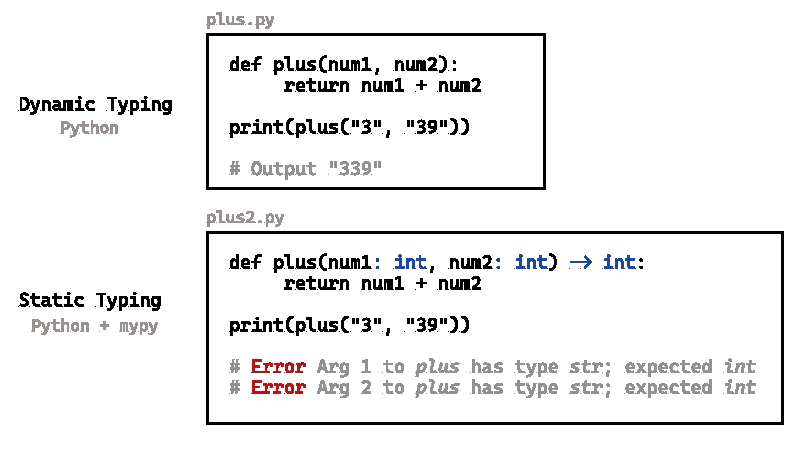
\includegraphics[width=\linewidth]{TypedVsUntyped.pdf}
  \caption{
    \label{fig:typed-vs-untyped}
    Comparison of the same program dynamically typed in Python (Top) and with mypy—a static typing tool for Python (Bottom).  The dynamic-typing rules of the Python interpreter allow it, at run-time, to apply the string concatenating version of the `+' operator -- regardless of the programmer's intention.  By contrast, mypy static-typing checks the type of the values passed to the {\tt plus} function against the intention declared by the programmer through the type annotations on the function parameters (both {\tt int}) and its return type (also {\tt int}).  The type check will fail until the programmer ammends the function call with numeric arguments or otherwise explicitly converts the values from {\tt str} to {\tt int}.
    }
\end{figure}



\section{Functional Programming}

Alongside static typing, \textbf{functional programming} represents another rigorous approach to software development, drawing inspiration from Alonzo Church's lambda calculus in the 1930s \cite{Church1985-bx}. Functional programming treats functions as fundamental building blocks, emphasizing the composition of functions to develop abstractions.

Pure functional programming languages, characterized by immutable values and referential transparency, promote mathematical rigor. Immutable values ensure that once a value is declared, it cannot be altered. Referential transparency guarantees that functions will always produce the same output for identical inputs, providing predictable and testable code.

 A specific subset of functional programming languages, known as `pure' functional programming languages, incorporates additional mathematical rigor through concepts such as immutable values and referential transparency. Immutable values are those that, once declared, cannot be altered. Referential transparency ensures that functions consistently produce the same output for the same input. These properties help mitigate undesirable programming behaviors similar to the way static typing does. For example, the absence of mutable pointers and shared memory in pure functional languages eliminates common concurrency issues like misaligned pointers and race conditions. Consequently, programs developed using these languages are more predictable and can be robustly tested and reasoned about. This significantly reduces the risks that external factors such as network fluctuations or time variations could unpredictably affect program behavior.

Functional programming is often advocated as an excellent choice for introductory programming courses due to its emphasis on mathematical reasoning and strict programming discipline. This discipline includes the clear separation of data from its transformations, fostering a structured approach to problem-solving.


\begin{figure}[hbt]
  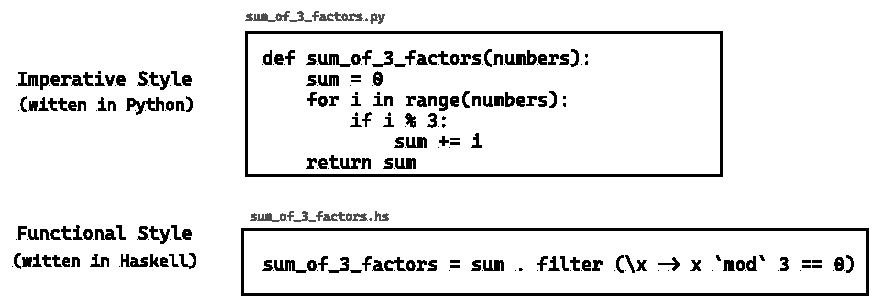
\includegraphics[width=\linewidth]{ImperativeFunctional}
  \caption{
    \label{fig:imperative-vs-functional}
   The same task of summing the factors of 3 in the given numbers, written in imperative style (Top) and functional style (Bottom).
    }
\end{figure}


Functional programming contrasts with other mainstream paradigms like object-oriented programming, which structures programs around objects combining data and behavior, and procedural programming, which focuses on a sequence of procedural steps. Despite the strengths of functional programming, object-oriented and procedural paradigms, exemplified by Java and C, respectively, remain more prevalent in commercial environments. These paradigms benefit from extensive legacy codebases, broad third-party library support, and robust tooling, and familiarity. Lastly, the strictness in functional programming languages may raise the barrier to entry for beginners. For example, in many pure function languages, printing to the terminal window, generally considered a basic technique to observe the execution of the program, requires programmers to understand deep and slightly off-putting concepts like monad and side effects.  


\section{Statically-Typed Functional Languages, The Best Of Both Worlds}
Combining the disciplines described above, \textbf{statically-typed functional languages} employ both static typing and the principles of functional programming. The most common statically-typed functional languages include Haskell,  ML (with the OCaml dialect being the most popular among the family of ML languages), and F\#. 
Of these, Haskell is the only ``pure'' functional language - with all variables being immutable by default.
Descendents of Haskell, like Idris and Agda, include more advanced type-level features like dependent type and session type, allowing programmers to express extremely granular checks of potential software behavior before running the program. These languages often provide the strongest level of programming safety. It is often advertised that programs in these languages will be error-free if the source code passes the compiling stage, indicating that compilers are able to weed out a large number of programming errors. These safety properties allow statically-typed functional languages to be used as proof assistants or formal verification tools. They prove the correctness (or incorrectness) of many systems, from web public key infrastructure \cite{Bhargavan2021-no} to microcontrollers used in space programs \cite{Mokhov2019-zj}. 

Despite these safety benefits, these languages' presence in the mainstream programming world remains underwhelming. This modest popularity is often attributed to high entry barriers, unfamiliarity with the paradigms, and strict type systems that can be daunting for newcomers.

\section{Symptoms of Bad Type Errors}

\ref{sec:symptoms}
 The compiler is the medium through which programmers transform human intention into machine instructions. When encountering errors, compilers often act like Oracles in ancient history, revealing to programmers obscure messages that often lead to huge confusion and a wrong course of action. Many studies have investigated the ineffectiveness of compiler error messages \cite{Barik2017-gy, Becker2019-cs, Becker2016-kc}.  Our exploration is centered around the Haskell programming language and its leading compiler, Glasgow Haskell Compiler (GHC), with the aim of enhancing its handling of type error notifications. It is vital to mention that the challenges discussed here, concerning error messages, are common across compilers for various statically-typed languages. Below, we delve into specific issues often observed in type error messages.


 \subsection{Bias in Type Errors} 
 \label{subsec:bias}
 
A significant issue in type error messages is their inherent bias. Often, type errors can arise from multiple causes, but the error message might only highlight one. This issue is known as left-to-right bias in traditional type-checking algorithms—a notable shortcoming that limits the usability of error messages \cite{McAdam2002-vb, Lee1998-fx, Chen2014-ev}. We will explore this further in Chapter \ref{chap:haskell-type-checking}. For instance, as shown in Figure \ref{fig:type-error-example}, a programmer likely intended to add two numbers using the \texttt{+} operator instead of mistakenly using the concatenation operator \texttt{++}. However, the type error issued by the compiler mistakenly points to the application of the integer literal \texttt{3}, failing to suggest the probable misuse of operators.

 \begin{figure}[hbt]
  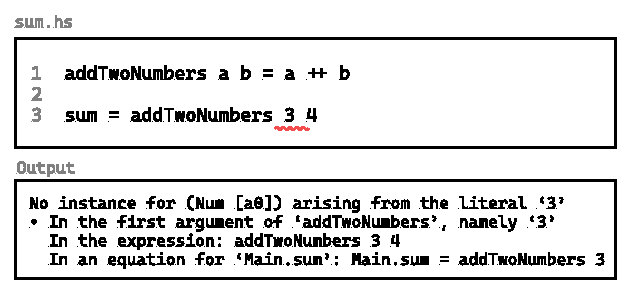
\includegraphics[width=\linewidth]{TypeErrorExample}
  \caption{
    \label{fig:type-error-example}
    Misuse of the concatenation operator \texttt{++} instead of the addition operator \texttt{+} on line 1 is indicated. However, the compiler incorrectly suggests an error due to the use of the integer \texttt{3}.
    }
\end{figure}


\subsection{Type Error Suggests Incomplete Cause}
\label{subsec:imcomplete}

Often, type error messages do not fully present all the locations relevant to the type error. Addressing the error at the highlighted location might not suffice to resolve the underlying problem. Consider the scenario in Figure \ref{fig:type-error-example-2}, where a function intended for list concatenation is erroneously applied to integer values. Here, the error message only reports the first argument, neglecting the second. This partial reporting leads to a situation where correcting the first integer to a list format, \texttt{[3]}, doesn't rectify the error; rather, it only updates to a slightly different error message. 



\begin{figure}[hbt]
  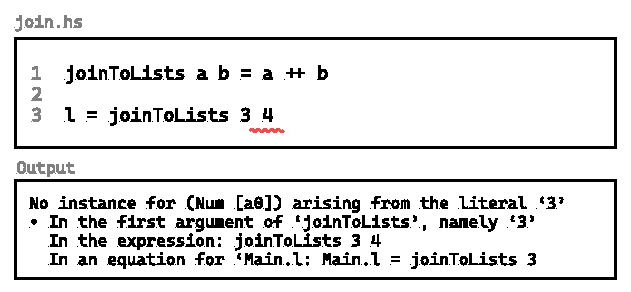
\includegraphics[width=\linewidth]{TypeErrorExample2}
  \caption{
    \label{fig:type-error-example-2}
    A programmer’s attempt to use a concatenation function on integers results in an incomplete error message that only flags the first offending argument. Modifying one argument alone is insufficient to clear the error.
    }
\end{figure}

\subsection{Missing Links In Type Errors}
\label{subsec:missing-link}

One of the most frustrating aspects of type errors is that they do not show the complete pathway of how the compiler decided on the type error. In the example in Fig \ref{fig:type-error-example-3}, the programmer may intend to compare to a char literal \texttt{' '} instead of string literal \texttt{" "}. However, there are multiple clues that contribute to this conclusion: the definition of the function \texttt{trimWhiteSpace}, the application of \texttt{filter isSpace a}, the definition of \texttt{isSpace}, and even the type signature of \texttt{filter} are all needed to understand the logical reasoning. However, none of these are included in the actual error message.


\begin{figure}[hbt]
  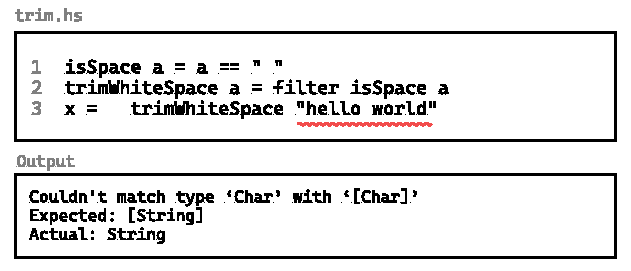
\includegraphics[width=\linewidth]{TypeErrorExample3}
  \caption{
    \label{fig:type-error-example-3}
  This example illustrates how the programmer may intend to compare to a char literal \texttt{' '} instead of a string literal \texttt{" "}; however, the type error ignores all the important clues of how this error is inferred. 
    }
\end{figure}


\subsection{The Use of Obscure Language}

Error messages are frequently plagued by technical jargon and convoluted phrasing, which can be particularly daunting for novices. An example is the error message, \texttt{No instance for (Num a) arising from the literal `3'}, which is an inept way of suggesting a type mismatch involving character and numeric types. In fact, this is often the common behavior across many programming languages and has been shown in many studies \cite{Barik2017-gy, Tirronen2015-nr, Prather2017-dg}. Thus, concerted efforts \cite{Becker2016-kc, Barik2014-ib}  show that rephrasing the error message to be clearer and more structured positively affects programmers' ability to solve these errors.


\section{The Challenges Of Making Good Type Errors}

After introducing some typical symptoms of bad type error messages, we will now explore some fundamental challenges that underpin these symptoms.

\subsection{Types Are Complex}

The advantages of statically typed languages derive from their robust type-checking systems, which, ironically, also introduce significant complexities. Language and tool designers frequently overlook the intrinsic complexity of type systems. In languages that support dependent types, types have the same computing capabilities as runtime programs. This complexity is not limited to dependently typed languages; for instance, type checking in common languages can exhibit Turing-complete characteristics, which might lead to non-terminating processes~\cite{Wells1999-ob}. TypeScript introduces `conditional types', a feature that allows sophisticated computations at the type level \cite{fig:ts-conditional}, posing challenges in explaining errors when these type-level computations fail due to a lack of adequate debugging tools.



\begin{figure}[hbt]
  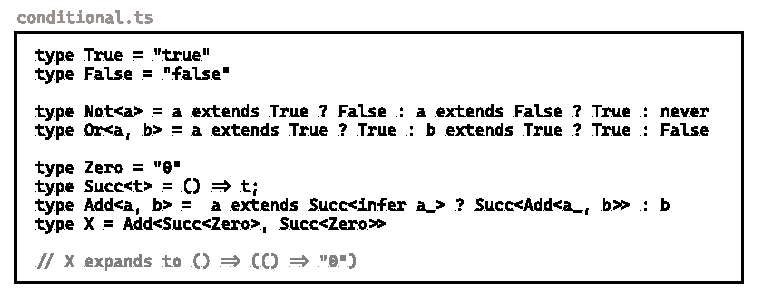
\includegraphics[width=\linewidth]{Conditional}
  \caption{
    \label{fig:ts-conditional}
  TypeScript's feature of conditional types, allows for complex logical conditions at the type level, which can be as complex as the program it annotates.
    }
\end{figure}

\subsection{Clues For Type Checking May Be Implicit}

The task of understanding how types are assigned in a program grows notably more complex when the programming language employs type inference. Type inference \cite{Damas1982-sc} is a technique that allows programmers to forgo the task of writing type annotations. Instead, the type checker automatically deduces the appropriate types for each expression based on the context. Although it succeeded in providing rigorous type checking without the hassle of manually writing type annotations, type inference has been shown to bring many usability issues \cite{Jun2002-xp, Wand1986-lu} for its implicitness.  

Even in programming languages that do not utilize implicit typing, certain typing rules remain opaque to programmers. For instance, rules on permissible values for equality check using the \texttt{==} operator vary across programming languages; some languages disallow comparison of lists, and others are fine with lists but disallow comparison of floating-point numbers. In languages that support a record data type, programmers must navigate additional complexities, such as whether adding or removing a field from a record maintains type correctness \cite{fig:row-polymophism}. This often involves an understanding of nuanced language-specific rules, including concepts like covariance, contravariance, and subsumption.


\begin{figure}[hbt]
  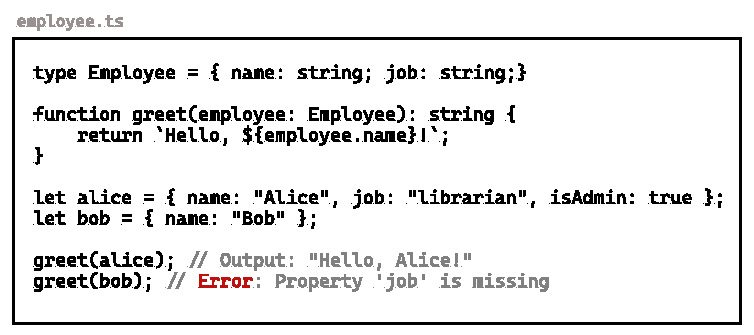
\includegraphics[width=\linewidth]{RowPolymorphism.pdf}
  \caption{
    \label{fig:row-polymophism}
Row polymorphism enhances flexibility in structuring data collections but also introduces complexity in understanding type substitutions and variance.
    }
\end{figure}

These challenges amplify the difficulty in designing intuitive type error messages. The complexity of type systems demands that designers have a profound understanding of both theoretical and practical aspects of language implementation—knowledge often possessed only by the core language developers. Moreover, the implicit nature of modern programming languages requires that type errors be designed on a case-by-case basis, a daunting task given the limited number of contributors who possess the necessary expertise.

\section{The Lack of Type Debugging Tools}

Debugging programming errors has been an unpleasant but crucial part of programming since the inception of computing, tracing back to as early as 1949 \cite{Campbell-Kelly1992-rn}. However, the tools and support for debugging type errors have not evolved significantly and do not match the advancement of those available for runtime errors.

One of the simplest and most dependable debugging techniques is to insert \texttt{print} statements. As computing pioneer Brian W. Kernighan once noted, ``The most effective debugging tool is careful thought, coupled with judiciously placed print statements'' \cite{Kernighan1978-xs}. Furthermore, breakpoint debugging has become a staple in nearly all programming Integrated Development Environments (IDEs), allowing for intermittent code execution and inspection \cite{fig:breakpoint}. Research in error debugging tools continues to be dynamic. For instance, ZStep94 \cite{Lieberman1995-lg} enhances traditional breakpoint debugging by eliminating the need to set breakpoints, thus enabling programmers to view and navigate through the historical values that expressions take throughout execution (Figure \ref{fig:zstep94}). Another innovative tool, WhyLine \cite{Ko2009-uf}, aligns with the principles of a natural programming environment \cite{Myers2004-fy} by allowing programmers to ask ``why'' questions and ``why not'' questions about certain program behavior.

Despite these advancements in runtime debugging tools, the development of type debugging seems to have stagnated. Most programming languages and development environments still handle type errors in ways reminiscent of early languages like FORTRAN and ALGOL. In recent years, some modern programming languages like Elm and Rust have made efforts to improve type error reporting, but these enhancements are often superficial and do not fundamentally change the debugging experience.


\begin{figure}[hbt]
  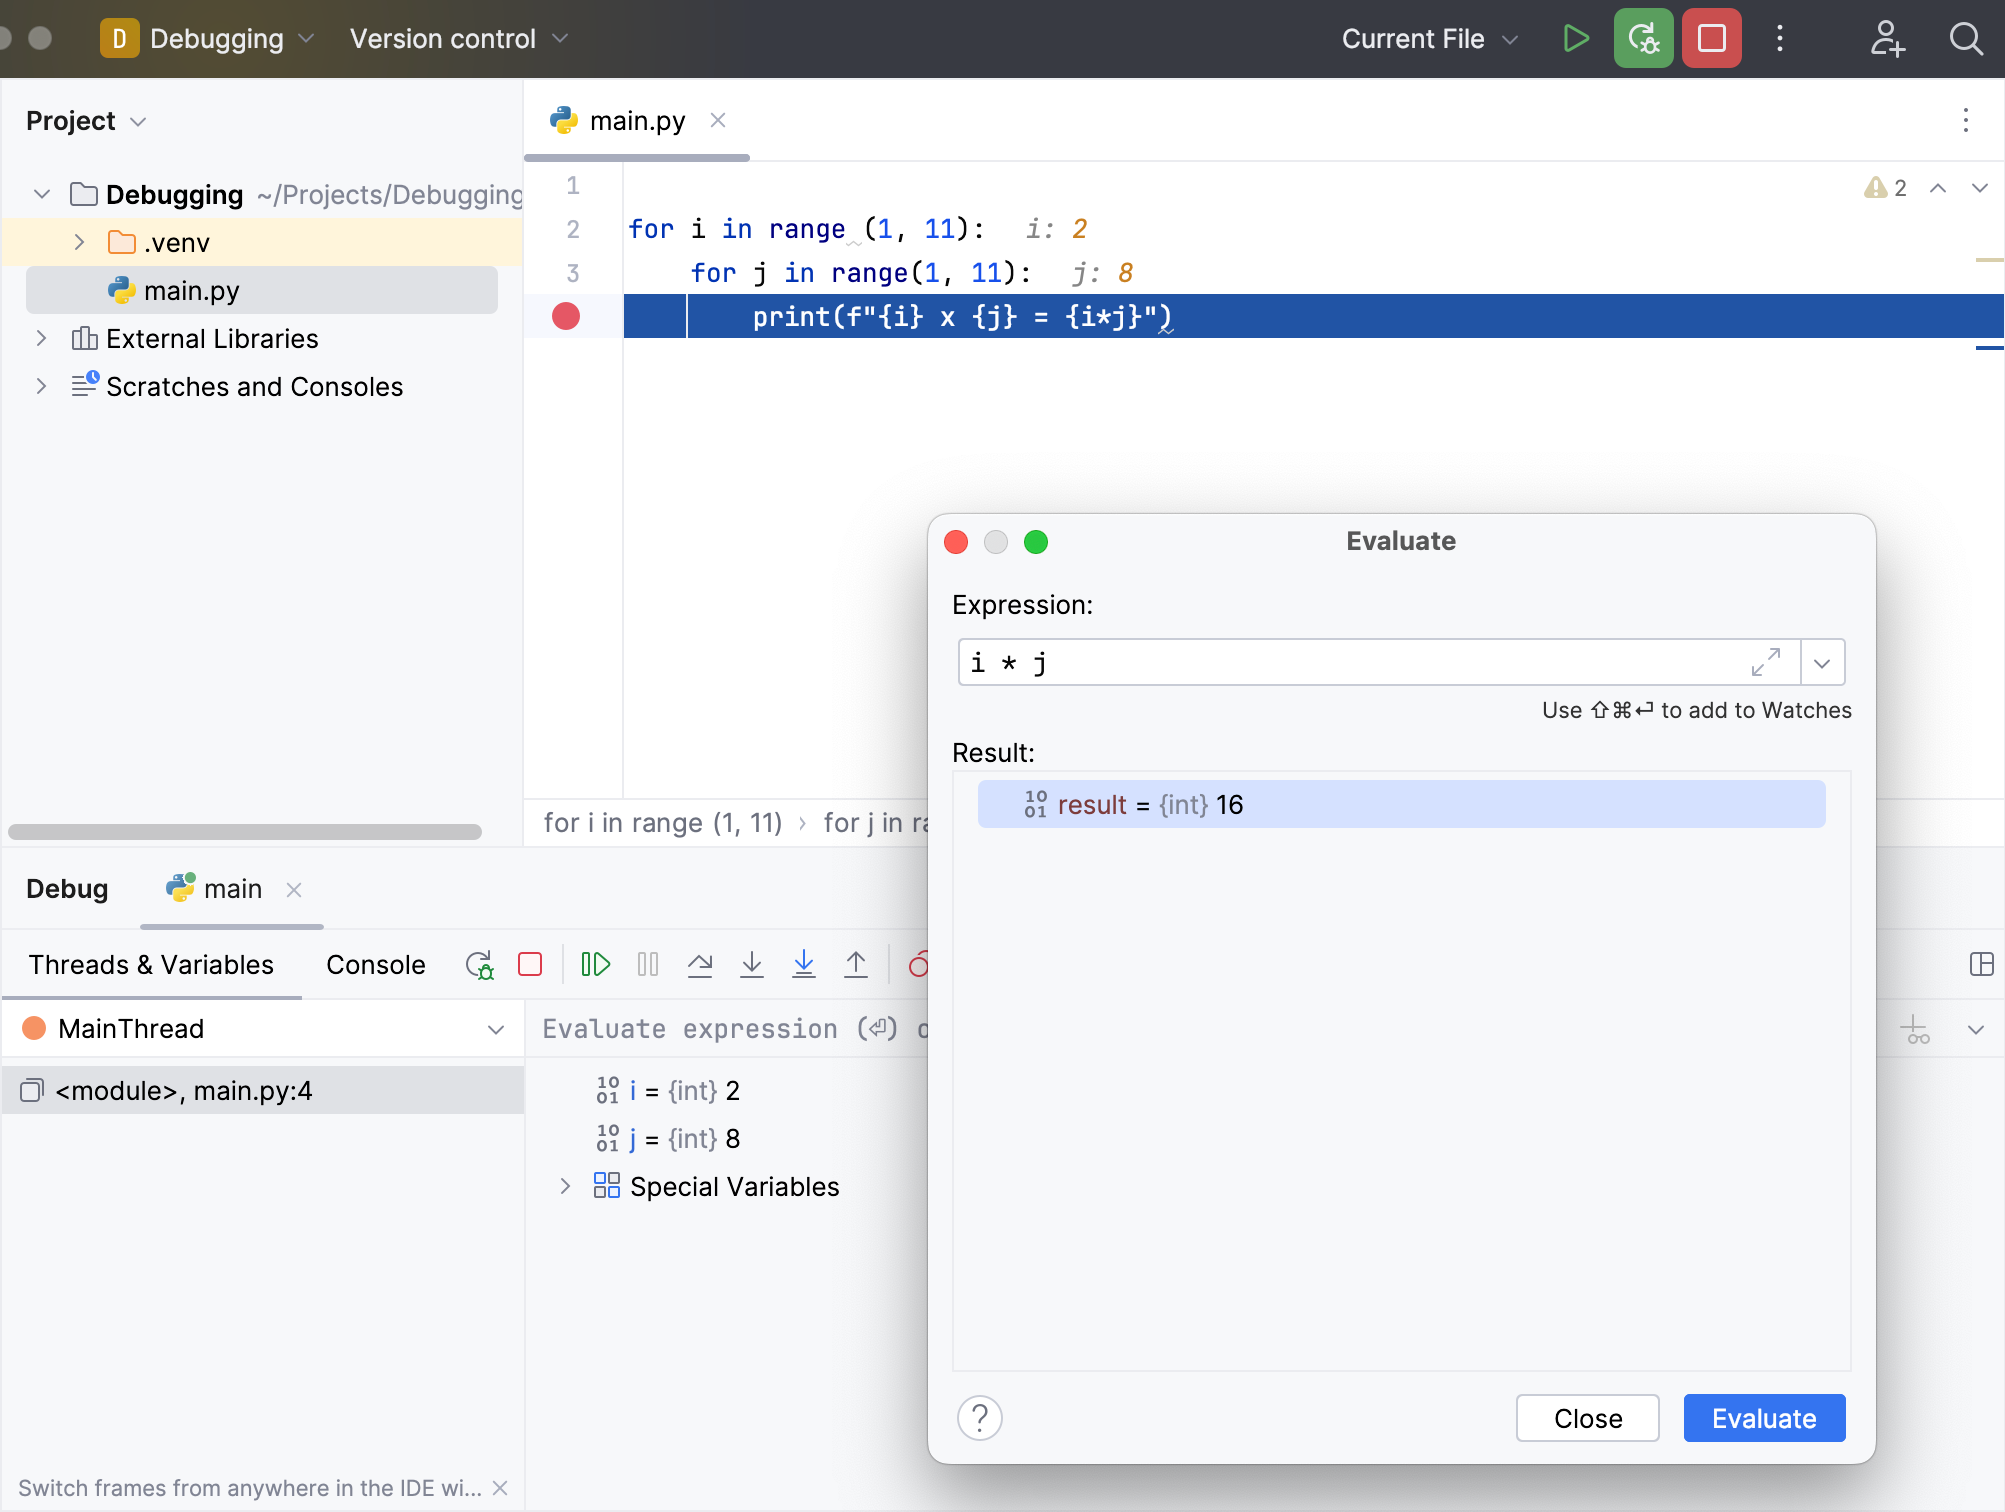
\includegraphics[width=\linewidth]{BreakPoint}
  \caption{
    \label{fig:breakpoint}
    Debugging a Python program using a breakpoint debugger and expression evaluation in PyCharm.
    }
\end{figure}


\begin{figure}[hbt]
  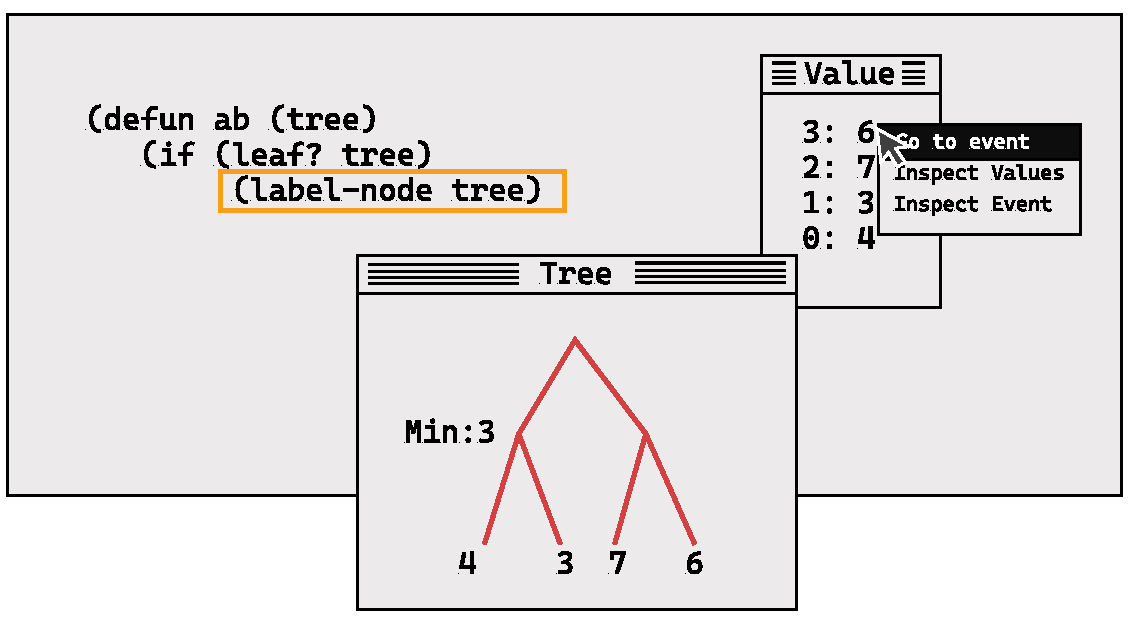
\includegraphics[width=\linewidth]{ZStep94}
  \caption{
    \label{fig:zstep94}
    Debugging a Lisp program by inspecting all the historical values of an expression, navigating through execution history, and reviewing live visualization replay.  All these features are provided in ZStep94.
    }
\end{figure}

My research is driven by the acknowledged difficulties in debugging type errors and the lack of significant advancement in the interfaces and techniques used for presenting and resolving these errors through modern graphical user interfaces and human-computer interaction techniques. This area holds considerable potential for improving both the usability and accessibility of statically typed languages, making them more approachable for developers at all levels of expertise.

\section{Research Aim}

\subsection{Aim 1. Provide Programmers With The Comprehensive Knowledge Needed to Understand and Resolve Type Errors.}
\label{subsec:aim1}

Current representations of type errors in most compiler tools are often insufficient, typically providing only the location of the type check failure, the expected type, and the actual type encountered. This conventional approach, as discussed in the previous sections (\ref{sec:symptoms}), lacks practicality and clarity. This aim addresses the need for a richer, more informative explanation of type errors by evaluating the limitations of existing systems and analyzing how programmers tackle type errors in practice.

\subsubsection{Objective 1.1 To Encompass Multiple Potential Causes Of A Type Error}
An essential aspect of this research is to challenge and expand beyond the bias found in traditional type error reporting (Section \ref{subsec:bias}). It's crucial to inform programmers of multiple potential causes and resolutions. A key goal is to communicate these multiple dimensions effectively. In addition, for each potential cause, programmers need a clear explanation of where the offending code is, which typing rules are violated, and how the type might change after the error is resolved.


\subsubsection{Objective 1.2 To Accurately Report Relevant Locations Contributing to Type Errors.}
Current tools often pinpoint a single location for a type error, a method that has attracted considerable criticism for its inefficiency. Programmers frequently need to scan beyond the initially reported location. This research aims to enhance type error reporting by identifying and detailing all relevant error-contributing locations across the codebase.

\subsubsection{Objective 1.3 To Give Reasons And Support Human Understanding}
Understanding type errors goes beyond pinpointing the location in the code. Internally, type errors can be caused by mismatched types, unmatched type class constraints, or trying to construct infinite types. Externally, type errors can be caused by typos, outdated type annotation, incomplete implementation, etc. Our goal is to not only find these errors but to explain them in a way that logically supports the programmer's understanding and troubleshooting process, covering both internal causes and external causes.



\subsection{Aim 2. Support Programmers To Type Errors Through Interactive Modern Programming Environments.}

This aim focuses on integrating comprehensive type error encoding (Section \ref{subsec:aim1}) within an interactive programming environment to streamline workflows in statically typed languages. It acknowledges that an increase in information does not necessarily correlate with enhanced understanding and aims to present type error details in a way that optimally supports comprehension and resolution.

\subsubsection{Objective 2.1 Visualize The Key Concepts Of Type Errors Effectively}

Traditional text-based error reports can be difficult to navigate and understand. This objective explores innovative methods to present what used to be displayed as plain text (type signatures, locations in source code, call stacks, dependency graphs) in a novel and intuitive way. Examples include in-line highlighting within the code editor and graph-based reasoning steps.  

\subsubsection{Objective 2.2 Use Interactive Tools for Investigating and Resolving Type Errors.}

This research will explore interactive techniques to dissect and explore type errors in a manageable and meaningful way. By breaking down errors into smaller, understandable units, programmers can methodically trace and address the root causes. This includes providing context-sensitive debugging aids that adjust the level of detail presented based on the error type and individual user preferences, ensuring a tailored and effective debugging experience.


\section{Contributions}

\subsection{A categorization of type errors based on the structure of the evidence of a type error}

To address the complexities in explaining type errors comprehensively, we have classified type errors into three complexity categories based on a human perspective. Formal definitions and a detailed discussion of these categories appear in Chapter \ref{chap:haskell-type-checking}. It is crucial to understand that these categories are not mutually exclusive; for example, a multi-witness type error may also be a multi-step type error.


A \textbf{multi-step type error} occurs through a chain of logical inferences steps based on the available evidence of the error. Figure \ref{fig:multi-step-example}) illustrates the chains of inference in the assignment of a (Line 1), the equivalence of a (Line 1 and Line 2), the assignment of b (Line 2), and the equivalence of b (Line 2 and Line 3). Removing any one of the chains will resolve the conflict. Understanding and communicating the interconnections within these chains is crucial to resolving multi-step type errors effectively.

\begin{figure}[hbt]
  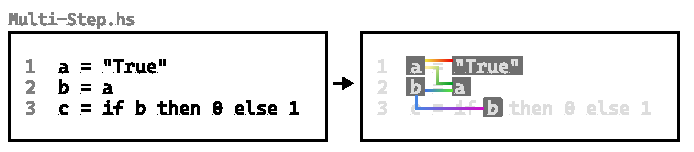
\includegraphics[width=\linewidth]{Multi-Step}
  \caption{
    \label{fig:multi-step-example}
    Illustration of a multi-step type error in Haskell.  The potential issues in the definition of \texttt{a}, \texttt{b}, or the conditional expression of variable \texttt{b}. It can be clearly seen a ``chain'' of reasoning formed in order to explain the type error. }
\end{figure}

A \textbf{multi-witness type error} entails multiple pieces of evidence supporting the same potential type assignments. For instance, as shown in Figure \ref{fig:multi-witness-example}, multiple evidence (lines 3,4,5) support that a has the type \texttt{Int -> String}. On the other hand, a single piece of evidence (line 2) shows that a has the type \texttt{Int -> Char}.  Clarifying and juxtaposing this discrepancy in witnesses is key to supporting understanding this type of error.

\begin{figure}[hbt]
  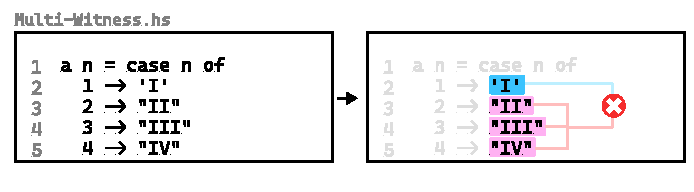
\includegraphics[width=\linewidth]{Multi-Witness}
  \caption{
    \label{fig:multi-witness-example}
    Analysis of a multi-witness type error, where the \texttt{case} expression could be interpreted as type \texttt{Char} or \texttt{String}. This scenario showcases a type disagreement with witnesses (in color pink) against one witness (in color blue). It is not hard to see that the difference in number play an important role here as the char literal \texttt{'I'} on line 2 is more likely be a typo.
    }
\end{figure}

A \textbf{multi-party type error} involves several potential type assignments, each supported by distinct evidence.  Figure \ref{fig:multi-party-example} presents a typical multi-step type error: the expression \texttt{d} can not be assigned a type because 3 pieces of evidence on line 1 suggest 3 potential types for \texttt{d}. In practice, addressing such errors requires decomposing them into multiple type errors of simpler forms.


\begin{figure}[hbt]
  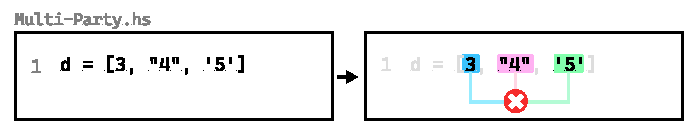
\includegraphics[width=\linewidth]{Multi-Party}
  \caption{
    \label{fig:multi-party-example}
    Analysis of a multi-party type error regarding the list \texttt{d}, which could alternately be typed as \texttt{[Int]}, \texttt{[String]}, or \texttt{[Char]}. The conflict is depicted as a disagreement among three parties (Right). Unlike the previous two examples, this error cannot be fixed by a single location. }
\end{figure}

These classifications have led to the development of three distinct systems—Chameleon, Goanna, and GeckoGraph—each designed to tackle unique challenges within the domain of type error debugging.

\subsection{Explaining Multi-Step Type Errors Through Chain-Of-Thought Visualization}

\subsubsection{Technical Contribution - Chameleon}


We contribute Chameleon, an interactive Haskell debugging tool that not only identifies all relevant error-contributing locations but also illustrates the logical relationships between these locations. Chameleon provides a novel debugging interface to interactively explore the chain of reasoning in a multiple-step type error, allowing programmers to develop a panorama view of the type error interactively. In addition, Chameleon uses an adaptive interface design; programmers can switch between different granularity of information based on their personal preferences. 

\subsubsection{The evaluation on the effect of error slicing and chain of thought visualizations}
We evaluate the efficacy of interactive visual debugging tools in contrast to conventional type error debugging methods. We have conducted studies that assess how programmers resolve type errors using various interfaces ranging from basic type error slicing techniques to Chameleon's step-wise interactive debugging tools. These evaluations aim to measure how enhancements in the debugging process can influence error resolution tasks' efficiency and intuitiveness.

\subsection{Iterate potential causes of multi-witness and multi-party errors}

\subsubsection{Technical Contribution -- Goanna}
Goanna enhances type error debugging in Haskell by not only identifying all relevant error-contributing locations but also dividing the type error into possible causes and their respective resolutions. It ranks these potential causes based on their likelihood, helping programmers systematically approach error resolution.

\subsubsection{An evaluation on accuracy, conciseness, and performance of MCS-based type debugging and our heuristics}
We evaluated Goanna's performance across a diverse set of Haskell programs, analyzing its accuracy and performance in error identification against traditional tools. We evaluate Goanna's conciseness in narrowing down potential causes into a shortlist. 


\subsection{Visualizing Types}

\subsubsection{Technical Contribution -- GeckoGraph}

We contribute GeckoGraph, a graphic notation for Haskell types. GeckoGraph encodes the same information as type signatures but uses colors, shapes, and symbols to make certain structures easy to identify at a glance. GeckoGraph uses visual elements to improve the understanding of complex type concepts, such as type classes and qualified constraints. GeckoGraph offers clarity when reading dense type signatures and comparing multiple types.

\subsubsection{An evaluation on how programmers use graphic type notation}

We contribute a large-scale empirical study exploring the effectiveness of graphical type representations like GeckoGraph in enhancing programmers' abilities to tackle type-related tasks.

% \section{Research Method}

% \subsection{Human-centered programming language studies}

% One important decision that shape a lot of my work is employing human-centered research methods with our novel programming language systems. The adopting of human-centered methods happens at every stage of the projects: prototyping, development and evaluation. Although the using of these methods are not new at all, but they certainly are not the most polular choices in programming language studies.

% The motive of such decision is that it is impossible to understand what are the good qualities of type errors without observing how human use type errors to gain understanding. 


% The downside of study programming language is iterative design is very hard. programming tasks involves complex inputs and outputs, and it is very hard to study an incomplete system without a fully working systems. For instance, if we are to study the effect of type errors, it is most effective to have a system that can recognize type-correct program from ill-typed one. It is hard to evaluate with a mock-up or wizard of oz style fake outputs to study users' interaction.  To address this limitations, we have a few ideas implemented in our research:

% A minimal but practical set of language 
% Design for human from start



\section{Thesis outline}

 This thesis is structured into two main parts. The initial chapters build a comprehensive foundation on type systems and programming languages, setting the stage for my research contribution in subsequent chapters. The latter chapters focus on distinct contributions that tackle various challenges in type error debugging.

\subsection{Chapter 1}
Chapter 1 sets the stage by discussing the fundamental concepts of programming languages and type systems. It explores the trade-off between enhancing program safety and optimizing usability, a central dilemma in programming language research and software engineering practice. The chapter highlights common issues and technical challenges associated with type errors, establishing the motivation for this research. It also outlines the specific aims and contributions of the study, providing a clear roadmap for the thesis.

\subsection{Chapter 2}
This chapter delves into the fundamental concepts underlying type systems and programming languages. It outlines traditional methods employed in Haskell type checking, error slicing, and interactive debugging. Additionally, this chapter discusses tools and techniques used in constraint satisfiability analysis that are integral to later developments in the thesis. The categorization of type errors is revisited and redefined, building on the definitions introduced in this chapter.
    
\subsection{Chapter 3}
Chapter 3 presents Chameleon, a system designed to enhance the debugging of type errors through interactive visualizations. It begins with a discussion on the typical pitfalls of existing error messages and outlines the motivation behind Chameleon. We then detail the system's design, features, and development process, including iterative prototyping. A series of empirical studies were conducted to assess Chameleon's effectiveness compared to traditional compiler tools.
    
\subsection{Chapter 4}
Chapter 4 introduces Goanna, a Haskell type error debugging tool that incorporates novel features such as suggesting fixes for type errors and cross-module debugging capabilities. It starts with highlighting the limitations of conventional compiler error messages and progresses to describe Goanna's capabilities in identifying all causes and ranking potential causes by their likelihood. The implementation tactics and heuristic methods used in Goanna are discussed, followed by an empirical evaluation of the system's accuracy, conciseness, and performance based on real-world Haskell code examples.
    
\subsection{Chapter 5: GeckoGraph — Visualizing Haskell Types}
The final chapter synthesizes the thesis's contributions and situates them within the broader research context. It discusses potential avenues for future tool development and research opportunities, forecasting the future landscape of research in type error improvement. The chapter concludes with reflections on the expansive and still largely unexplored territories in programming languages, encouraging ongoing investigation and innovation.

    
\subsection{Chapter 6: Conclusion}
The final chapter synthesizes the thesis's contributions and situates them within the broader research context. It discusses potential avenues for future tool development and research opportunities, forecasting the future landscape of programming language research. The chapter concludes with reflections on the expansive and still largely unexplored territories in programming languages, encouraging ongoing investigation and innovation.


% Chapter 2

\chapter{Background}
\label{chap:background} 

Programming in strongly typed languages has many advantages. It helps programmers identify logical errors before running the code, reduce maintenance difficulty, and improve the editor capability find documents and auto-complete code while typing. However, the difficulties in understanding and resolving type errors often ward people off  from practicing strongly typing.  In this Chapter, we discuss the relevant research in improving the experience of debugging type errors. We first investigate the theoretical approaches to enrich/correct the information presented type errors. We then  investigate the various designs of tools, interfaces, and visualizations to support understanding type errors.

\graphicspath{{Figures/Background}}


\section{Functional Programming}

Functional programming is a programming paradigm that treats computation as the evaluation of mathematical functions and avoids changing state and mutable data. The roots of functional programming are deeply embedded in mathematics, stemming from the lambda calculus - a mathematical system built around function abstraction and application - developed by Alonzo Church in the 1930s.


The early functional programming languages include Common Lisp in the 1950s, Scheme invented in the 1970s, and ML in the 1970s. In the 80s  the language Miranda was developed, introducing the world to more flexible functional concepts, such as lazy evaluation. However, some of these ideas were commercialised, which spurred the creation of Haskell – a purely functional language produced by the open-source community, later becoming a seminal achievement and most influential functional language in academia and the programming industry.


In the 21st century, although new functional programming languages are continue to be created, such as Clojure, F*, and Idris, what’s more often interesting to see is functional programming ideas and benefits into other paradigms. Scala is a programming language that combines the expressiveness of functional composition and ergonomics of object oriented programming. JavaScript, a traditional multi-paradigm language, started to adopt programming features such as lexical scoping, tail recursion optimization.


In 1978 John Backus delivered his Turing Award lecture, “Can programming be liberated from the von Neumann style?”, bringing functional programming into the recognition in the larger programming world. Different from other paradigms in the programming realm, functional programming brought a few innovations that changed the thinking in the academic and programming community, and has been sought after by other paradigms for decades to come.


\textbf{Declarative}: being close to mathematical functions, functional programs are the composition of forms that map value from one domain to another. Instead of explaining how to achieve a specific task step-by-step (like in imperative languages), functional programming encourages developers to describe what they want to achieve and the language abstracts the how.


\textbf{Immutability}: Unlike object-oriented programming, where data structures (such as objects) could be changed, or mutated, data in functional programming is immutable, meaning it cannot be changed after creation. This trait reduces the chances of bugs because you know that your data isn't changing unexpectedly.


\textbf{Pureness}: pure functions are functions that observe referential transparency, in other words when given the same input will always reach the same output. The pureness of functional programming seems to be a big restriction and handicap on what a function can do, for instance, that pure functions cannot access external systems or produce true random numbers. However, pure functions are as potent as they are limiting, it creates a strong separation between data and programs and powerful transformation can be developed on the premise that no side effects are present in the programs.


\textbf{High order functions}: The idea of using functions as normal values where they can be assigned to names, returned by other functions, or passed as arguments is a fundamental ingredient of functional thinking. This aspect allows programmers to create more abstract functions and reusable logic. Currying is a special case of high order function, where a function with multiple arguments is transformed into a sequence of functions, each with a single argument. Currying is beneficial for creating simpler and cleaner functions and aids in code reusability.

\section{Statically Typed Languages and The Typing Debate}


Static typing has been practised since the very start of programming languages. Fortran, known as the first compiled programming language, has explicit types for integers and floating point numbers, and uses static typing to reject mal-formed programs. Later programming languages Pascal, C were all designed to use static typing. In these languages, user defined types, such as functions and structs, have become available, making the type checking more flexible and reliable.

 
Functional languages, especially Haskell, took the static types further with ideas coming from academic languages, such as typed lambda calculus and system F, that are shown to be sound and complete. Many type-level features in Haskell were later exported to languages of other paradigms.  Polymorphic types were introduced to allow functions types to be defined more fluidly so that they can work with any data types. Type inference (also known as implicit types) was introduced to allow static type checking even without any explicit type annotations. These features can now be found in most mainstream programming languages. (Give an examples of )


Compared to static typing, the alternative typing discipline – dynamic typing – provides many appealing benefits, and has strong influence in the computing world. In dynamically typed languages, a variable can hold different types of values because the type is checked during runtime. This provides more flexibility than static typing since a single variable can be used to hold different types of values through mutation or reassignment. However, it also means that errors such as trying to subtract a string from a number can be detected only when the code is run, leading to potential runtime errors.


The lisp programming languages, such as common lisp and scheme, were designed to benefit from the flexibility of dynamic typing. In Lisp languages, functions often take dynamic input that can be various forms (atom, lists, s-expressions), and different code is executed based on inspecting the input value at runtime. In modern day computing,  languages like JavasScript, Python are all dynamic languages, which is believed to contribute to their immense popularity thanks to the lower barrier of entry.

\subsection{The arguments for static typing}
\textbf{Program safety}: Static typing can catch errors and bugs during compile time, before the software even runs. This can be particularly beneficial when working on large code bases or complex systems.

\textbf{Ease of Maintenance}: Static typing allows common software engineering tasks, such as refactoring code more reliable. In general, a software project will not successfully compile unless all the  locations affected by the initial changes are addressed and resolved.

\textbf{Additional Tooling Support}: The type information in static languages can help programmers understand code better and faster. This is often shown as richer information in documentation, or more detailed pop-over type hints with modern programming IDEs.  

\subsection{The arguments for Dynamic typing}

\textbf{Ease of Use and Flexibility}: Dynamically typed languages usually have a simpler syntax, and the flexibility of being able to change the type of a variable on the fly.

\textbf{Rapid Prototyping}: Dynamic typing can be faster in terms of development, facilitating quick prototyping and scripting.

\textbf{Metaprogramming}: Dynamically typed languages are robust in metaprogramming because they can inspect, generate, and modify code more flexibly during runtime.


\section{The Mission To Improving Type Errors}

Type errors can be notoriously difficult to understand and use, particularly for newcomers to programming or when using a language that is more strict about types. Type errors are often believed to be a major contributor to static typing's popularity. Type errors can happen in dynamic languages as well, however, they are not as difficult as their counterparts in static languages.

Comparing to other programming errors (parsing errors, runtime errors), type errors have some distinct characteristics that render them particularly challenging. 

\textbf{Lack of runtime values}
Types are computed at compile time, and just like the evualting programming sematics, the type checking computations can be complex. In fact, many programming languages type checking are shown to be non-terminating and turing compelte.  Unlike runtime evaluation, type checking cannot be inspected using conventional tools. Inserting print statement inside type annotation is not possible. 

\textbf{Clues for Type Checking are Implicit}
Understanding type assigments of the program become more challenging when the programming language uses implicit typing. Implicit typing, also called type inference, is a technique that allow programmers to omit the ritual of writing type annotations all together and the type checker will infer the most general types (principal types) for each expression. Even for languages that don't employ implicit typing, some typing rules are hidden from programmers.
For example the \texttt{if} expression in many programming languages. The semantics is very clear, but the typing rules are hidden.


\textbf{Lack of tool support}
Lastly, few tools are dedicated on supporting type erros. Runtime programming errors have been studied thouroughly as a research subject and numerous industry tools are focus on understanding and solve runtime errors(GDB, breakpoints, time travel debugger..)  However, in comparason, tool support type error  remain the same depth and capability as they were many decades ago. Most the programming environments render type errors verbatem to the terminal.   


To start, the languages used in type errors are often unhelpful to programmers. On one side, type errors often involve terminology and concepts that can be difficult to understand, particularly for less experienced programmers. The concepts might include objects, instances, classes, functions, variables, or aspects of data types that haven't been encountered before or fully understood. This is exemplified to extremes in Haskell, where programmers are often perplexed by errors like “No instance for (Num Char) arising from the literal '1'”. One another side,  the error messages returned for type errors are either vague or misleading. They might indicate the line of code where the error was detected but the actual mistake might be somewhere else.


Another factor of the difficulty of type errors is the lack of supporting information. Programmers can get stuck in a type error for hours and concede that dynamic languages are easier. When type errors are at runtime, programmers can at least run the program and insert printing statements to observe the dataflow of the program. None of these debugging techniques work on type errors as they are reported without actually running the program.  This is  comparable to debugging parse errors, which also happen at compile time. But generally parse errors are often local, meaning that a parse error has a sensible range of locations,  indentation errors can be searched in the parent indentation block, unmatched brackets can be searched in the outermost brackets. On the other hand, type errors are more global, a type conflict can happen between two different files, or code from different sources. This added to the difficulties of solving type errors.
 

Type errors are made harder with more advanced type system features have been introduced. As a result the usability of type systems decreases as the expressiveness of the type system increases. For example polymorphic types allow types to be defined to restrict the relations between types instead of the types themselves. For example the (==) :: a -> a -> Bool function can be defined to compare two values of the same type, without specifying which type it must be. However, this will add confusion when too many polymorphic variables are participating in the type error and compilers sometimes rename them to further mystify the case.


Throughout history, many have dedicated their research to improving type errors, making them easier to understand and better at helping to find the root causes. We categorise them into three major themes: Enhanced compiler error message, reporting multiple nodes, and interactive debugging.

\subsection{Enhanced Compiler Error Messages}

A well-studied approach to producing better error explanations is through ECEM (Enhanced compiler error message).  As put in~\cite{Barik2017-gy}, ``Error messages appear to take the form of natural language, yet are as difficult to read as source code."   Through a series of mixed-method studies, Prather showed~\cite{Prather2017-dg} that ECEM has a positive result in understanding compiler errors. Decaf~\cite{Becker2016-kc} is a tool that can rephrase Java compiler error messages into an enhanced version. In a study of over 200 CS1 students, Decaf was shown to reduce overall errors in their coding practices. Berik proposed a framework~\cite{Barik2018-xs} for constructing compiler error messages based on argumentation theory, and showed that error messages following a simple argumentation layout or an extended argumentation layout are more human-friendly.  These works show the significance of improving the language in the compiler error messages. 


\subsection{Reporting Multiple Nodes}

\begin{figure}[hbt]
    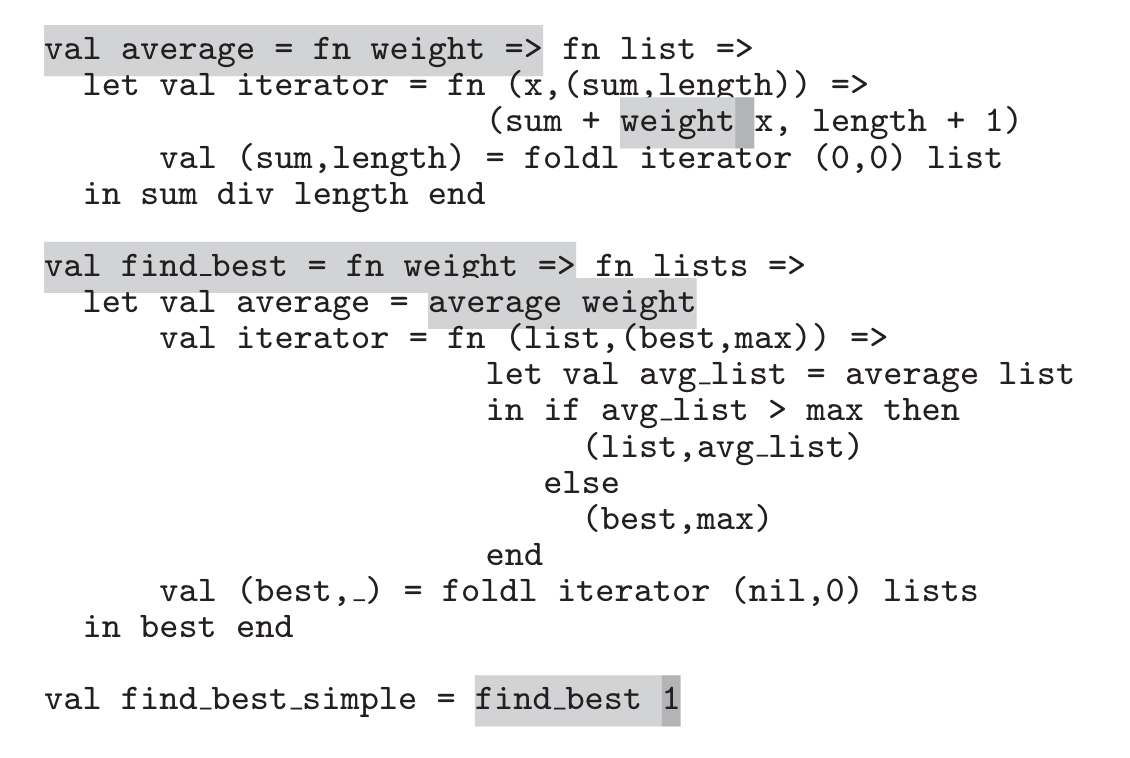
\includegraphics[width=0.6\linewidth]{HaackTypeErrorSlicing}
    \caption{An example of Type Error Slicing by Haack and Wells
    }
\end{figure}

Many have studied the approach of finding all locations that contribute to a type error~\cite{Stuckey2003-pz, Haack2004-fr, Pavlinovic2015-ke, Schilling2012-iq}. Type error slicing~\cite{Haack2004-fr} is a technique that finds locations that are complete and minimal for the type error. Internally labeled constraints and Minimal Unsatisfiable Subset (MUS) generation are used to generate these slices. The language supported in Haack's work was a subset of Standard ML. The original Chameleon~\cite{Stuckey2003-pz} used  Constraint handling rules (CHR) to support the computing of type error slices in Haskell. Chameleon also supported advanced type-level features (type classes and functionally dependent types). The project also introduced the ability to query type information through a command line interface. Although Chameleon was firmly grounded in results from type theory, its designs were never evaluated with user studies. While finding all error locations is useful in comprehending type errors, it is only 1 of the 7 properties listed in the proposed manifesto of good type error reporting~\cite{Yang2000-wn}.

\subsection{Interactive Debugging}

\begin{figure}[hbt]
    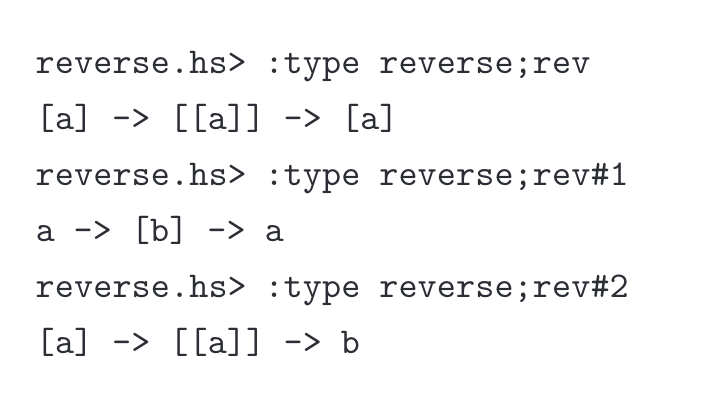
\includegraphics[width=0.6\linewidth]{ChameleonInteractive}
    \caption{An example of Type Error Slicing by Haack and Wells
    }
\end{figure}
Interactive debugging is a method in which programmers can selectively view the debugging information, test and retract their assumptions, and  make changes and observe their effects. Interactive debuggings have been practised for a long time for debugging runtime errors. Programmers often use techniques such as pause/break (also known as a breakpoint) a running program, inspect the current state, and change values if needed. It's highly beneficial because it allows the programmer to interact with the program at runtime, which can provide valuable insights into the state of the program and help identify errors. However, for type errors, programmers are stuck with static error messages in text form. However some early ideas of interactive debugging were proposed in research. Chameleon is an Haskell interactive type debugger that works in command line interface. When encountering a type error, Chameleon is able to analyse and deduce alternative ways a type error can be fixed, and programers can select an alternative they desire by typing in command.


\section{Verify Generated Source Code -- a case for the future}

One trend we have seen in recent years is that generative AI models are widely used to generate code. Once trained, these models can generate code snippets or complete applications based on user input. This might take the form of a natural language prompt, a framework or blueprint layout of the needed application, or even a sequence of tasks or features the code is intended to address. Many models trained in large corpus of software projects show competence in producing source code according to human prompts. However, it seems inevitable that source code generated by a large language model may contain errors, undesired behaviours, or even critical security vulnerabilities. Another big concern is that it is hard to get a grip of the accuracy of AI generated code with popular metrics. In this, human evaluation is still significantly better than automated metrics.


 We believe that statically typed functional languages are the ideal candidates for code generations of these tools. The functional requirements force the pure functions and effect to be clearly separated, where undesired behaviours, such as making database connections, or sending network packets to an external party, are harder to sneak in. In addition, the static typing forces that the generated code must be conformative to the specification. And thus, we strongly believe that now more than ever, we need intuitive type error messages, and streamlined type error debugging processes, to accommodate traditional human written programs, and to tame the AI generated code.


 \section{Conclusion}
 In this chapter, we followed the footsteps of the historical development of functional programming languages and statically typed languages, and their current status in academia and the programming industry. We showed through multiple studies where there is a lack of attention in the design of type errors. We explored multiple research projects that were dedicated to improving the type errors and the way programmers debugging them. We also took a peek at the potential future of programming, and how our effort in improving type errors may help brighten such a future.
% Chapter Template

\chapter{Haskell Type Checking} % Main chapter title

\label{chap:haskell-type-checking}

\graphicspath{{Figures/HaskellTypeChecking}}
In this chapter, we delve into the overview of the technique of type-checking Haskell programs. Haskell uses static types, meaning that type-checking algorithms are run at the time the user compiles the code. More specifically, this happens after the parsing is complete (as the complete syntax tree is necessary for type checking), and before any low level code is generated. In a most simplistic sense, type checking returns a binary result: the program is type correct, or it is ill-typed.

\section{Why Haskell}

The main contributions of my thesis are all in the theme of developing systems to improve the programming in Haskell. Despite all the works being developed to be easily extended to another language, there are important reasons why we implemented these tools for Haskell.

\subsection{Haskell In Education}

Being one of the goals of the  Haskell language, teaching programming in undergraduate computer science courses is an important application of Haskell.  Many text-books meant for first-year computer science courses and introduction to functional programming use Haskell as the learning tool \cite{Bird1998-kv, Davie1992-xv}. Although enthusiasts often argue that Haskell is an ideal platform to teach pure function thinking, real-world university adoption appears to be underwhelming. In fact, helping students tackle programming errors in Haskell seems to be a common challenge in teaching Haskell \cite{Jun2000-yu, Tirronen2015-nr}. Some suggest teaching Haskell with a reduced feature set to prevent the frustration of complex type errors \cite{Heeren2003-mz}. Our research is hugely motivated by the drive to realize Haskell's educational value as well as the challenges of teaching Haskell in real life.

\subsection{Haskell In Mathematics and Formal Logic}

Another important application for Haskell is its application in discrete mathematics and formal logic. Because of its strong type system and enforcement of purely functional computation, Haskell has been standing in the middle of general-purpose programming language and proof assistance. Tools like QuickCheck \cite{Claessen2000-rl} have eased the barrier to writing verifiable programs and have since been borrowed to other languages as well. Some proposed using Haskell in hardware verification \cite{Bjesse1998-lh}. However, a common challenge of using these formal systems is its expandability. As larger proof has been constructed by numerous levels of abstraction, our confidence in the system and ability to explain is lowered. Our research proposes such an interactive explanation system that allows users to check the development of a proof or refutation step by step, each time with a small amount of mental burden. 


\subsection{Haskell's Relatively Small Language Specification}

Although the full language semantics of Haskell were never able to be formally defined \cite{Hudak2007-kn}, it does not stop the language from being studied for programming language innovations, nor does it stop researchers from making meaningful contributions using this language as a platform. Many efforts have been made to formalize subsets of Haskell language \cite{FaxEn2002-nd}. Our research in Haskell benefits from the relatively small language specification, which allows us to quickly implement new ideas and seek feedback.  We also benefit from the welcoming and vibrant Haskell community to help steer our efforts towards better usability. 




\section{Hindley-Milner Type Inference and Algorithm W}

Type inference, also known as implicit typing, is a technique to reduce the number of occurrences of manually ascribing types. Almost all languages today employ a certain level of type inference. For instance, in Java before 10, a common pattern is a user has to declare a variable with a type, often by writing down the class name, and then to initialize the variable, again using the same class name \ref{fig:example-java}. This clearly leads to duplicated knowledge and verbose programs. This has been addressed in later versions (Java 10 and later) by using the \texttt{var} keyword \cite{noauthor_undated-an} to declare variables, and the types of the variables can be guessed at compile-time based on the right-hand-side of the assignments.  

\begin{figure}[hbt]
  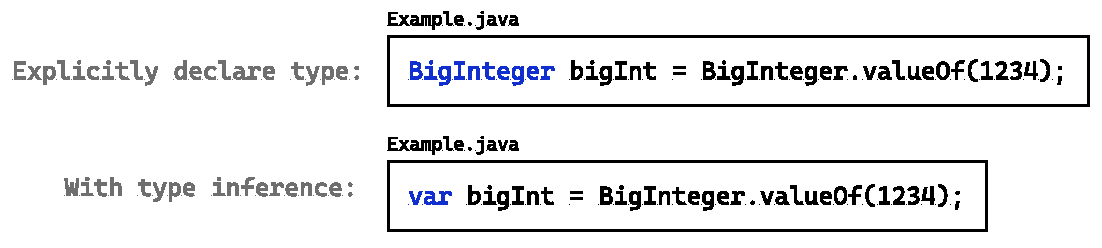
\includegraphics[width=\linewidth]{ExampleJava}
  \caption{
    \label{fig:example-java}
      An example of a typical Java program before and after introducing the \texttt{var} keyword. Before (Top), programmers have to annotate the type, which is identical to the value initializer. After Java 10, this is solved by using the local type inference with the \texttt{var} keyword (Bottom).
    }
\end{figure}

In language like Haskell and ML, not only is type inference applied, but its power to detect type error is hugely amplified by the use of the Hindley-Milner type inference. Unlike the example in \ref{fig:example-java} where type inference happens within the assignment statement, meaning that the compiler will complain if it cannot gather enough information about the type when analyzing this line, with HM-based type inference, the compiler will delay making any assertions, and continue type-checking the rest of the program. 

The Hindley-Milner Type System \cite{Damas1982-zw} is a foundational part of type inference in many functional programming languages, including ML, Haskell, and Elm. The Hindley-Milner Type System, named after its inventors Roger Hindley and Robin Milner, is a type system that can automatically infer the types of expressions in a language with no annotations required. The system provides polymorphic typing, meaning that a variable can be assigned multiple different types automatically based on its usage context, making it easier to write flexible, reusable code without compromising type safety. In many languages that use this system, it is proven that every expression will be assigned a most general type (principal type) based on its usage. 



\begin{figure}[hbt]
    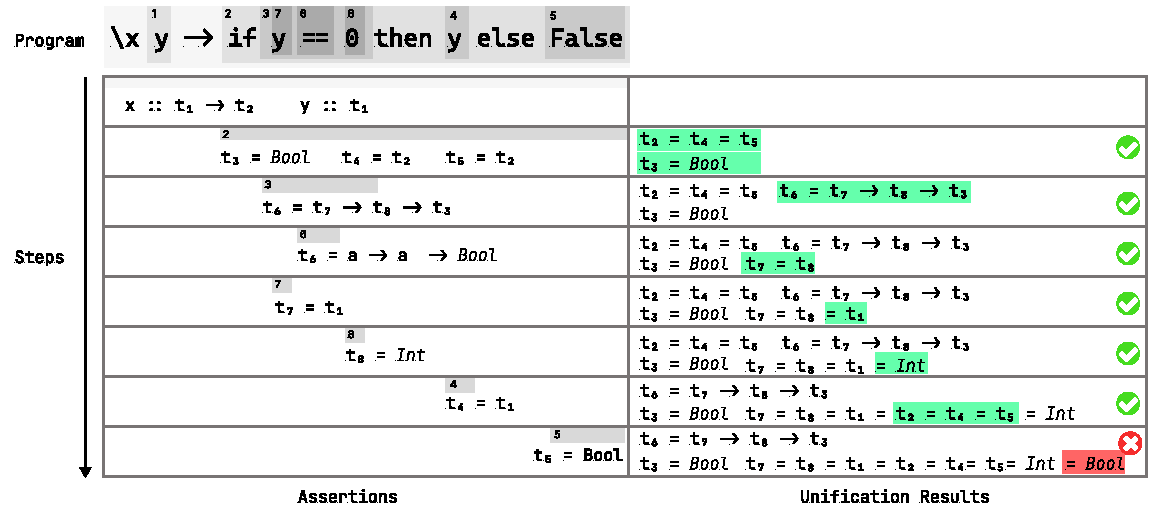
\includegraphics[width=\linewidth]{Hindley-Milner}
    \caption{
      \label{fig:hindley-milner}
        An illustration of Hindley Milner Type Checking}
\end{figure}


\textbf{Algorithm W} The original version of the Hindley-Milner type system uses an algorithm -- W -- to identify the most general types for every expression. Algorithm W scans the whole program and produces the most generous types for each expression. The algorithm works by first assuming that each expression has a unique type variable associated with it,  it recursively inspects into the substructure of the program, and collecting constraints and apply unification \ref{fig:hindley-milner}. Depend on the type of syntax node, during a step new variables may be created, variables may unify with other variables or concrete types. If at any time the unification step fails, the type-checking stops, and the location from which the last constraint is generated will be reported as a type error.


Despite the seismic influence in type theory, and the conciseness of programming style it helps achieved,  Hindley-Milner type system introduced some setbacks in terms of usability. More specifically, its error message when unable to complete the process of type inference leads to a lot of confusions to the users. 

Because of the way unification is carried out, only one constraint (the last one added) is reported in the type error, and the other end of the conflict is unable to be retrieved. Unlike in the Java example, where programmers only need to scan the source code for one line, with the Hindley-Milner-based type system, the potential root cause may lie anywhere in the source code.

\textbf{Algorithm M} 
Others proposed a similar algorithm M \cite{Lee1998-fx}, which, instead of carrying out type inference bottom-up, carries the outer constraints into the inner structure, achieving a top-down type inference and better error messages in some cases. 

\begin{figure}[hbt]
  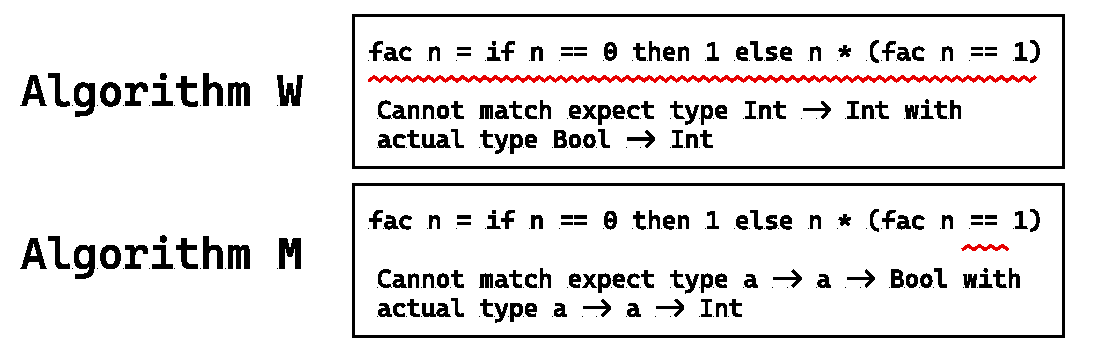
\includegraphics[width=0.8\linewidth]{AlgorithmWM1.pdf}
  \caption{
    \label{fig:algorithm-m-1}
      An example where Algorithm M out-guessed Algorithm W, reporting a more plausible error location.}
\end{figure}


\begin{figure}[hbt]
  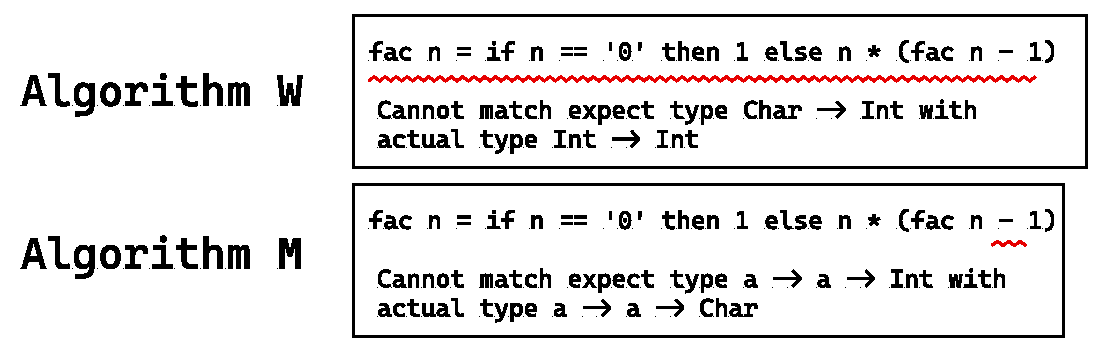
\includegraphics[width=0.8\linewidth]{AlgorithmWM2}
  \caption{
    \label{fig:algorithm-m-2}
    An example where Algorithm M may miss the correct location. It is more plausible here that \texttt{'0'} is a typo.}
\end{figure}


As a result, algorithm M is able to identify certain errors more accurately than algorithm W \ref{fig:algorithm-m-1}. However, it is equally misleading in some other cases \ref{fig:algorithm-m-2}. An important lesson that can be learned from this different approach to type inference is that there is no method that will ensure the result will match the programmers' true intention with the code. At the core, algorithm M and algorithm W suffer from the same issue: the unification is done one step at a time, and the earlier constraints are lost once they are successfully unified. Rather than ambitiously pinpoint the place where the root cause lies, a more realistic goal might be to succinctly represent type error without making assumptions.



\section{Type Error Slicing}

Type error slicing \cite{Tip2001-qn, Haack2004-fr} is a technique that aims to represent type error by including more useful information for the programmers. Compared to the Hindley-Milner approach, it relies on delaying the unification until all constraints are generated. Two important ideas have been employed in type error slicing: 


\begin{enumerate}
  \item {
    Labeled constraints. Assign constraints to locations in programs, and these locations are later on retrieved and identified as part of the error diagnosis. 
  }
  \item {
    Minimal unsatisfiability analysis. Finding the minimal unsatisfiable locations that contributed to a type error  as a standard process of type error diagnosis. In practice minimal unsatisfiable locations avoid being too general as in algorithm W, and avoids being too biased as in both algorithm W and algorithm M. 
  }
\end{enumerate}


\begin{figure}[hbt]
  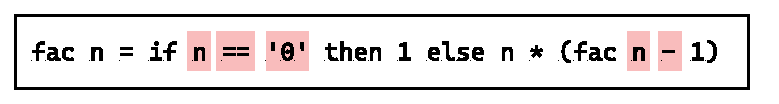
\includegraphics[width=0.5\linewidth]{TypeErrorSlicing.pdf}
  \caption{
    \label{fig:type-error-slicing}
      An example of type error slicing}
\end{figure}

Compared to traditional tools, type error slicing shows complete error locations \ref{fig:type-error-slicing}, and programmers are able to reason about the type error because both sides of the typing conflict are included. 

Over the years, type error slicing has become the go-to approach for optimizing type errors. The method of producing minimal, unsatisfiable locations has been improved and generalized by many. The process generally involves removing constraints one at a time and checking the feasibility of the system changes. Different underlying constraint languages have been studied to encode more advanced type system features. This includes using SMT \cite{Pavlinovic2015-ke}, Constraint Handling Rules \cite{Stuckey2003-pz}, and so on. 



\section{Interactive Type Debugging}

In conventional program slicing approaches, a Minimal Unsatisfiable Subset (MUS) is typically used to represent a single type error, thereby providing locations for the type error report. However, we have identified two significant limitations inherent in MUS-based localization and diagnosis:

\begin{figure}[hbt]
  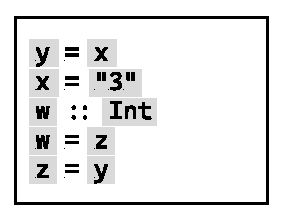
\includegraphics[width=0.5\linewidth]{SlicingCounterExample}
  \caption{
    \label{fig:slicing-counter-example}
      An example where type error slicing essentially highlights every location in the program.}
\end{figure}

MUS-based error slicing can effectively eliminate program locations that are not contributing to a type error. However, research indicates that program slicing can effectively reduce only around 30\% of the code size that is required to understand a type error \cite{binkley_empirical_2007}. Further reduction is challenging with the knowledge of MUS alone due to the MUS's minimality. For instance, in the code shown in \ref{fig:slicing-counter-example}, type error slicing essentially highlights every location in the program. Clearly, there is more important information that needs to be encoded in the type error.

Chameleon \cite{Stuckey2003-pz} is a project that was created as a command-line tool in the early 2000s to improve type error reporting 
for the Haskell programming language. Similar to other type-error slicing approaches, Chameleon used a more general constraint language -- CHR -- which in turn allows more flexible constraint relations to be defined in the constraint language. This is signified by the successful support of advanced type-level features such as type class and functional dependencies. More importantly, Chameleon employed the notion of interactive type debugging. In the example, Chameleon not only highlighted all the relevant locations but it also reflects the fact that two sets of potential types (most general unifiers) can be found in the ill-typed program, and they can be traced back to two sets of locations in the source code. Programmers can proceed to query the type information of either potential resolution as if the type error has been resolved.


\begin{figure}[hbt]
  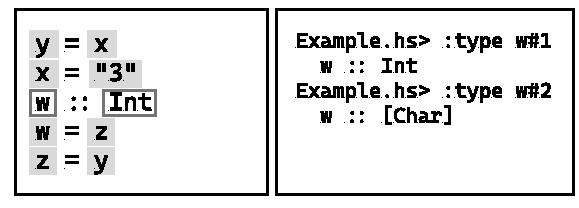
\includegraphics[width=0.8\linewidth]{ChameleonInteractive}
  \caption{
    \label{fig:chameleon-interactive}
      An example where type error slicing essentially highlights every location in the program.}
\end{figure}

\section{The Analysis Of An Unsatisfiable System}

One advantage using a holistic consstraint solving appraoch is that many tools are available from the study of constraint satisfiability. In this, the most useful tool we use are the Minimal Unsatisfiable Subset (MUS), Minimal Correction Subset (MCS) and Maximal Satisfiable Subset (MSS).  

\subsection{Minimal Unsatisfiable Subset}

MUS is the most commonly used appraoch. Most program slicing based tools \cite{Haack2004-fr, Pavlinovic2015-ke, Stuckey2003-pz} use MUS one way or another. Intuitive, MUS is the smallest subset of constraints syetm that still remains infeasible. Infeasibility simpliy means there are no ways to assign value to the logical variables. For an ill-typed program, this means finding a minimal set of locations that contain a type error. 

Formally,  a minimal unsatisfiable subset (MUS) $M$ of a constraint system $C$ is a subset $M \subseteq C$ such that $M$ is unsatisfiable and $ \forall{c} \in M : M \setminus \{c\}$ is satisfiable. An MUS can be seen as a minimal explanation of the infeasibility of the constraint system. MUSes have been used extensively, mostly in combination with programming slicing, as a means to explain type errors. A MUS of type system constraints encodes a path of reasoning connecting all evidence from one location of the conflict to another.


It need to be made clear that, for a constraint system, there may exist multiple MUSes. In the example in Fig \ref{fig:mus-example}, the consitraint system contains 5 propositional constraints. Clearly the whole system is infeasible. However, there are 3 possible MUSes in this system. We know that each MUS is minimal, because removing any single consitraint from a MUS will make it satisfilbe. Conventionally, we use a shrink based algorithm to find the set of MUS. The basic idea is removing one constraint a time from the constraint set, until the remaining subset is satisfilbe. In this case, the last removed item must be a subset of MUS. ANd thus repeating the process until an MUS is dereived. Although finding such a subset can be computationally expensive, it is useful because it represents the type error with comprehensive reasoning of how the error is inferred.


\begin{figure}[hbt]
  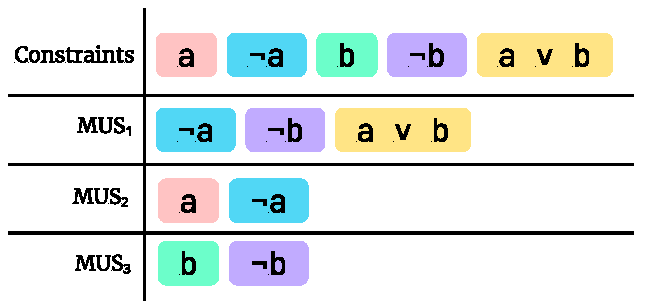
\includegraphics[width=0.8\linewidth]{MUS}
  \caption{
    \label{fig:mus-example}
      An example possible MUSes of a constraint system in propositional logic}
\end{figure}

\subsection{Minimal Correction Subset and Maximally Satisfiable Subset}

Despite the common usage in type inference, MUS is not the only useful subset to representing type error. Minimal correction subset (MCS) can be understood as the smallest subset that needs to be removed to make the rest of the system satisfiable. Formally, a minimal correction set (MCS) $M$ of a constraint system $C$ is a subset $M \subseteq C$ such that $C \setminus M$ is satisfiable and $\forall{S} \subset M : C \setminus S$ is unsatisfiable. MCSes are so named because their removal from $C$ can be seen to “correct” the infeasibility. Because of the property that ``Removing MCS will repair the rest of the system", MCS is effective in representing the cause of error. In an ill-typed program, an MCS can be seen as the smallest set of locations that needs to be modified to fully resolve the type error.  Like a constraint system can have multiple MUSes, MCSes are not unique either. In the example (Fig. \ref{fig:mcs-example}), 4 MCSes can be found. Removing each of these will result in an satisifiable set of constraints. 

\begin{figure}[hbt]
  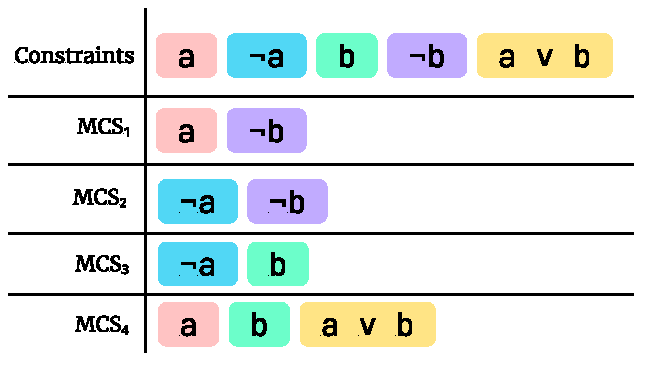
\includegraphics[width=0.8\linewidth]{MCS}
  \caption{
    \label{fig:mcs-example}
      An example possible MCSes of a constraint system in propositional logic}
\end{figure}

The Maximal Satisfiable Subset is the complement of MCS. Formally, a maximal satisfiable subset (MSS) $M$ of a constraint system $C$ is a subset $M \subseteq C$ such that M is satisfiable and $\forall{c}\ in\ C \setminus M:M\cup\{c\}$ is unsatisfiable. The definition of an MSS is symmetric to that of a MUS, with `satisfiable' and `unsatisfiable' swapped along with maximal for minimal. In an ill-typed program, an MSS can be seen as the resulting typing environment if a type error is fixed by relaxing the MCS. An example of MSSes in a constraint system can be seen in Fig \ref{fig:mss-example}.


\begin{figure}[hbt]
  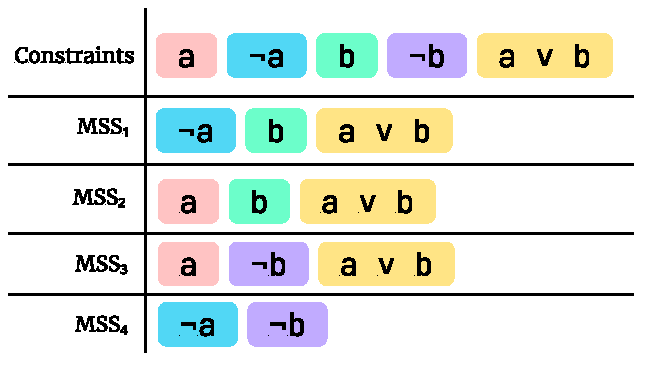
\includegraphics[width=0.8\linewidth]{MSS}
  \caption{
    \label{fig:mss-example}
      An example possible MSSes of a constraint system in propositional logic}
\end{figure}1

\subsection{MUS Enumeration}
 Minimal Unsatisfiable Subsets are often not unique, tt is possible for an unfeasible system to contain a finite number of MUSs. In practice, the existence of multiple MUSes itself is a valuable piece of information. In type checking, it indicates that there are multiple sources of conflict. Enumerating multiple MUS/MCS in this case may provide better insights into the root cause and how to address them properly. We will present an application of enumerating MUS/MCS in Chapter \ref{chap:goanna}.

The problem with MUS enumeration is that it is very computationally expensive. In the most naive approach, it requires exploring the power set of all constraints in the constraint system. In fact, most of the effective enumeration algorithms today rely on heuristics, and they provide performance improvements on a case-by-case basis. MARCO~\cite{Liffiton2016-xi} and MUST~\cite{Bendik2020-pz} are examples of such an approach. They use heuristics to avoid traversing a large chunk of the subsets, each representing a permutation of which constraints need to be relaxed and which do not.


% \begin{figure}[hbt]
%   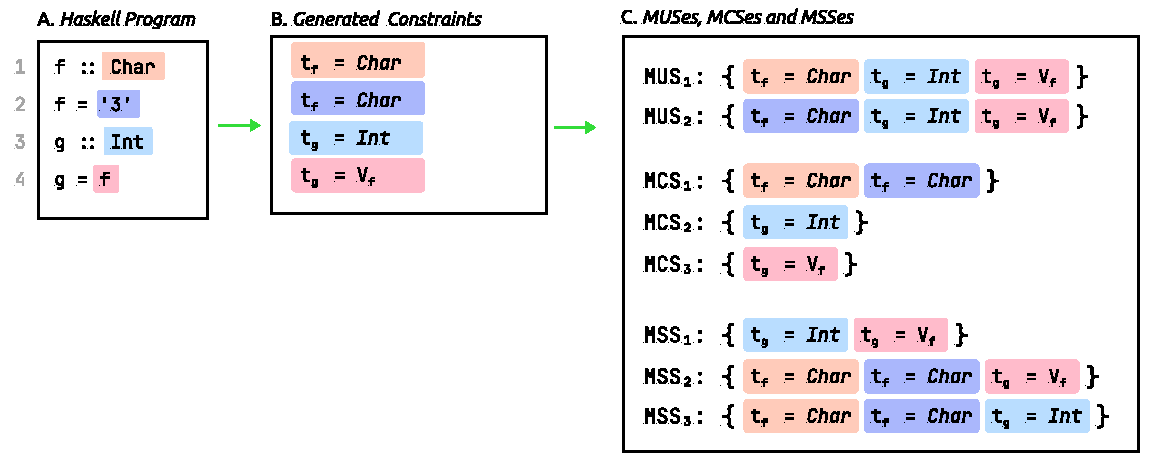
\includegraphics[width=\linewidth]{Subsets}
%   \caption{An example of generating constraints from Haskell program, and all the possible MUSes, MCSes, and MSSes can be acquired.}
% \end{figure}

\section{Three Classes of Type Error}
With the introduction of MUS, we can revisit the idea of three categories of type error we proposed in Chapter \ref{chap:introduction}. This categorization allows a formal study of the tools that is necessary to cover the information of a given type error. 

\subsection{Multi-step Type Error}
\begin{figure}[hbt]

  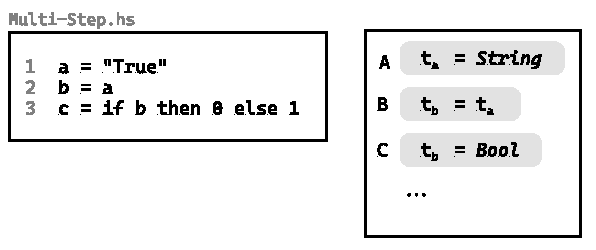
\includegraphics[width=0.5\linewidth]{Multi-Step-2}
  \caption{
    \label{fig:multi-step-2}
    A multi-step type error
  }
\end{figure}
Multiple-step type errors contain a chain of reasoning steps or a series of attempts to unify two logical terms. Multiple step type error contains a single MUS. And each element of the MUS form a singleton MCS. In the example of Fig \ref{fig:multi-step-2}, the MUS is the set of {A, B, C}. The MCSes are {A}, {B}, {C}. Removing any one of the MCS will result in the program type check.

\subsection{Multi-witness Type Error}
\begin{figure}[hbt]
  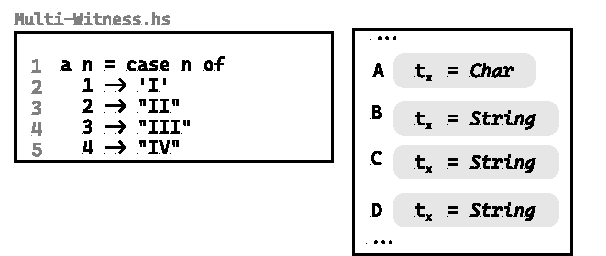
\includegraphics[width=0.5\linewidth]{Multi-Witness-2}
  \caption{
    \label{fig:multi-witness-2}
    A multi-witness type error
  }
\end{figure}

A Multiple-witness type error occurs when one side of the conflict contains multiple locations (witnesses) suggesting the same typing assignment. If one such location is removed, the type error will remain. In the example (\ref{fig:multi-witness-2}), there are three MUSes: {A, B}, {A, C}, {A, D}. Therefore, this type of error cannot be succinctly represented by a single MUS. 

\subsection{Multi-party Type Error}
\begin{figure}[hbt]
  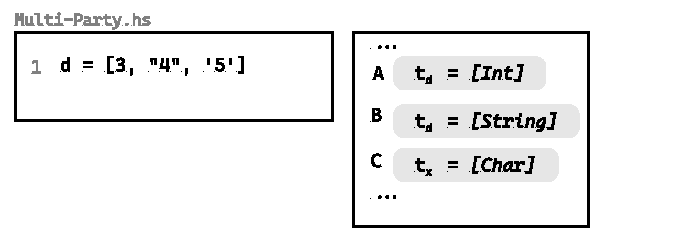
\includegraphics[width=0.5\linewidth]{Multi-Party-2}
  \caption{
    \label{fig:multi-party-2}
    A multi-party type error
  }
\end{figure}

A multiple-party type error is an error where multiple types of irreconcilable assignments can be obtained from locations in the source code. In the provided example  (\ref{fig:multi-party-2}), there are 3 MUS: {A, B}, {A,C}, {B,C}. Therefore, this type of error cannot be succinctly represented by a single MUS.

\begin{figure}[hbt]
  
  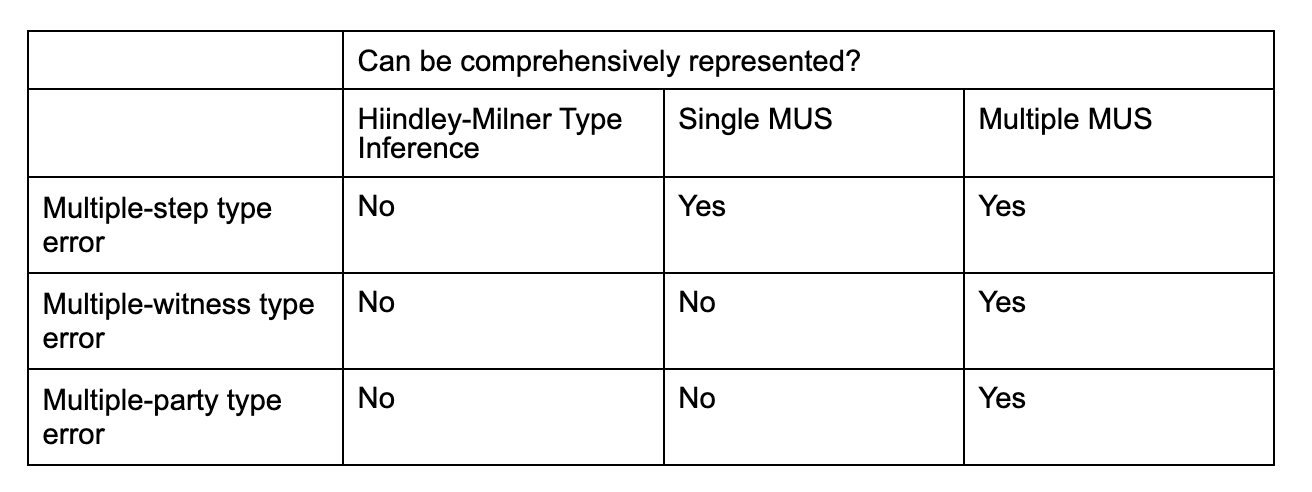
\includegraphics[width=\linewidth]{Compare}
  \caption{}
\end{figure}

\section{Conclusion}
In this chapter, we established a subset of the Haskell language by defining its syntax and typing rules. We explored two avenues to type-check a program in such language and obtain principle types: using the Hindley-Milner type system and using a constraint-based type system. In addition, we explored some type error analysis tools that are enabled by using a constraint-based type system and how these tools are applied to three different kinds of type errors. We will explore them in the next two chapters.
 
\graphicspath{{Figures/Chameleon}}

\chapter{\chameleon{}: Interactive Type Error Exploration}


\label{chap:chameleon} 

In this chapter, we explore the challenges associated with traditional tools for debugging type errors. We focus on their limitations in identifying all relevant locations, explaining errors in user-friendly language, and avoiding bias. We introduce Chameleon, a type error debugging tool for Haskell designed to address these challenges and present type errors in an optimized, comprehensible manner. We delve into the design of Chameleon and demonstrate its usage through examples of resolving type errors. Finally, we present our user studies, which are designed to evaluate the effectiveness of type error visualization and interactive debugging tools.


 This chapter uses the content from our paper \textit{ChameleonIDE: Untangling Type Errors Through Interactive Visualization and
Exploration}, with slight modifications to ensure coherence within this thesis. This work was published and presented at the International Conference on Program Comprehension (ICPC) 2023.



% \todo{As above, would start with motivation of dynamically typed langs e.g. JavaScript, Pythjon popularity but issues this brings...
% }
\section{Introduction}
% Dynamically typed programming languages such as JavaScript and Python have risen in popularity in recent decades \cite{Chatley2019-uq}. These languages present a low barrier of entry, especially to beginner programmers: they require no type declaration, variable types or object structures can be modified dynamically, and functions can deal with dynamic input using ad-hoc polymorphism and runtime reflection. However, studies show that dynamically typed languages negatively affect development productivity \cite{Kleinschmager2012-bg}, code usability \cite{Mayer2012-lg}, and code quality \cite{Gao2017-xn, Ray2017-gq, Meyerovich2013-pn}. They are often found to produce error-prone code \cite{Chen2020-nq, Wang2015-rs, Xu2016-za} and require strong programmer discipline to avoid pitfalls \cite{Chen2020-nq}. For these reasons, many modern dynamically-typed languages have introduced static typing annotations as part of the core language features in recent years (e.g.\ \textit{TypeScript}~\cite{Microsoft_undated-ts} and \textit{mypy}~\cite{Mypy_undated-oe}).

Functional programming languages such as Haskell, and ML have long enjoyed rigorous type systems and expressive type-level features. Techniques such as type inference and algebraic types have been standard practice for decades in these languages, and more recently in multi-paradigm languages, such as Rust and TypeScript. Various type system advances were introduced in Haskell and ended up in mainstream languages years or even decades after, leading many to consider Haskell the ``type-system laboratory" \cite{Hudak2007-kn}.  Type classes, an implementation of generic programming, were introduced to Haskell in 1988~\cite{Hudak2007-kn}, and now can be found in most popular languages such as C\#~\cite{Bill_Wagner2022-sq}, Java~\cite{Oracle2022-lc}, and TypeScript~\cite{Microsoft2022-tl}.

One crucial challenge of programming in Haskell, and many other statically-typed languages, is that type errors can sometimes be difficult to resolve~\cite{Tirronen2015-nr, Hage2020-hg}. In particular, they may point to locations that are not the root  causes of the type error, expose errors in cryptic language, or provide misleading fixing suggestions~\cite{Wu2017-eb}.
% Compared to dynamic type systems, static type systems offer programmers opportunities to weed out a large number of errors at compile time (reducing the need for run-time debugging) and to increase usability~\cite{mayer_static_2012} and codebase maintainability~\cite{kleinschmager_static_2012}. In recent years, the programming community has seen a trend of migrating away from dynamically typed codebases due to the lack of maintainability and refactoring safety when systems reach large scale and complexity~\cite{chatley_next_2019}. These migration methods include the introduction of gradual type annotations (e.g., JavaScript to TypeScript or Python with mypy) or transition to a modern strongly-typed language (Scala, Rust, Haskell, PureScript, etc.). However, with dynamically typed languages (e.g., JavaScript, PHP, and Python) still being most peoples' formative experience with programming and with such languages now firmly entrenched in education~\cite{stackoverflow_stack_2022}, this transition may pose difficulties for programmers who lack experience writing type-safe programs.

% \todo{There are a lot of minor grammer fix-ups needed throughout...}
% Programmers find challenges in adopting typed languages in their practice. \todo{I think this statement is plain wrong myself... 
%  Need strong references to justify if going to say this to SE audience!:}They tend to be verbose, hard to learn and generate bad error messages. 
% One obstacle programmers face when using a statically typed language is understanding and resolving type errors~\cite{marceau_measuring_2011, tirronen_understanding_2015}, especially when dealing with modern type features such as polymorphic types and implicit typing. Studies show most statically typed languages produce unhelpful and even misleading type errors~\cite{}. Symptoms of bad error messages include cryptic language exposing internal constructs of the compiler and incomplete or wrong error locations. These usability issues pose challenges to learners and teachers of the languages. impede the wide adoption of statically typed languages, especially for programmers who are now accustomed to the mindset of writing un-typed programs.

This paper introduces \chameleon{}, an interactive type debugging tool for Haskell. It can visualize the relevant context of a type error: where it happens or could have happened and which parts of the code cause it. In addition, \chameleon{} allows programmers to interactively explore all the parts of code where multiple types can be inferred and to resolve ambiguity. The most noticeable features are the type compare tool (Section~\ref{sub:type-compare}), the candidate expression card (Section~\ref{sub:candidate-expression}), and the deduction step (Section~\ref{sub:deduction-steps}). These features are integrated into a debugging environment and can be enabled or disabled separately based on the programmers' preferences and debugging needs. \chameleon{} is open-source and is available at ~\cite{Fu2022-xp}.  
% \todo{Introduce Haskell earlier?  Motivate WHY Haskell?} The current implementation of \chameleon{} targets the Haskell 2010 language standard. However, it is planned to extend it to support other programming languages using the same underlying ideas and techniques. Historically, Haskell has been a test bed for advanced language features, and it is common for features established in Haskell to be transferred to mainstream programming languages. 

% \chameleon{} uses underlying type inference algorithms adapted from the command-line tool, Chameleon, developed in 2005 \cite{chameleon}. As described in Section~\ref{sec:typeinferenceengine}, Chameleon computes the Minimum Unsatisfiable Subset (MUS) \tf{Explain what mus is} of type constraints in order to identify a set of code locations where multiple types can be inferred. Compared to standard compiler messages, which arbitrarily report the first place a type conflict arises, Chameleon error messages give a lot more context to the programmer to help them correctly resolve the conflict to match the program's intent. However, the Chameleon system was never tested with users.  Therefore, the first contribution of this paper is to address the research question: \textit{Is a minimally interactive version of Chameleon's multipart type-conflict display more effective in supporting type error debugging than traditional error messages? } (Sections~\ref{sub:us1} and \ref{sub:us2}).

% After affirming that the information Chameleon provides is beneficial for more complex type errors, we ask \textit{Do programmers benefit from the interactive exploration of type error locations?} (Sections~\ref{sub:us3} and \ref{sub:us4}). We then explore \textit{How do programmers use the interactive exploration features to solve type errors?}  (Section~\ref{sub:us4}).


This paper makes the following contributions:
\begin{itemize}
\item We provide the design and implementation of the \chameleon{} to visualize the relevant context of a type error and allow programmers to explore and verify the error locations in small chunks interactively.  
\item {
    We report the results of three experiments designed to evaluate \chameleon{}.}
\end{itemize}

Our experiments showed that programmers using \chameleon{} fix type errors faster than with traditional text-based error messages. This difference is more significant when solving harder tasks. Further, programmers who actively use \chameleon{} interactive features fix type errors faster than simply reading the type error output. Although \chameleon{} is designed to work with
the Haskell language, we plan to extend the underlying ideas to work with other strongly typed languages, such as Rust or TypeScript..

\section{Motivation}
The design requirements of \chameleon{} are motivated by limitations of traditional type errors, as documented in a number of studies (e.g.~\cite{Yang2000-wn, Hage2020-hg}), but which we illustrate here with a few motivating examples. 
%These limitations are sourced from the authors' frustration in teaching and writing Haskell. This list of shortcomings of traditional type errors is also strengthened by multiple studies pursuing improvement\cite{yang_improved_2000}. 

\begin{figure}[ht]
    \centering
    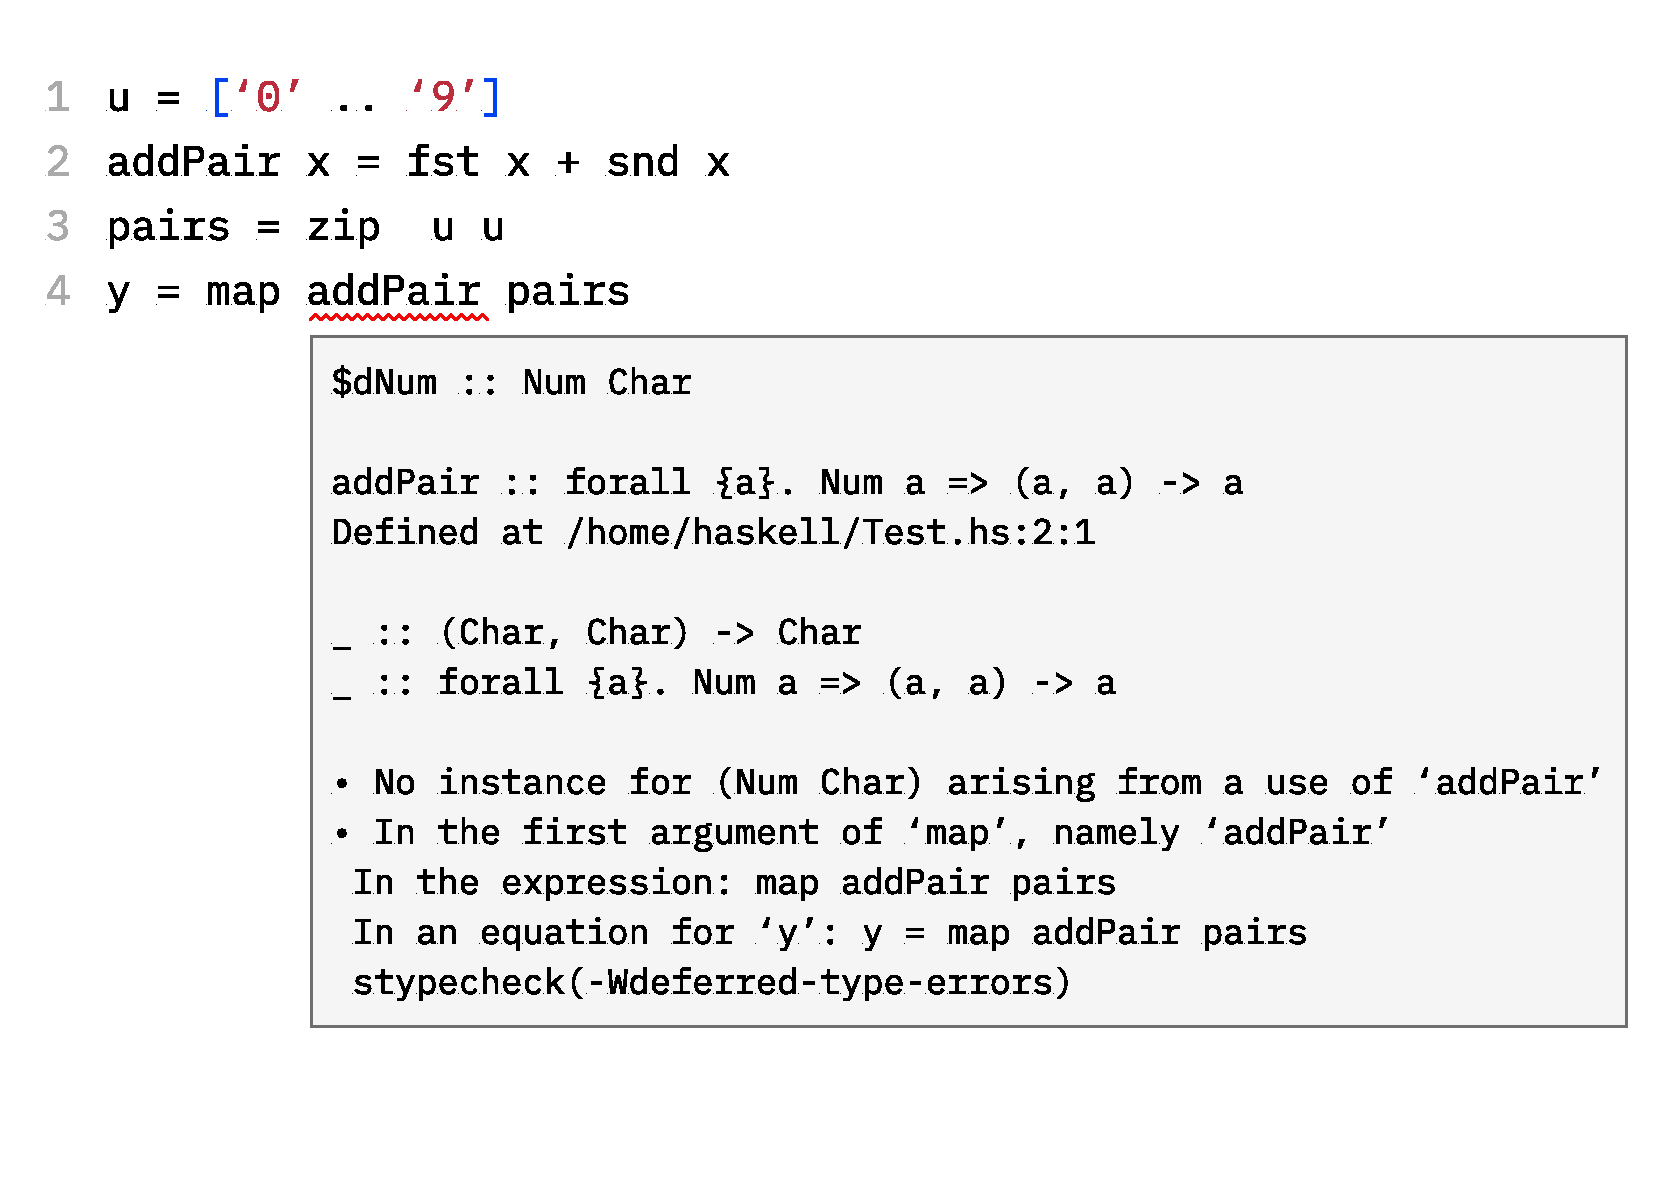
\includegraphics[width=\linewidth,trim=0mm 35mm 0mm 0mm]{images/add-pair-example.pdf}
    \caption[A type error displayed in Visual Studio Code and the Haskell Vscode extension]{
    A type error is displayed in Visual Studio Code\cite{Microsoft_undated-hs} with the Haskell Language Server\cite{HLS-Developers2023-ot} support.
The expression \texttt{addPair} is blamed for causing the type error. This may not match the programmers' intention. 
    }
    \label{fig:motivation-example}
\end{figure}

\textbf{Traditional type errors show only limited location}
Haack and Wells~\cite{Haack2004-fr} noted that ``\textit{Identifying only one node or subtree of the program as the error location makes it difficult for programmers to understand type errors. To choose the correct place to fix a type error, the programmer must find all the other program points that participate in the error.}'' The type error in Fig.~\ref{fig:motivation-example} can be fixed in multiple locations. For instance  replacing \texttt{['0'..'9']} on line 1 with \texttt{[0..9]}, or replacing \texttt{fst x} and \texttt{snd x} on line 2 with \texttt {read (fst x)} and \texttt{read (snd  x)}. In the type error message, only the \texttt{addPair} expression on line 4 was blamed.  The whole context is visible in this small example, but it can become problematic in large programs where the lines contributing to the type error are far apart in the source code.

\textbf{Traditional type errors are biased}
A common form of bias happens when a type error is reported in one expression, but it can occur in multiple other expressions as well. In Fig.~\ref{fig:motivation-example}, the error message arbitrarily focuses on only \texttt{addPair}, while ignoring that the literals in the definition of \texttt{u} may be incorrect. %Technically, this results from the side effect of different unification orders of the internal type-checking technique and has no bearing on what the programmers think and expect. 
Another form of bias is that traditional type errors are often framed as conflicts between \texttt{Expected type} and \texttt{Actual type}. This framing is standard practice in most typed languages. However, what is \texttt{expected} and what is \texttt{actual} are a side effect of different unification orders rather than the intention of the programmer. In both forms, the error message may lead programmers to falsely believe the validity of parts of code and wrongly accuse others.

\textbf{Traditional type errors give poor explanations}

When the compiler type checks a program, it generates a series of constraints from the source code and searches for a model that satisfies all these constraints. However, the details of this process are hard to explain to users and are usually not reported by compilers. For the typical type error shown in Fig.~\ref{fig:motivation-example}, the evidence for the type error is gathered from the previous declarations. These have to be rediscovered by programmers using less rigorous methods. 

\subsection{Design Goals of \chameleon{}}
Based on the limitations of traditional type errors, we give the following design requirements for \chameleon{}:

\noindent\textbf{Show} all the possible locations where the type error happened or could have happened.

\noindent\textbf{Explain} type errors, avoiding jargon and internal constructs of the type checker.

\noindent\textbf{Do not presume} which expression is to blame for the type error based on the order of computation or which possible type for an expression is `actual' or `expected'.


\section{Chameleon IDE} \label{chameleon}
\begin{figure}[ht]
    \centering
    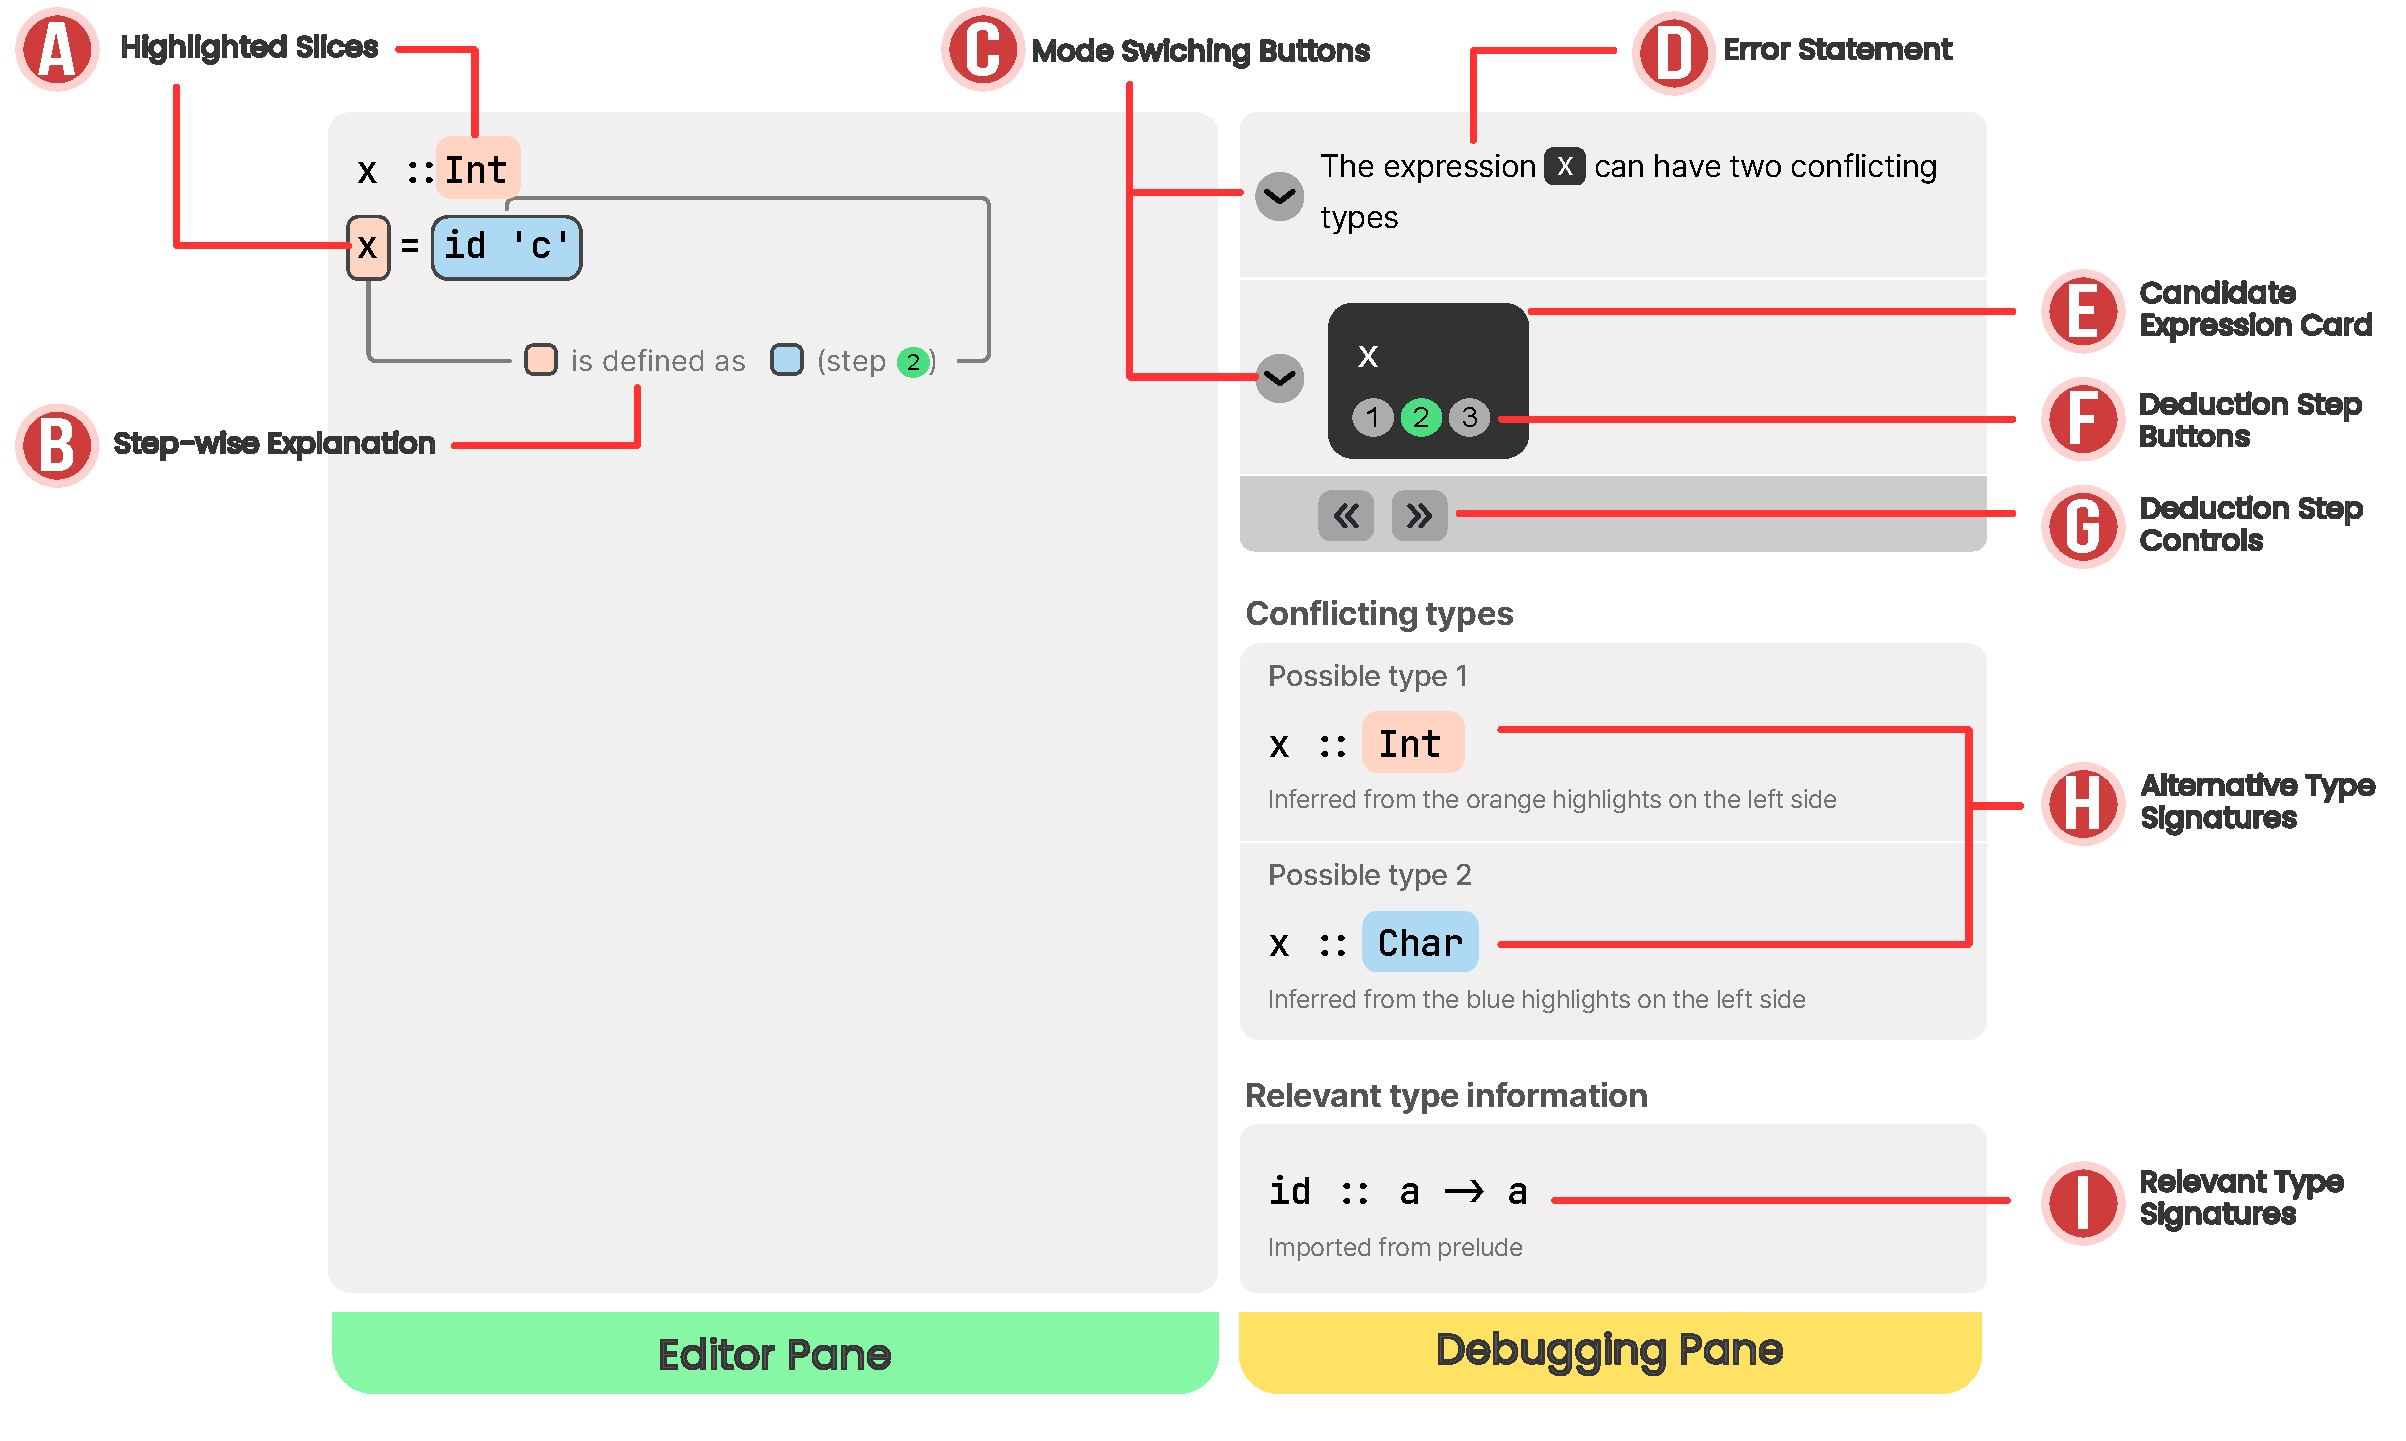
\includegraphics[width=\textwidth, trim=0mm 10mm 0mm 0mm]{images/atonomy.pdf}
    \caption[The anatomy of \chameleon{}]{
        \textbf{The anatomy of \chameleon{}.}
        The editor pane (left) is similar to a traditional code editor. Fragments of source code may have a highlight
        color (A). Additionally, an explanation layer (B) displays if deduction steps are enabled. The debugging pane contains three blocks. First, the error statement block contains an error statement (D), optionally, a list of candidate expression cards (E), a list of deduction steps (F), and a control bar (G) to increment/decrement deduction step. Second, the conflicting types block shows two alternative types (H). Third, the relevant type information block shows additional information (I) that may help understand type errors.
    }
    \label{fig:anatomy}
\end{figure}


\chameleon{} comprises two parts: a type inference engine and a novel interactive debugging interface. 
% This separation of concerns allows us to (1) adapt \chameleon{} into multiple front ends, such as IDE extensions, desktop applications, and web applications; and (2) reuse the debugging interface for different programming languages by replacing the back-end type inference engine. 
The debugging interface is designed from the ground up; the type inference engine is a re-implementation of the original Chameleon with several novel improvements, as described in Section~\ref{sec:typeinferenceengine}.

% \todo{I wonder about a high level overview diagram of tool / usage of tool, then the details of each component?}

% \todo{Can you use this example in Motivating Example sectoon (see my comment above) then use it to explain tool in this section?  Make sense?

% Is this example too simple...?}

\subsection{The Debugging Interface}

The \chameleon{} debugging interface provides three main features to visualize and explain type errors.

% the relation between the error statement and locations in code and to explore the explanation of each error location given by the type inference engine. 
%Further, programmers  can turn on and off features to suit their preferences and debugging needs.


\paragraph{Type compare tool} \label{sub:type-compare}
% In designing \chameleon{}, we want to argue against the practice of reporting type errors as the conflicts between \texttt{Expected type} and \texttt{Actual type}. Technically, the two alternatives are merely the side effect of different unification orders of the internal type-checking technique and have no bearing on what the programmers think and expect. 

The type compare tool shows conflicting types in different colors, each type associated with one or more error locations highlighted in a matching color (Fig.~\ref{fig:compare}).  
%The type error must be fixed by modifying at least one of these locations. 
%Error locations are highlighted with the matching color of the conflicting types. The type compare tool is useful to quickly bisect the type error. 
If the programmers know the expression's intended type (they usually do), they will be able to eliminate half of the possible locations. 
%To make this bisecting effect more pronounced, a user can hover over one of the possible types and only show the relevant locations that contribute to that type. 
A hover interaction over one of the possible types facilitates such bisection, causing only the relevant locations that contribute to that type to be highlighted. 
%This is a convenient way to put the error \emph{under the spotlight}.


\begin{figure}[ht]
    \centering
    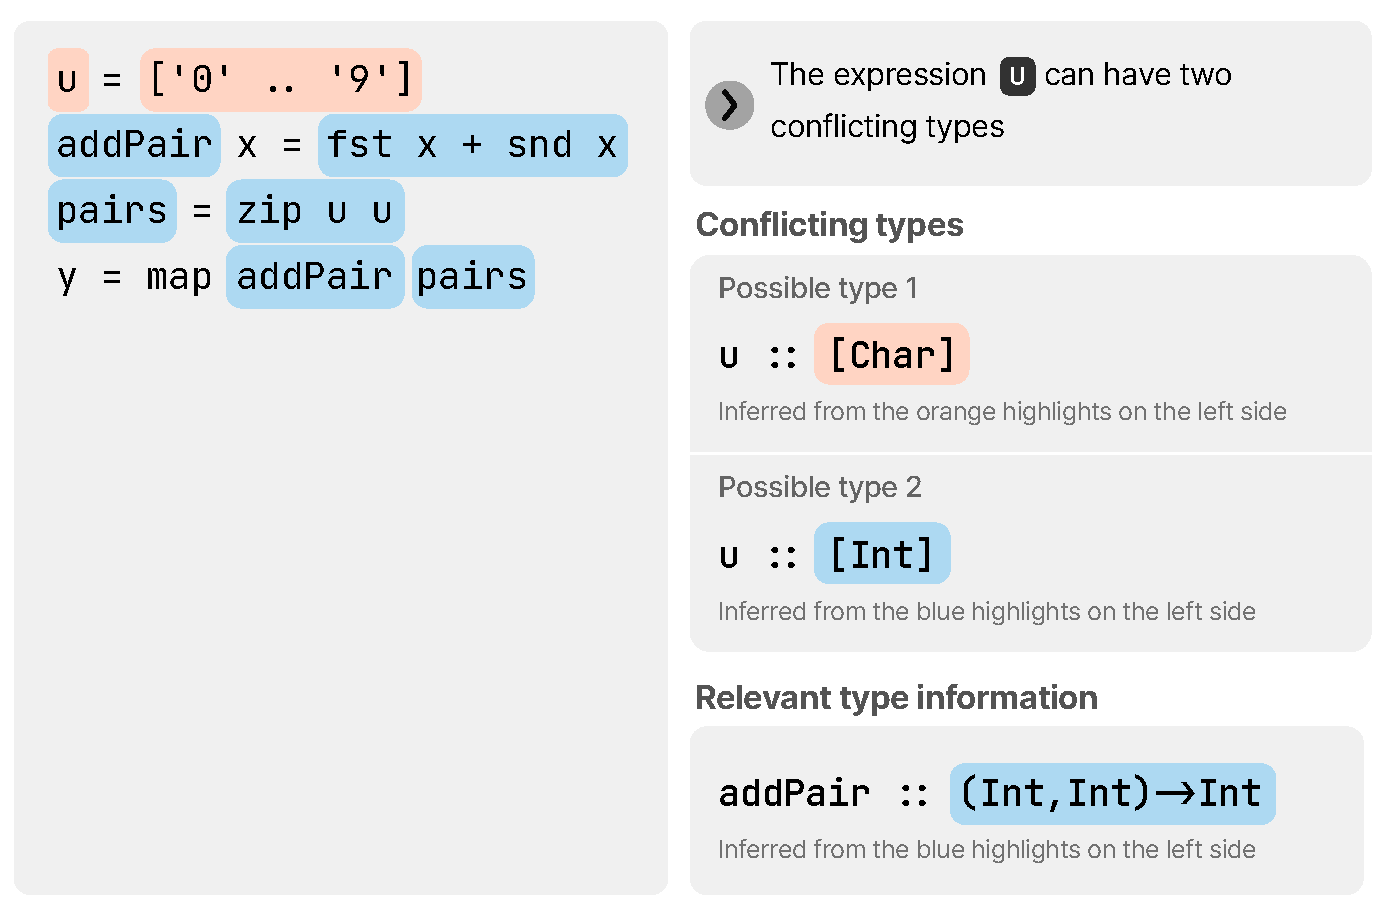
\includegraphics[width=\linewidth, trim=0mm 10mm 0mm 0mm]{images/intro-compare-2.pdf}
    \caption[\chameleon{} with type compare tool enabled]{
        \textbf{\chameleon{} with type compare tool enabled}. \chameleon{} identified the conflicting types for the expression \texttt{u} and associated the relevant locations with each type. Compare the output with the traditional type error message in Fig.~\ref{fig:motivation-example}.
}
    \label{fig:compare}
\end{figure}

\begin{figure}[ht]
    \centering
    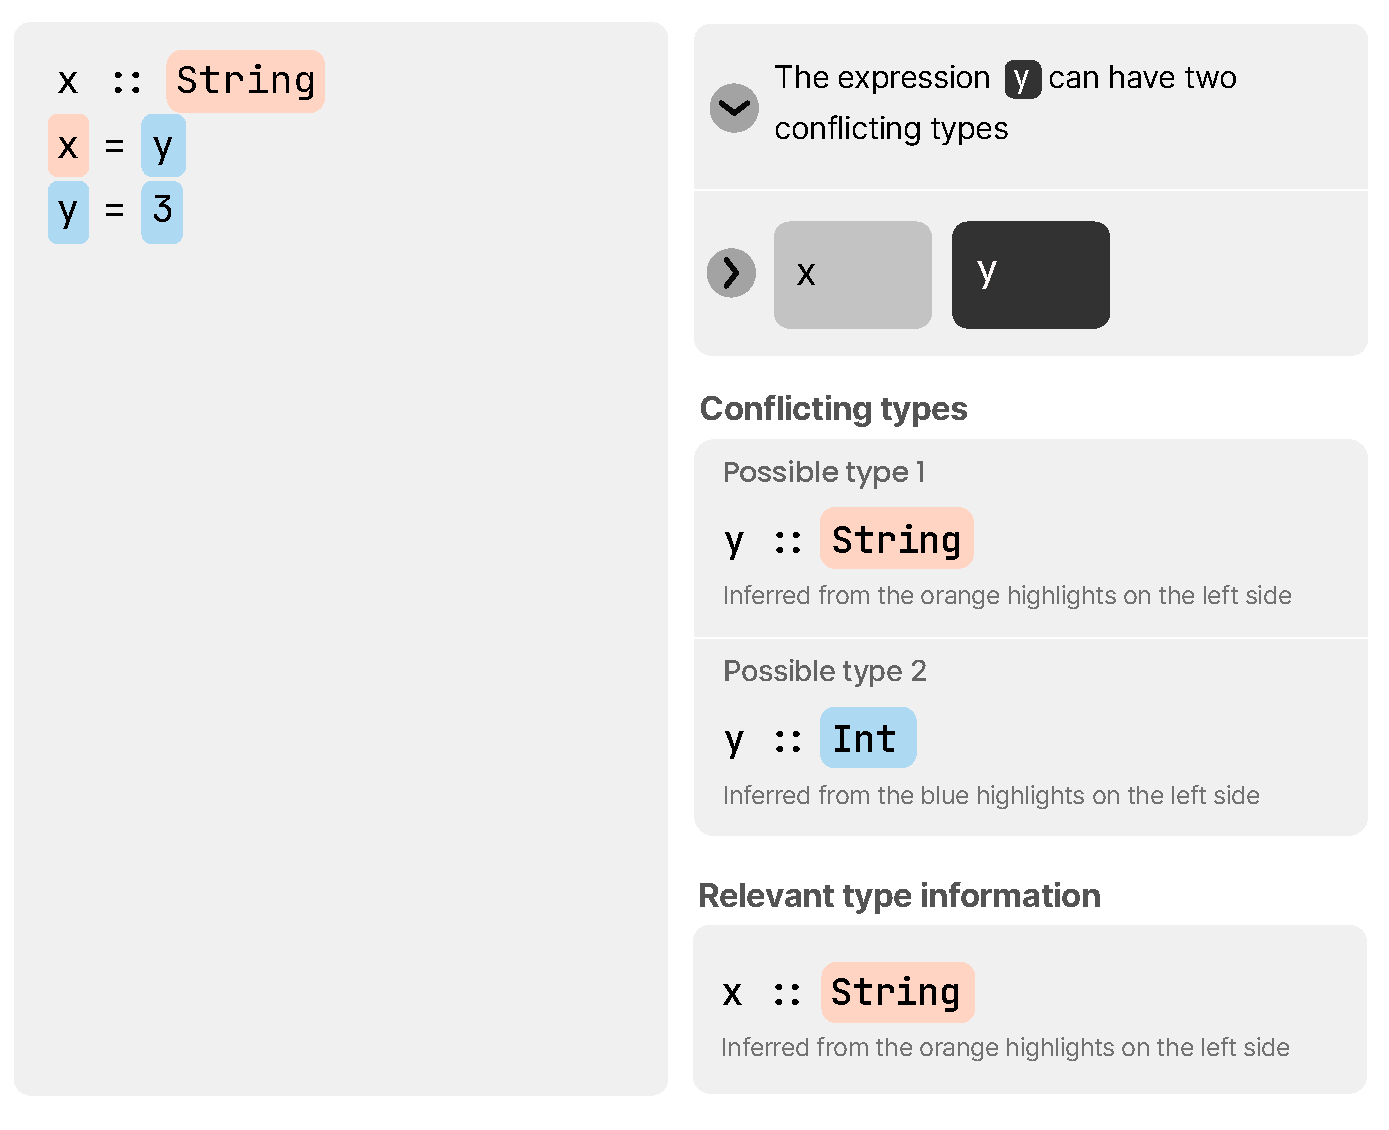
\includegraphics[width=\linewidth, trim=0mm 10mm 0mm 0mm]{images/intro-candidate.pdf}
    \caption[\chameleon{} with candidate expression cards enabled.]{
        \textbf{\chameleon{} with candidate expression cards enabled.}
        Indicates the type error can occur in the definition of \texttt{x} or \texttt{y}.
    }
    \label{fig:expression}
\end{figure}


\begin{figure}[ht]
    \centering
    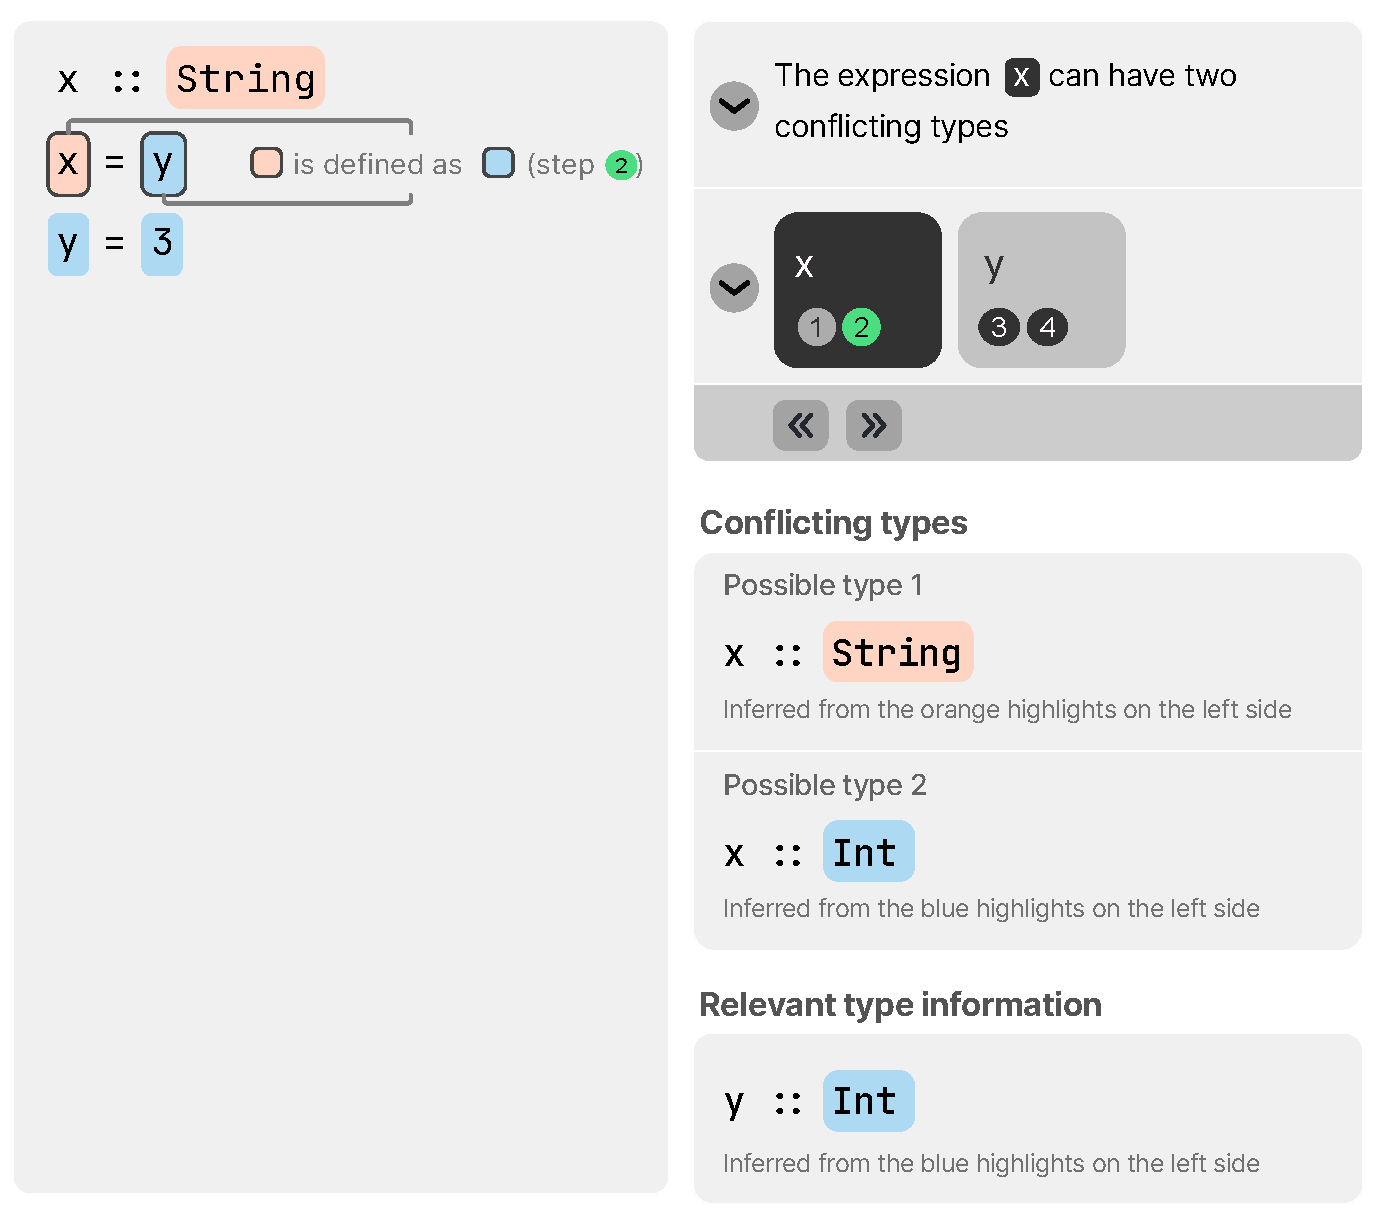
\includegraphics[width=\linewidth, trim=0mm 10mm 0mm 0mm]{images/intro-deduction.pdf}
    \caption[\chameleon{} with deduction steps enabled]{
        \textbf{\chameleon{} with deduction steps enabled.}
        \chameleon{} explains the type error in four steps. In the screenshot, the active step is step 2, where \chameleon{} shows that the expression \texttt{x} and \texttt{y} should have the same type. 
    }
    \label{fig:deduction}
\end{figure}



\paragraph{Candidate Expression Cards}  \label{sub:candidate-expression}


% We propose candidate expression cards to make it clear to the user that there are multiple ways to resolve a type conflict. By contrast,  standard compiler error messages such as those of GHC arbitrarily focus the users' attention on only one candidate expression, e.g.\ ``\textit{Couldn't match expected type ‘Char’ with actual type ‘Bool’ in expression x}" where x is the candidate expression. In practice, this candidate expression often does not match programmers' intention (Fig.~\ref{fig:single-candidate}).  
A candidate expression is an expression that can be inferred to have two conflicting types. 
When a type error is detected, \chameleon{} provides a list of all candidate expressions, and programmers are free to choose the problem to resolve by clicking on one candidate expression card. In the example shown in Fig.~\ref{fig:expression}, \texttt{x} and \texttt{y} are both candidate expressions. Fixing either type error can make both expressions well-typed.


% This feature can be effective in resolving the problem that traditional tools tend to report errors that happened in source code from third-party libraries. With candidate expression cards, a programmer can freely change the context of the type error to the user-defined variables and functions to gain a better understanding of why their own code does not match the library code instead of the other direction.


Programmers select a candidate expression card by clicking on one card. Once a card is selected, the information in the conflicting types block changes to reflect the change of candidate expression. In the editor pane, some error locations change highlight colors based on the updated candidate expression. Alternatively, programmers can preview the change of a candidate expression by hovering on one card. The hover effect is reverted once the cursor moves away. 


\paragraph{Deduction steps}  \label{sub:deduction-steps}

% Deduction steps are motivated by the lack of explaining why the program has type errors. When the compiler rejects a program, it dumps the internal state of type checking.  This information may be a result of complex computing but this process is not reported by compilers. For a typical type error shown in Fig.~\ref{fig:ghc-error-example}, clearly, the evidence for the type error is gathered from the previous two declarations. These have to be rediscovered by the programmers again, using harder and less-sound methods. 

% \begin{figure}
%     \centering
%     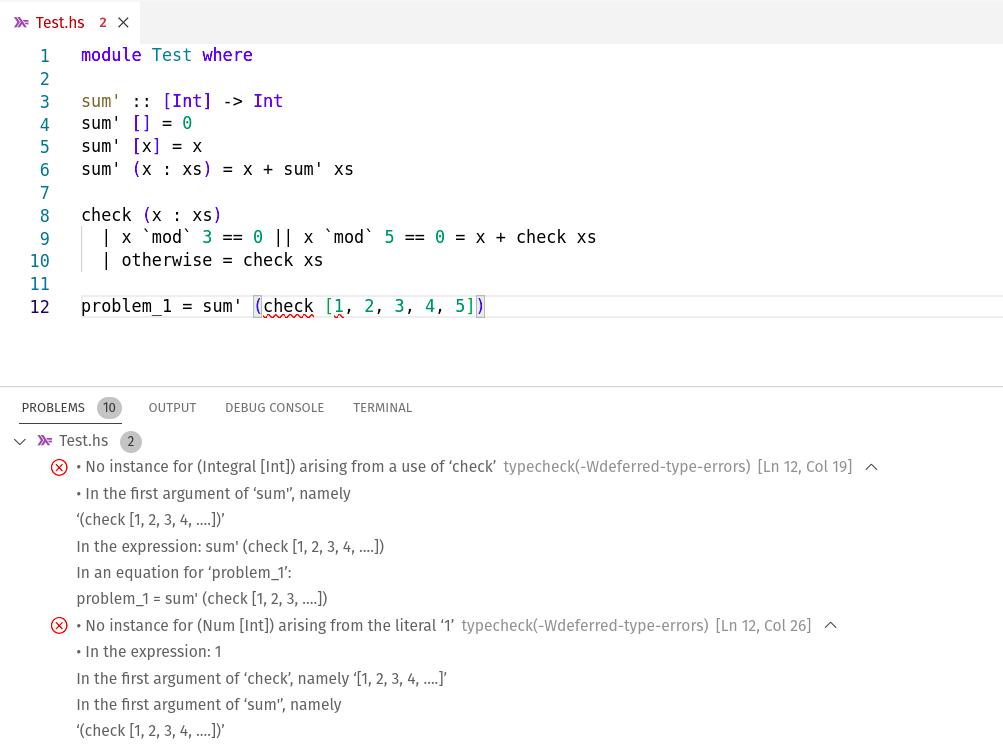
\includegraphics[width=\linewidth]{images/ghc-error-example.png}
%     \caption{
%         }
%     \label{fig:ghc-error-example}
% \end{figure}

Deduction steps allow programmers to explore all the error locations one at a time (Fig.~\ref{fig:deduction}). Steps are shown as a list of sequentially numbered circular buttons (step buttons) and an explanation layer in the editor window. In the explanation layer, the two locations under examination are outlined, and a line is drawn to connect these two locations. This line is accompanied by a human-readable text explanation of their semantic connection. Programmers are free to activate any step. The active step is shown in green. When activating a step, some highlights switch color. The message in the explanation layer changes accordingly. A program in Fig.~\ref{fig:deduction} generates a list of steps shown in Fig.~\ref{fig:step-interface} left.


Programmers can use mouse and keyboard shortcuts to increment or decrement the step number or jump to any step. Programmers resolve type errors by navigating through all the deduction steps and verifying whether each explanation aligns with their intention. Eventually, they will find a step that does not match, and the type error can be fixed by modifying one of the two outlined locations.

\begin{figure}[ht]
    \centering
    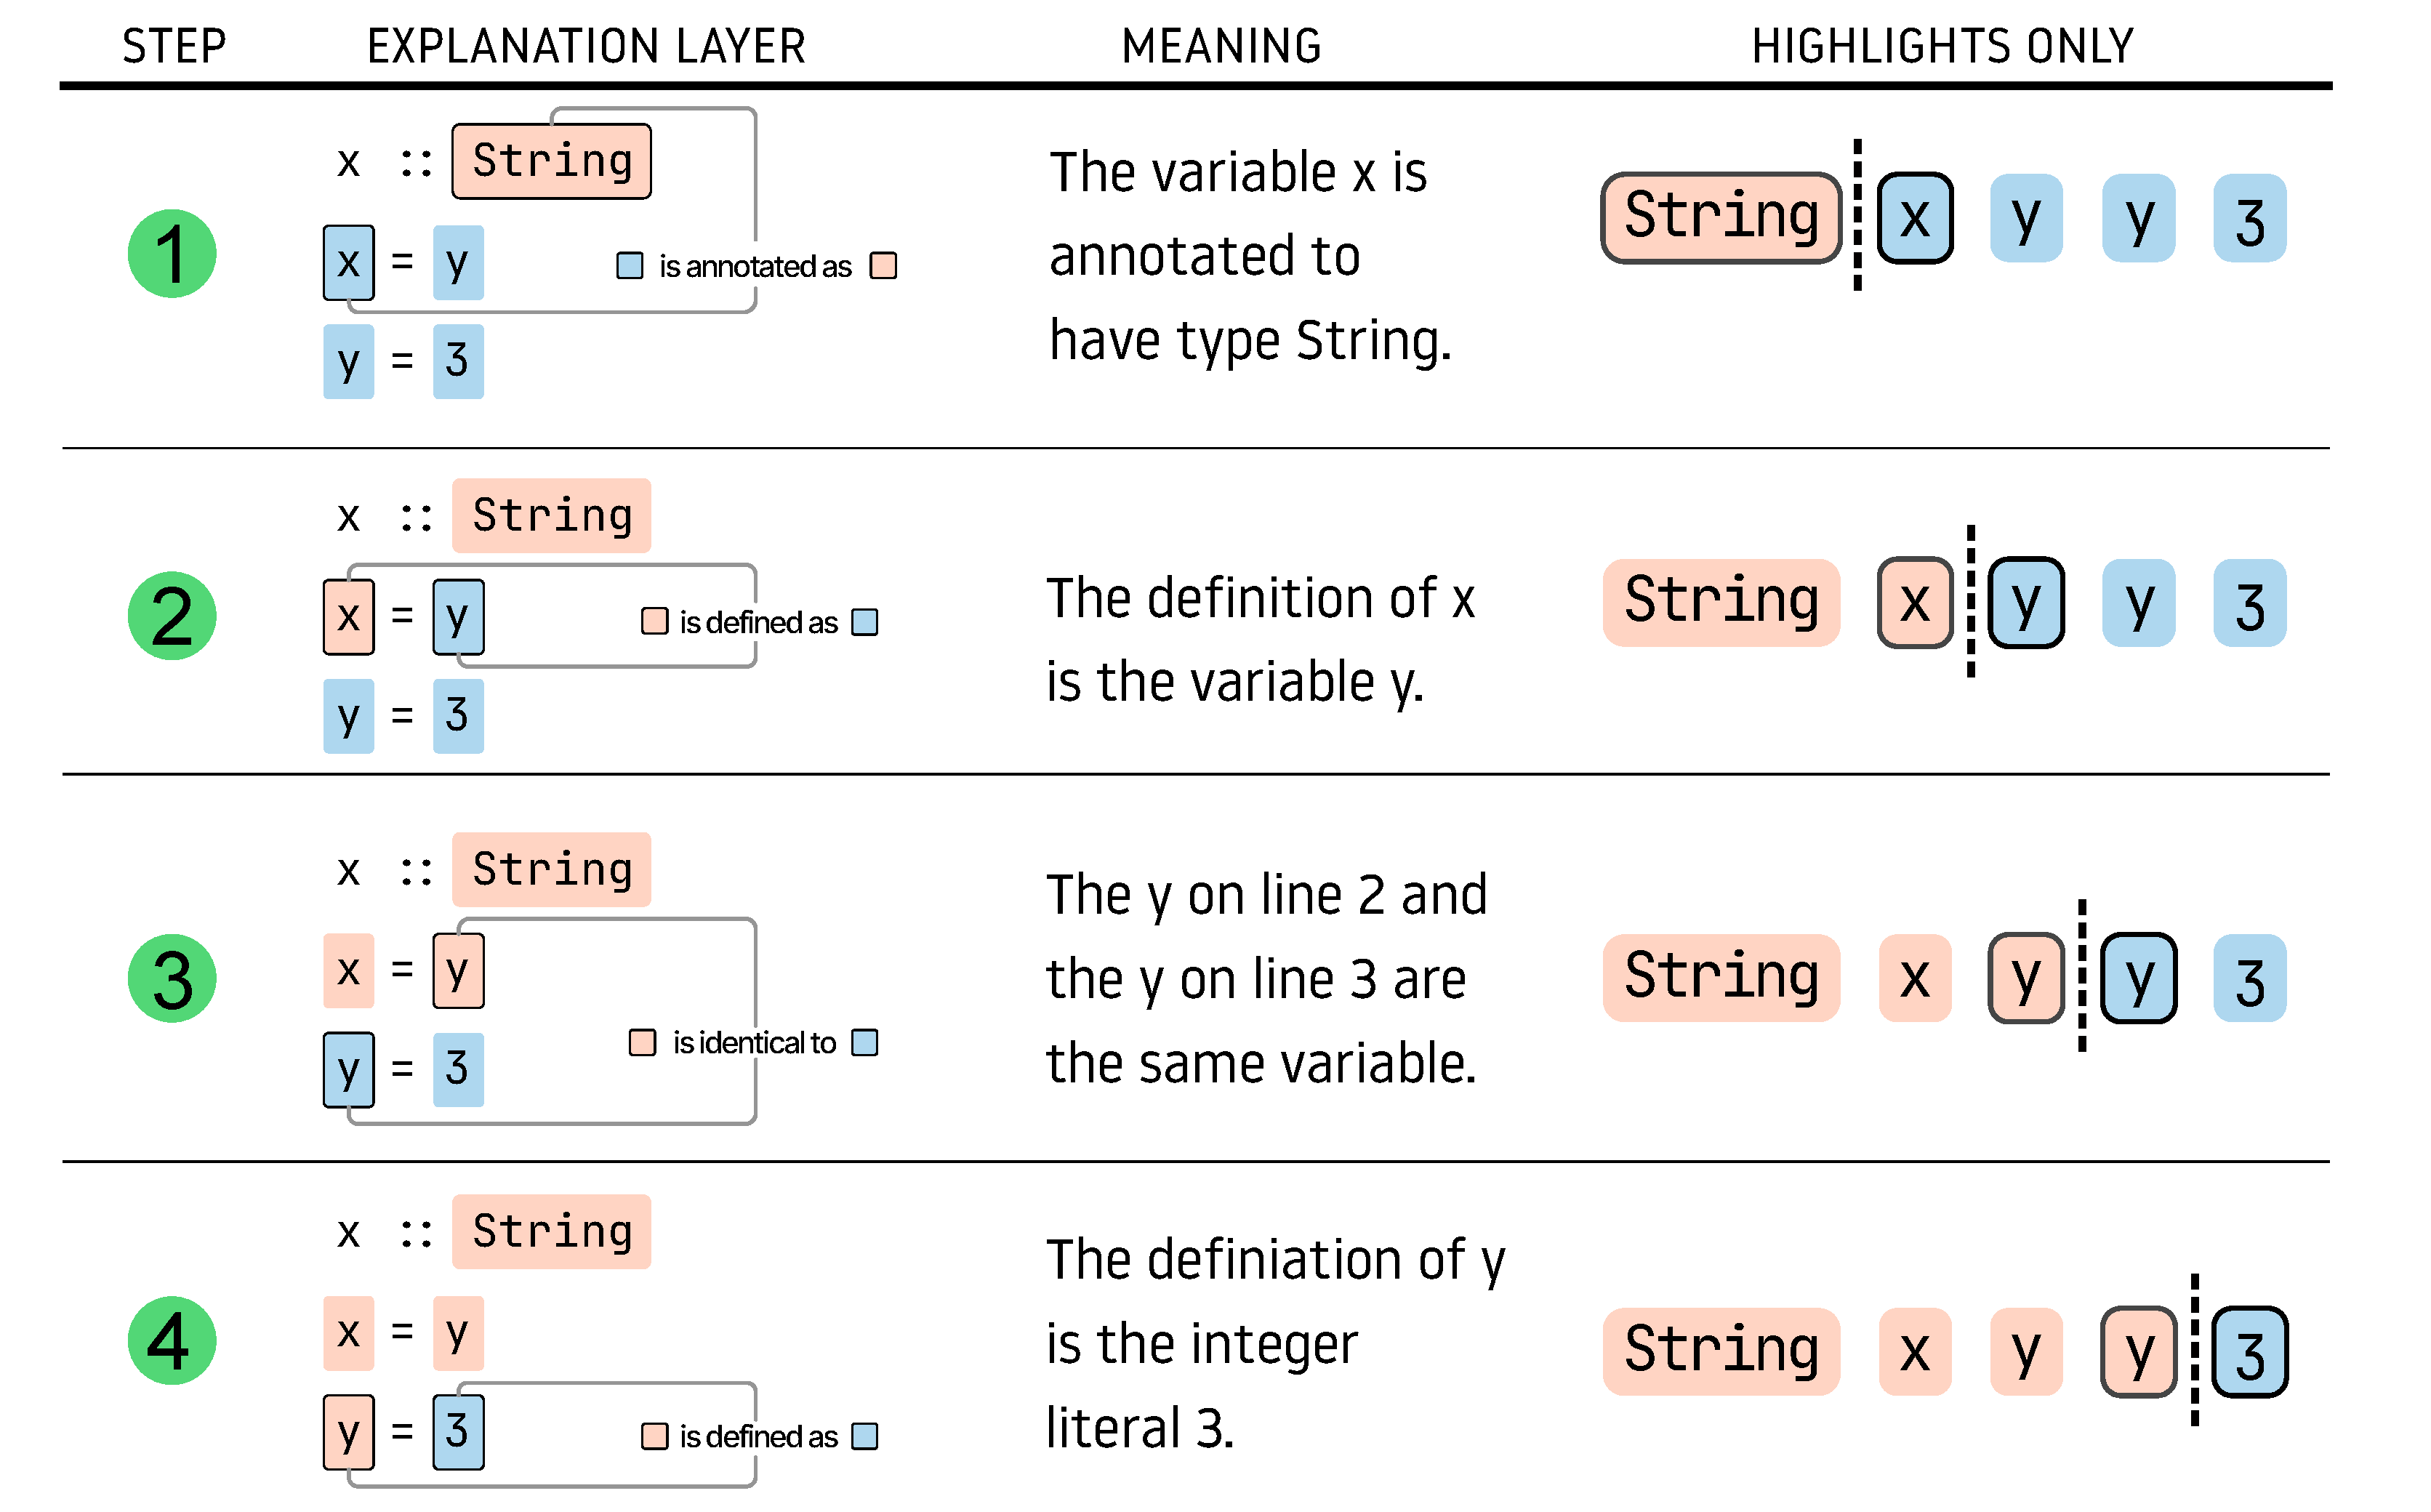
\includegraphics[width=\linewidth, trim=0mm 0mm 0mm 0mm]{images/step-explain.pdf}
    \caption[Deduction steps if they are shown all at once]{
Deduction steps if they are shown all at once. In practice, steps are shown one at a time. Programmers increment or decrement the step number using the step control bar (Fig.~\ref{fig:anatomy}-G) or by directly clicking on a step button (Fig.~\ref{fig:anatomy}-F). To increment or decrement the deduction step can be intuitively thought of as moving the position of the \textit{splitting point} (dotted lines) where the blue and orange highlights divide.
        }
    \label{fig:step-interface}
\end{figure}

Internally, deduction steps are different ways to divide the error locations into two groups, denoted by the two colors. Each color infers a different type of candidate expression. Each increment/decrement of the step changes the splitting point (dotted lines in Fig.~\ref{fig:step-interface}) of the two colors. Deduction steps are an interactive view of multi-step type errors.


\paragraph{Multiple Modes}

Nielson pointed out that the two most important issues in designing for usability are understanding the users' tasks and the differences in users \cite{Jakob_Nielsen1994-gd}. From analyzing how users use \chameleon{}, we realized that the ideal debugging interface should adapt to the specific programmer and programming task. There are cases where a programmer wants the debugger to simply ``show the answer", and others to dive deeper into the problem domain and search for the optimal solution. To accommodate the need to customize the level of information density and granularity of control, \chameleon{} provides three modes: basic, balanced, and advanced. Programmers can switch between modes by clicking on the mode switching toggles (Fig.~\ref{fig:anatomy}-C). The features accessible from different modes are summarized in Table~\ref{tab:chameleon-features}.%shown in table~\ref{tab:chameleon-features}.

\begin{table}
    \centering
\begin{scriptsize}
\begin{center}

    \begin{tabular}{ l l }
     \textit{Mode} & \textit{Features} \\ \hline
     Basic Mode  & Type Compare Tool \\ \hline
     Balanced mode & Type Compare Tool  \\
     & Candidate Expression Cards  \\  \hline
     Advanced mode & Type Compare Tool  \\
     & Candidate Expression Cards \\
     & Deduction Steps  \\
    \end{tabular}
    \end{center}
\end{scriptsize}
    \caption{\chameleon{} modes and features}
    \label {tab:chameleon-features}
\end{table}


\subsection{The Type Inference Engine}
\label{sec:typeinferenceengine}

Chameleon was originally a command-line tool developed in the early 2000s to improve type error reporting %and introduced a design for interactive type debugging 
for the Haskell programming language.
Unlike traditional type errors produced by the Glasgow Haskell Compiler (GHC)~\cite{Gamari_undated-zu}, which uses a Hindley–Milner type inference system, Chameleon infers types using constraint solving. In Chameleon, constraints are generated from the source code based on typing rules. In addition, each constraint is labeled with the location where it is generated. This set of constraints is consistent if the program is well-typed and inconsistent otherwise. When a type error occurs, an efficient algorithm is used to derive a minimal subset of the constraints that still contain inconsistencies. This subset is called a Minimal Unsatisfiable Subset (MUS). From this, Chameleon can report a list of locations, using the labels of constraints that are in the MUS. Stuckey, Sulzmann and Wazny showed that program locations linked to the constraints from an MUS are all relevant to the type error and must include the cause of the error~\cite{Stuckey2003-pz}.

Despite successfully borrowing the underlying ideas, we could not reuse the original implementation of Chameleon since the project language standard and libraries used were out of date. 
\chameleon{} implementation extends the original Chameleon approach in a number of ways. \chameleon{} supports the base language of Haskell2010~\cite{Simon_Marlow2010-lg}. However, \chameleon{} does not support any advanced language extensions, such as GADTs.
%In addition to what Chameleon can do, a few new type inference features were added in the \chameleon{} implementation.



\paragraph{Recovering concrete types from type errors}


Using only constraints from the MUS is sufficient to locate the type error, but to recover types from type errors, we need constraints from parts of the program that are irrelevant to the type error.  For instance, consider an ill-typed 2-tuple where two possible types can be assigned: \texttt{(Int, Int)} and \texttt{(Int, String)}. The types reconstructed from Chameleon may be \texttt{(a, Int)} and \texttt{(a, String)}. Although the recovered types are theoretically correct, they introduce the notation \texttt{a}, which denotes a generic type variable that can be any type, making the error message harder to understand. To solve this issue in \chameleon{}, for each constraint \texttt{c} in the MUS, we find a maximally satisfiable subset (MSS) from all the constraints that contain every other element of MUS but not \texttt{c}. These maximally satisfiable subsets, while not helpful in error localization, will produce the most concrete types, see Fig.~\ref{fig:compare-to-original}. Concrete types, such as \texttt{Int} and \texttt{String},  often provide extra information to programmers. With a type of \texttt{(Float, Float)}, programmers may want to convey a point in 2D space. However, a type of \texttt{(a, Float)} does not preserve such information.


\begin{figure}[ht]
    \centering
    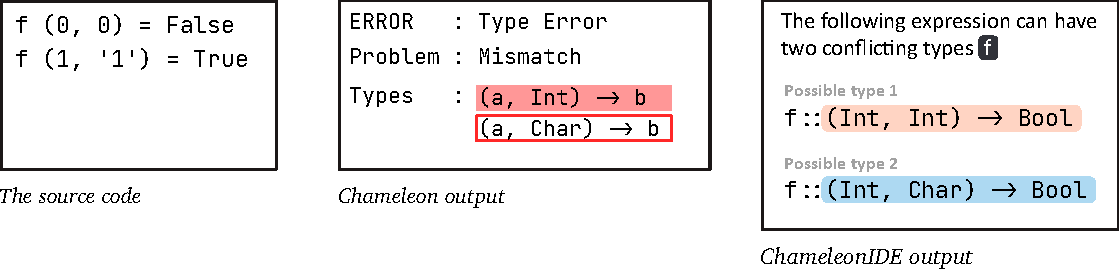
\includegraphics[width=\linewidth, trim=0mm 6mm 0mm 0mm]{images/compare-to-original.pdf}
    \caption[Comparison between original Chameleon and \chameleon{}]{
Reporting the same type error, Chameleon uses more abstract types
\texttt{Int -> a} and \texttt{Char -> a}, while \chameleon{} uses the 
concrete types (types that do not contain type variables) \texttt{Int -> Bool} and \texttt{Char -> Bool}.
    }
    \label{fig:compare-to-original}
\end{figure}

 
% If the types get too verbose for programmers to identify the conflict between the two signatures, it is always possible to mute the overlapping information and highlight the differences from the debugging front end.


\paragraph{Type error explanation}

In addition, \chameleon{} provides support for type explanation. Similar to the type explanation system in ~\cite{Jun2002-xp},  \chameleon{} is able to produce a human-readable explanation, but for type errors. This is achieved by annotating nodes in the abstract syntax tree with constraints and the type inference rules used. We generate an inference history from constraints and accompanying annotations. 


% \begin{lstlisting} [
%     language=Haskell, caption={
%     A simple program that is ill-typed. This program generates two constraints from line 1 and one constraint from line 2.
% }, label={listing:ifelse}
% ]
% if a then b else c
% a = "True"
% \end{lstlisting}


\begin{figure}[ht]
    \centering
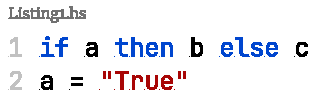
\includegraphics[width=0.4\linewidth]{images/Listing1.pdf}
    \caption[An example to illustrate constraint generation in \chameleon{}]{A simple program that is ill-typed. It generates two constraints from line 1 and one constraint from line 2. }
    \label{fig:listing1}
\end{figure}

For instance, for the program in Fig.~\ref{fig:listing1}, \chameleon{}  generates the following constraints and labels (in brackets) $T_a = Bool$ (if condition), $T_b = T_c$ (if branches), $T_a= String$  (definition). Clearly, as $T_a$ can not unify with both \textit{Bool} and \textit{String}, this program is not well typed. \chameleon{} can construct a human-readable explanation from the MUS. An example output for Fig.~\ref{fig:listing1} can be: \texttt{a} has type \texttt{Bool} because \texttt{a} is the condition of an if statement; however, \texttt{a} has type \texttt{String} because \texttt{a} is defined as the string literal \texttt{"True"}. This explanation facilitates the deduction steps (Section~\ref{sub:deduction-steps}). 







\section{Walkthrough} \label{sec:walkthrough}
In this section, we showcase \chameleon{} by walking through examples of its
use. The examples are given from the perspective of a hypothetical Haskell 
programmer Maxine. 

% \todo{A bit of redundant/repeated here c.f. prev section - if this is Usage example, again use motivating example in it?}

\subsection{Basic mode} \label{sub:basic}
Maxine writes a function to calculate the sum of a list of
numbers, but \chameleon{} shows there is a type error (Fig.~\ref{fig:basic-mode-1}). 
After reading the error reports, Maxine realizes that the error revolves 
around the expression \texttt{xs}. That is: \texttt{xs} can be
either \texttt{[a]} or \texttt{Int}. By matching the color in the
conflicting type block (Fig. \ref{fig:anatomy}-H) and the highlighted error locations 
Maxine knows that the \texttt{[a]} results from the pattern matching of the
\texttt{:} operator, while \texttt{Int} results from using \texttt{+} to
 add two expressions. 

\begin{figure}
        \centering
        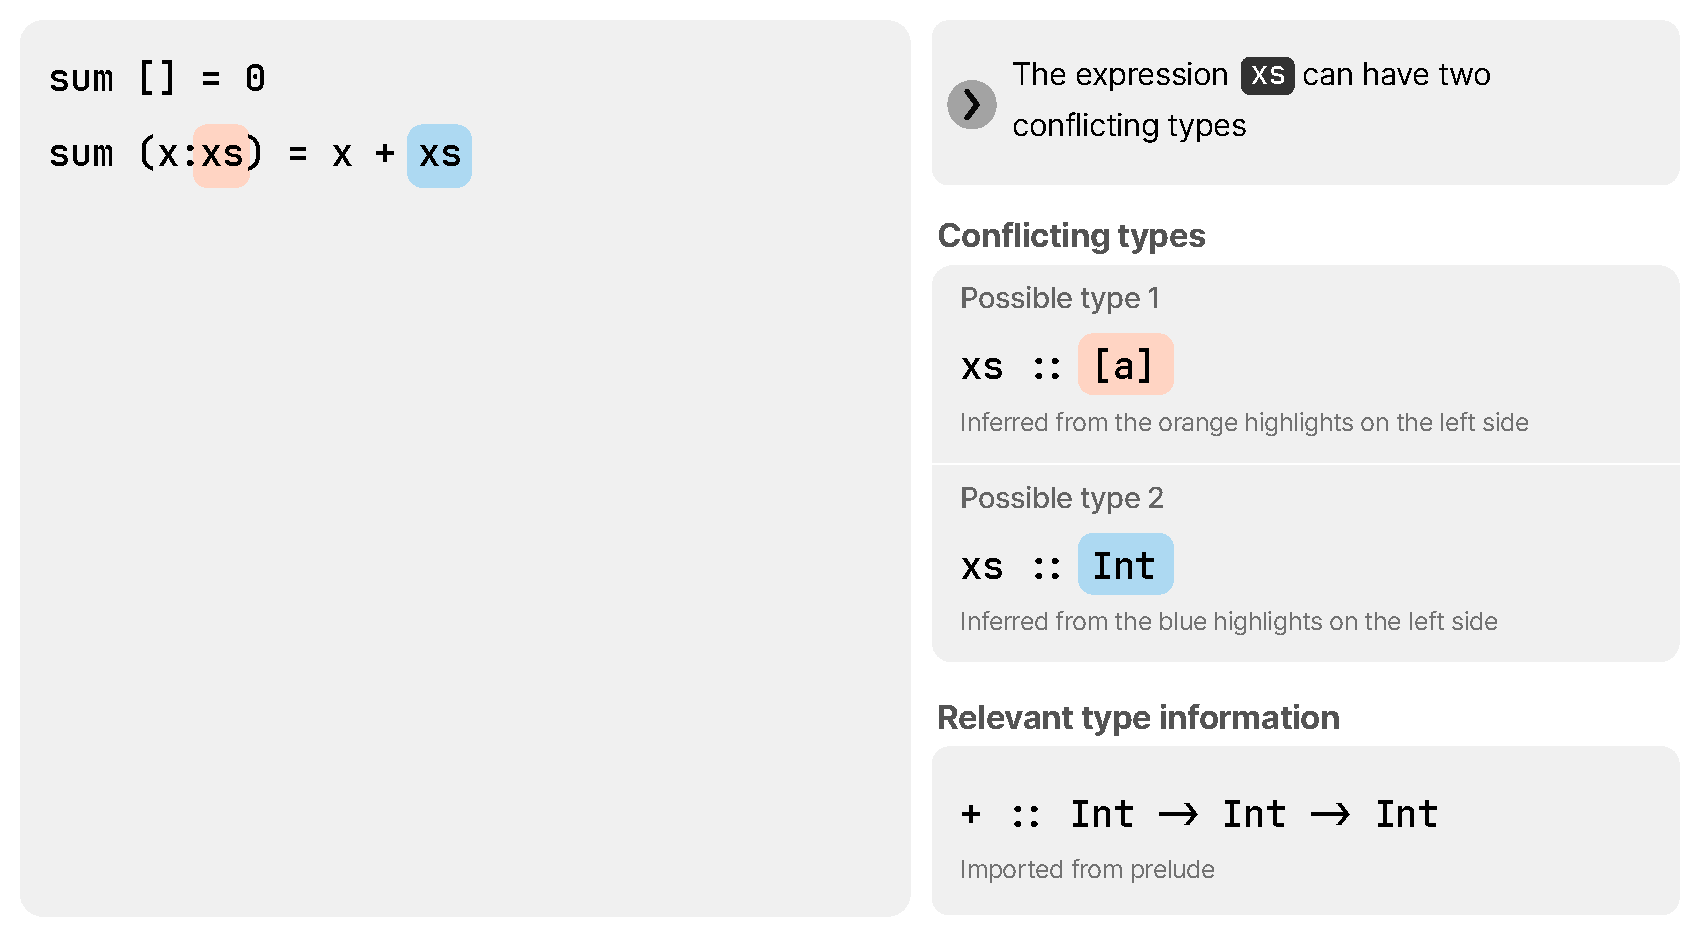
\includegraphics[width=\linewidth,trim=0mm 8mm 0mm 0mm]{images/basic-mode-1.pdf}
        \caption{
            Maxine's code to calculate the sum of a list of integers;
            \chameleon{} reports an error on the expression \texttt{xs}.
            }
            \label{fig:basic-mode-1}
\end{figure}

% \begin{figure}[h]
%         \centering
%         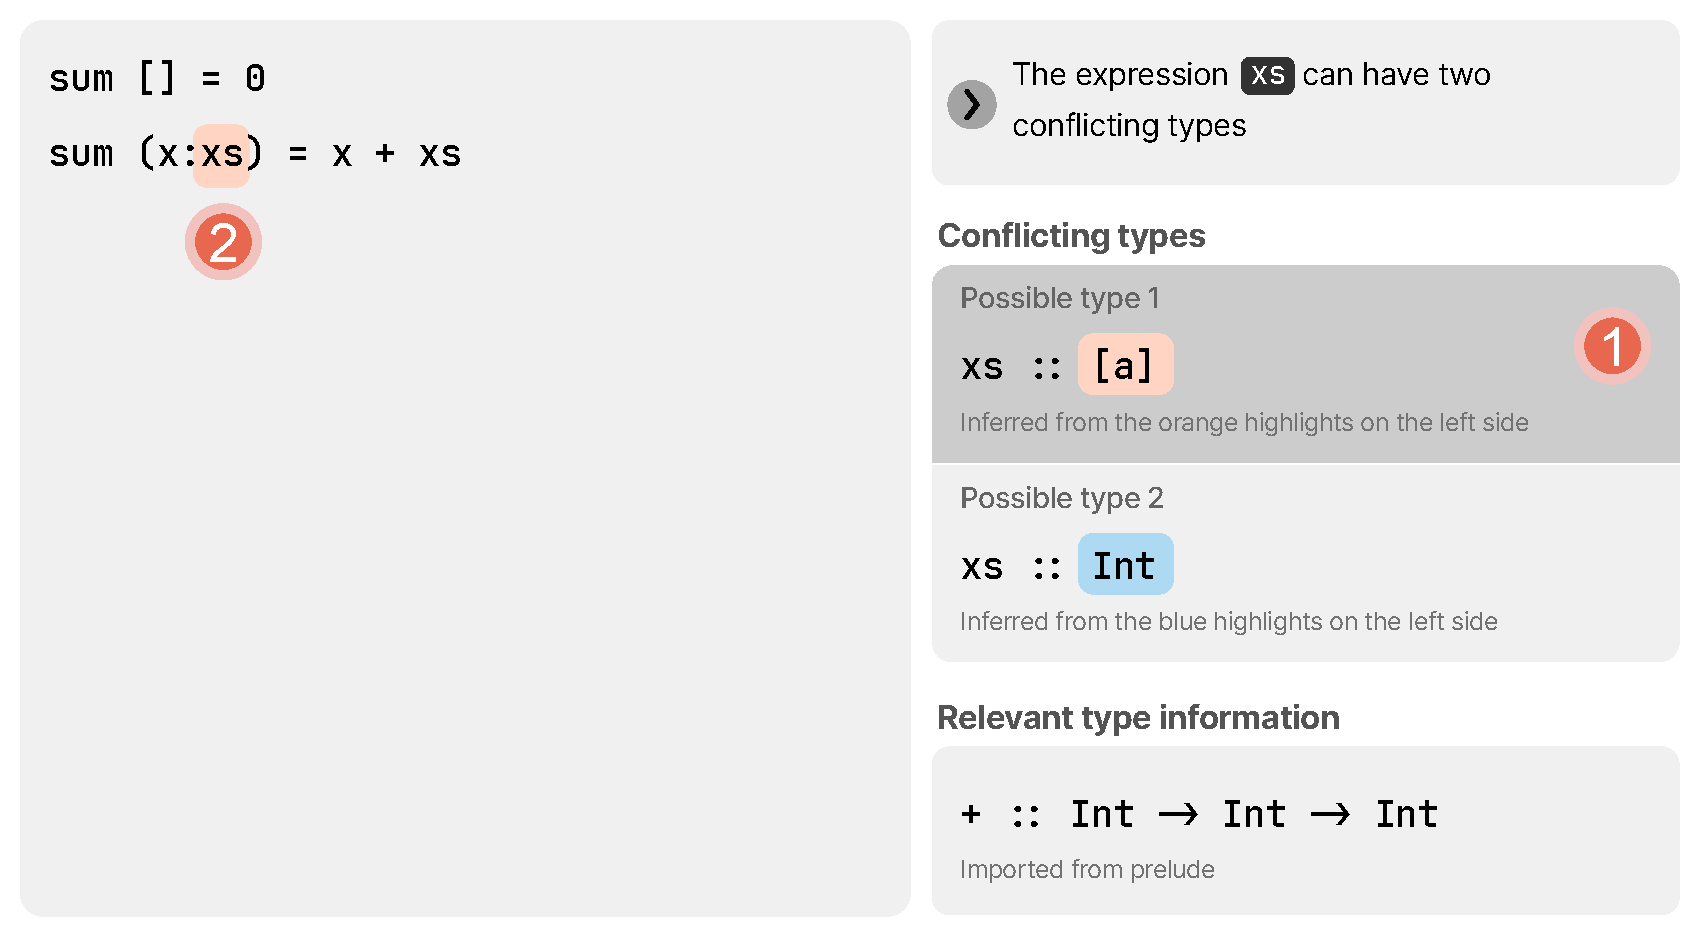
\includegraphics[width=\linewidth]{images/basic-mode-2.pdf}
%         \caption{
%        Hovering on possible type 1 will limit the highlights 
%        in the editor to only the ones (in orange) that support \texttt{x::[a]}.
%         }
%         \label{fig:basic-mode-2}
% \end{figure}

% \begin{figure}
%         \centering
%         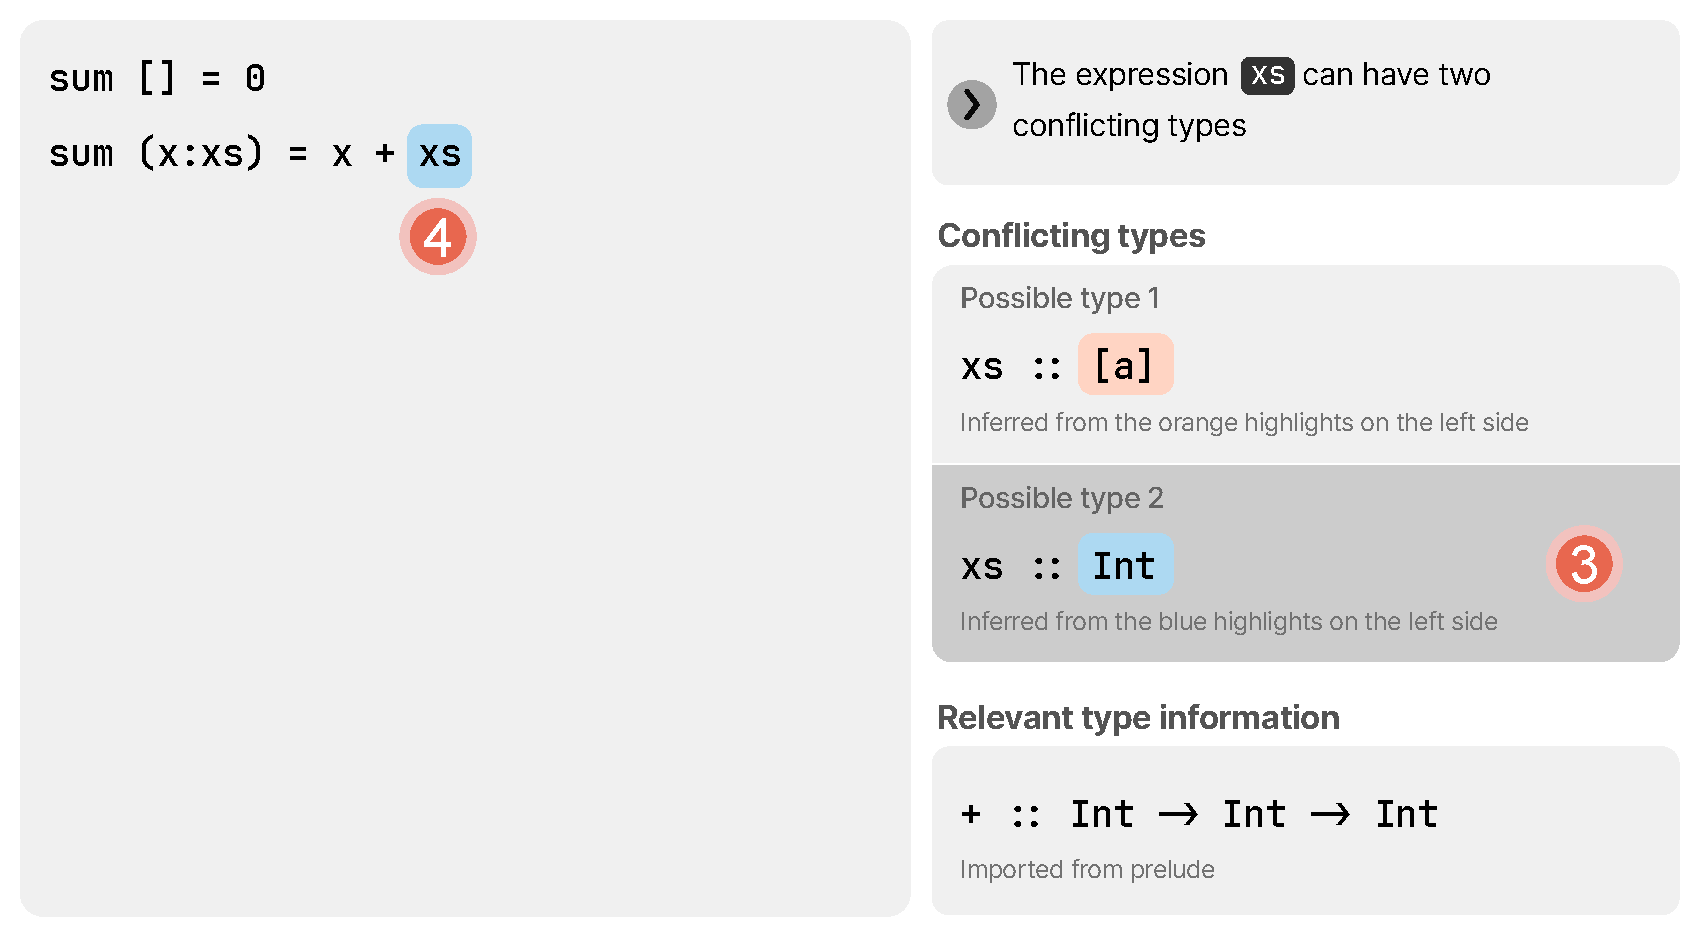
\includegraphics[width=\linewidth]{images/basic-mode-3.pdf}
%         \caption{
%             Hovering on possible type 2 (Fig. \ref{fig:basic-mode-2}-3) will limit the highlights 
%             in the editor to only the ones (in blue) that support \texttt{x::Int}.
%         }
%         \label{fig:basic-mode-3}
% \end{figure}





At this point, Maxine knows the possible type 1 aligns with her intention, and therefore, the error locations with blue highlights must be erroneous. After examining the program, it comes clear that Maxine forgets to apply the \texttt{sum} function recursively at the right-hand side of the addition. 


\subsection{Balanced mode} \label{sub:balanced}


Maxine writes additional code to add only even numbers in a list of integers, reusing the \texttt{sum} function she wrote earlier. After saving the file, \chameleon{} shows a type error in the expression \texttt{sum} (Fig.~\ref{fig:balance-mode-1}). However, this is not helpful because Maxine has just verified the implementation of \texttt{sum}. Switching to balanced mode, \chameleon{} shows two cards: \texttt{sum} and \texttt{evens}. 

\begin{figure}
        \centering
        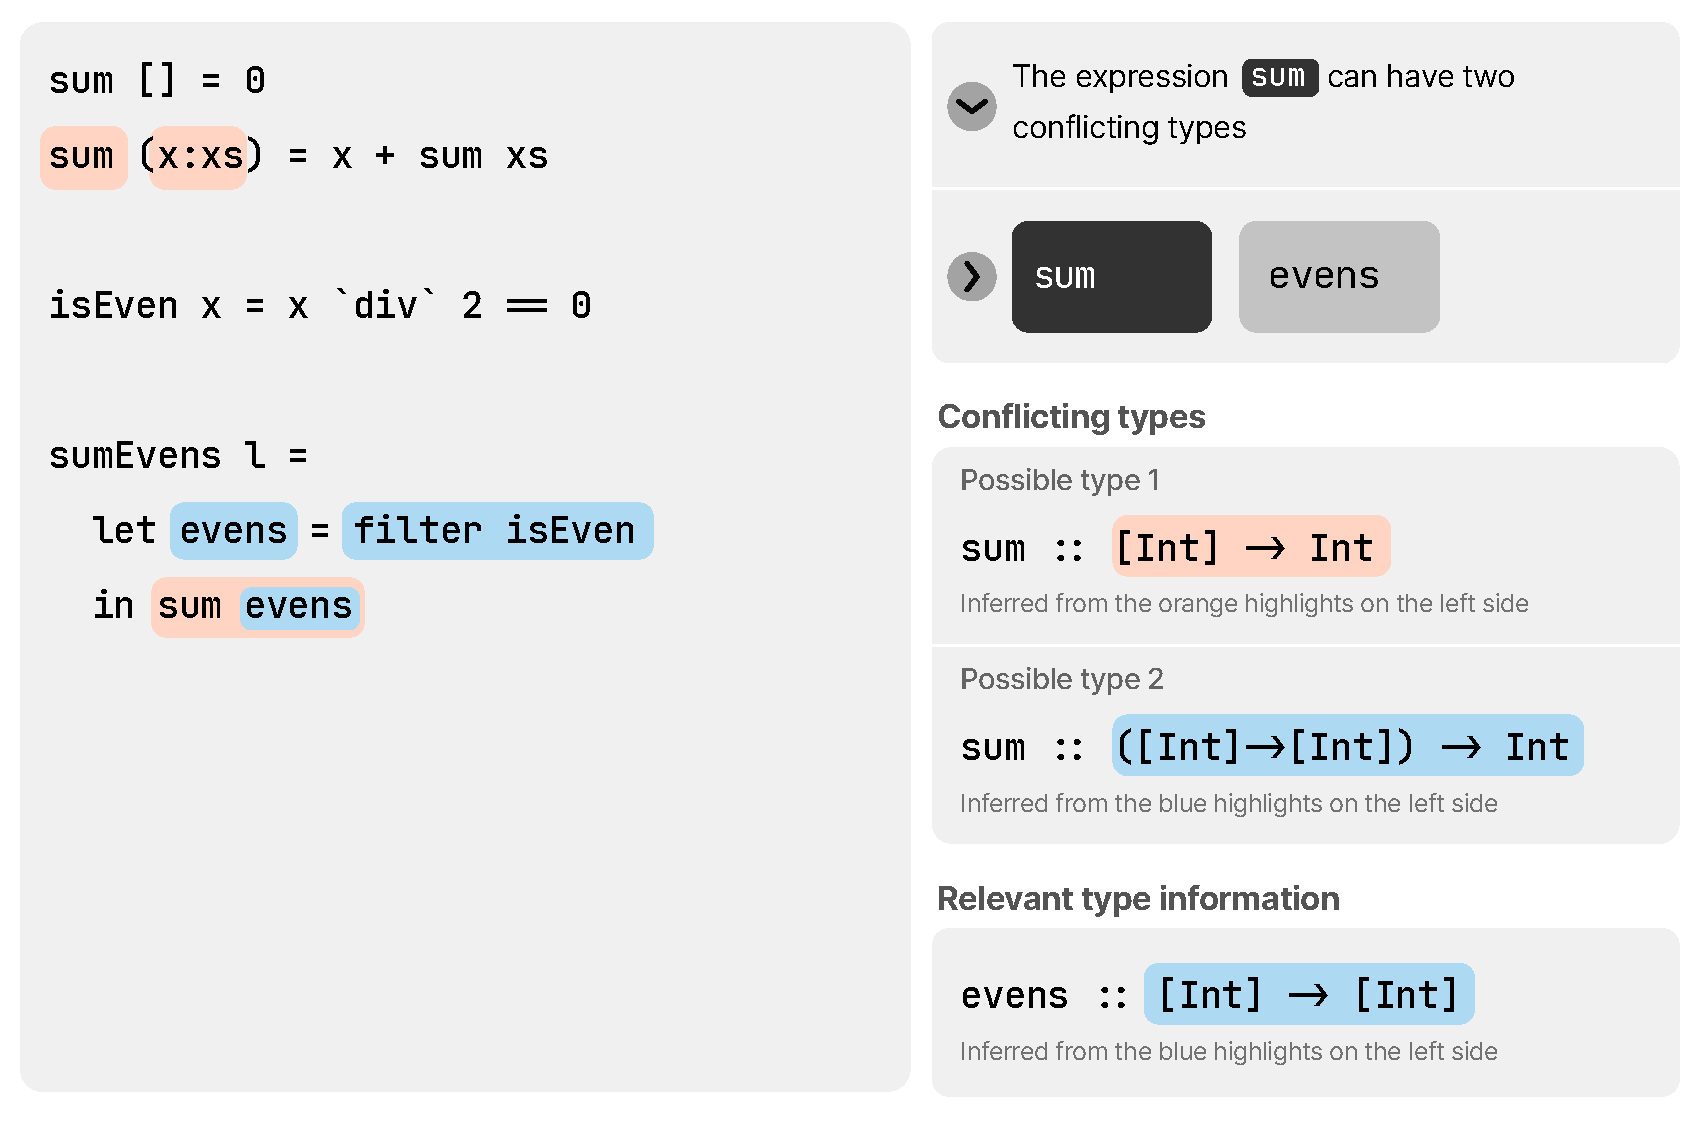
\includegraphics[width=\linewidth,trim=0mm 8mm 0mm 0mm]{images/balanced-mode-1.pdf}
        \caption{
            Maxine's code to calculate only the sum 
            of even numbers. \chameleon{} reports 
            an error with two candidate expressions.
        }
        \label{fig:balance-mode-1}
\end{figure}


\begin{figure}
   \centering
        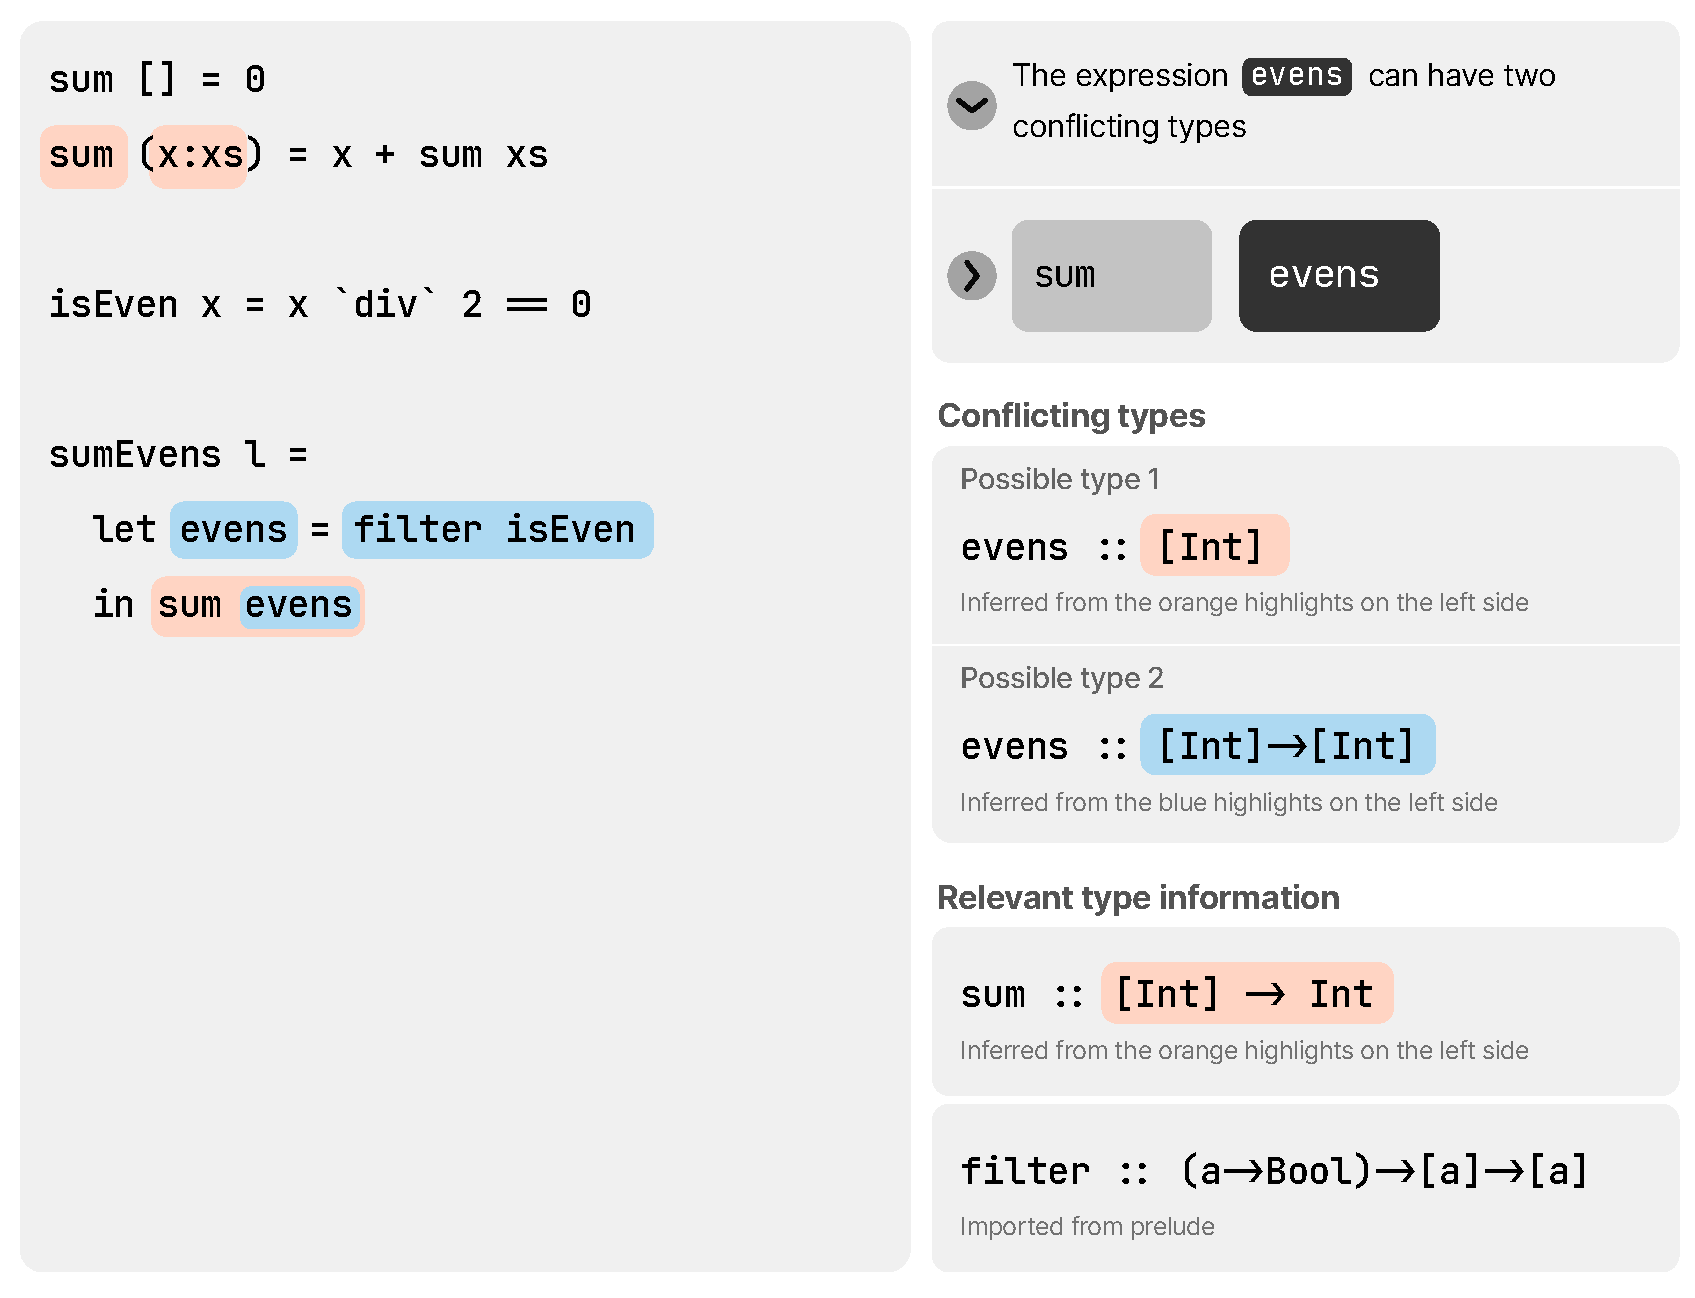
\includegraphics[width=\linewidth,trim=0mm 8mm 0mm 0mm]{images/balanced-mode-2.pdf}
        \caption{
            Clicking on the \texttt{evens} card (5) results in the changes in the
            conflicting types panel to show the possible types for \texttt{evens},
            and the changes highlight color to reflect the assumption that the
            definition of \texttt{evens} is the cause of the error.  
        }
        \label{fig:balance-mode-2}
\end{figure}

Maxine therefore clicks on the \texttt{evens} card and \chameleon{} reports two
possible types for the expression \texttt{[Int]} and \texttt{[Int] -> [Int]}
(Fig. \ref{fig:balance-mode-2}). Knowing the expression \texttt{evens} holds
a temporary list of even integers (hence it is of \texttt{[Int]} types), Maxine
concludes that the Possible type 2 is unintended. The locations with blue highlights must
contain the cause. It does not take long for Maxine to realize the list 
\texttt{l} is not supplied to the \texttt{filter} function.


\subsection{Advanced mode}  \label{sub:advanced}



\begin{figure}
        \centering
        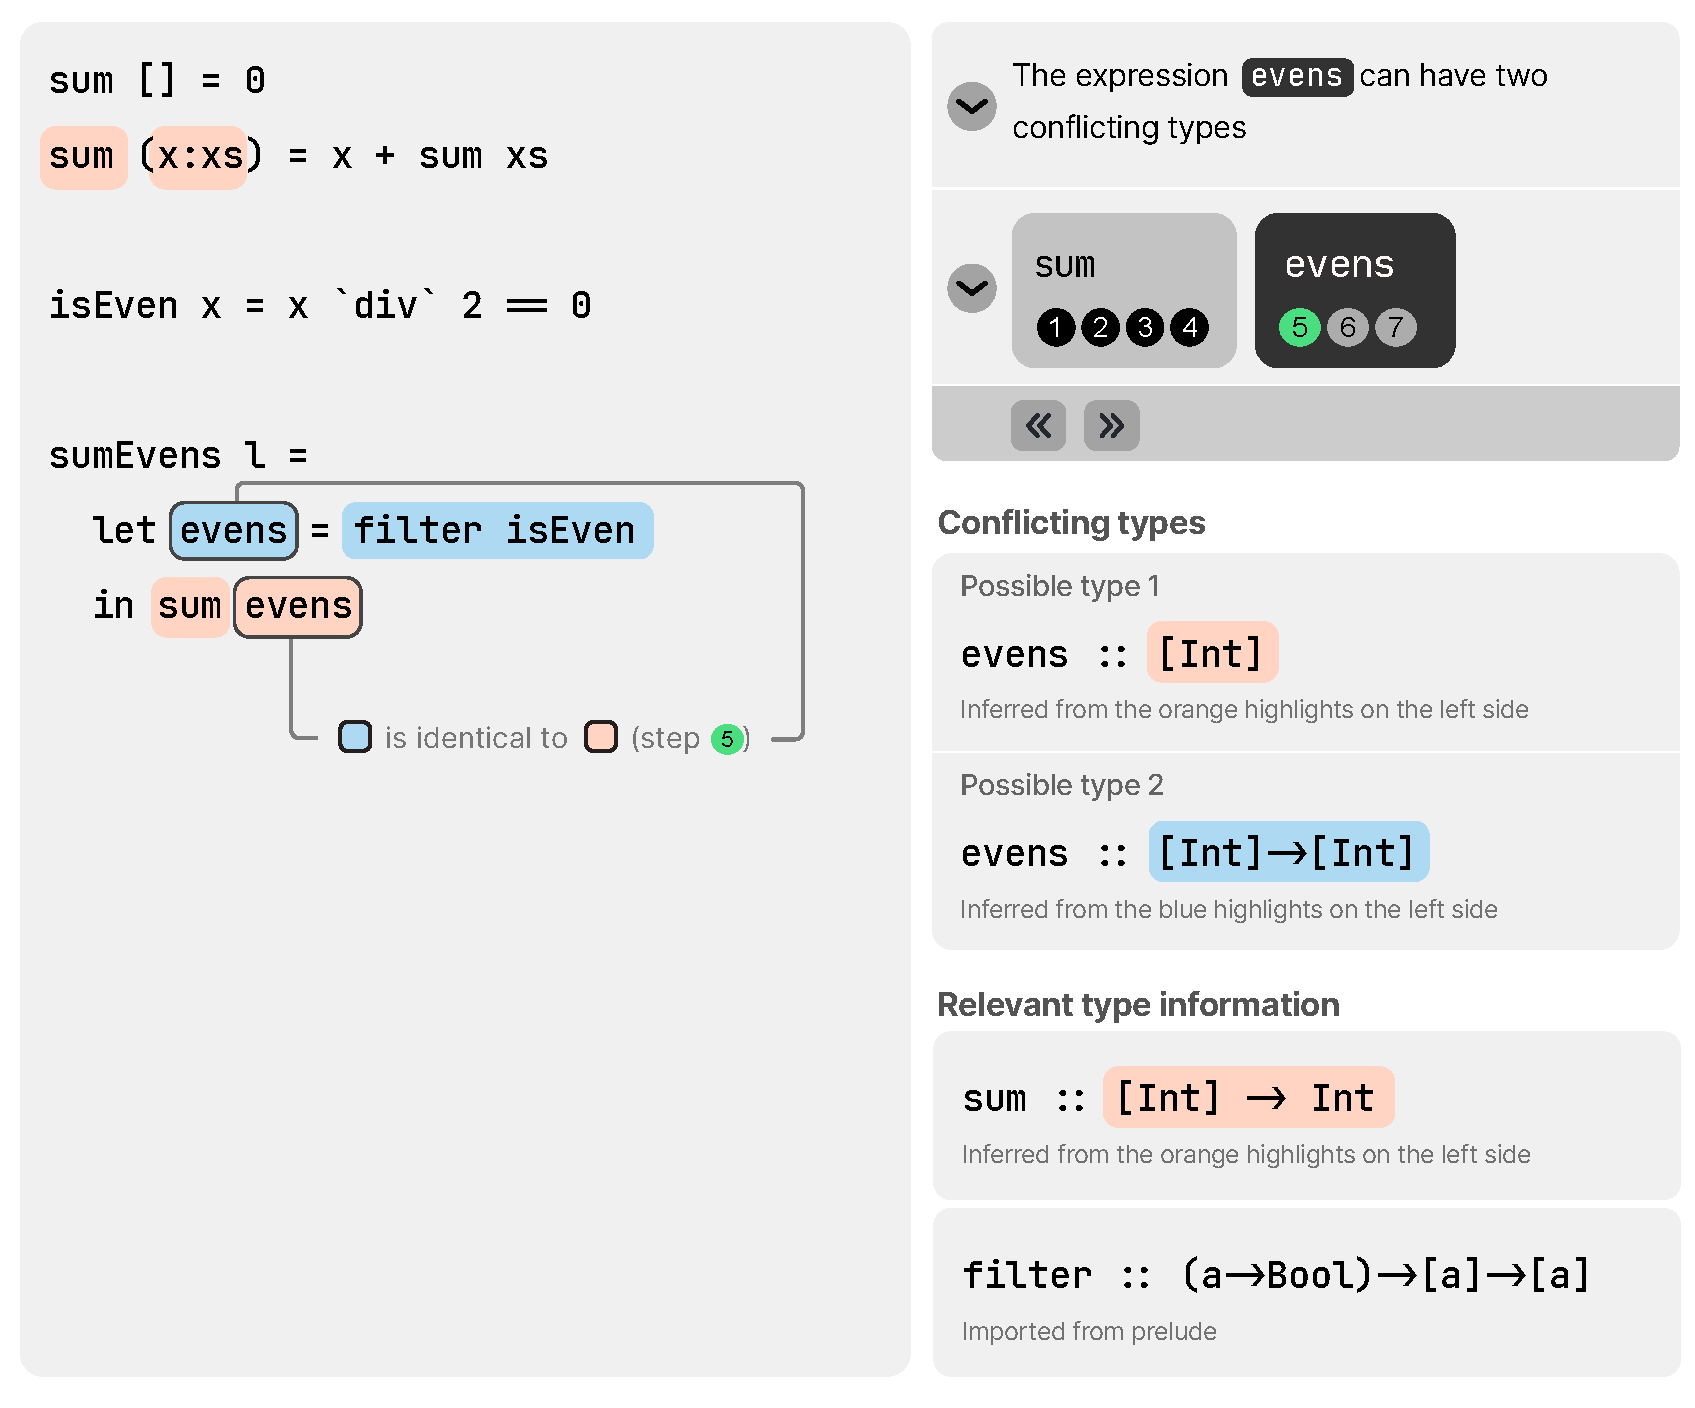
\includegraphics[width=\linewidth,trim=0mm 8mm 0mm 0mm]{images/advanced-mode-1.pdf}
        \caption{
            Maxine's code to calculate only the sum 
            of even numbers in advanced mode. 
            The current step is step 5, \chameleon{} 
            explains that the two appearances of expression 
            \texttt{evens} should have the same type.
        }
        \label{fig:advanced-mode-step5}
\end{figure}

\begin{figure}
        \centering
        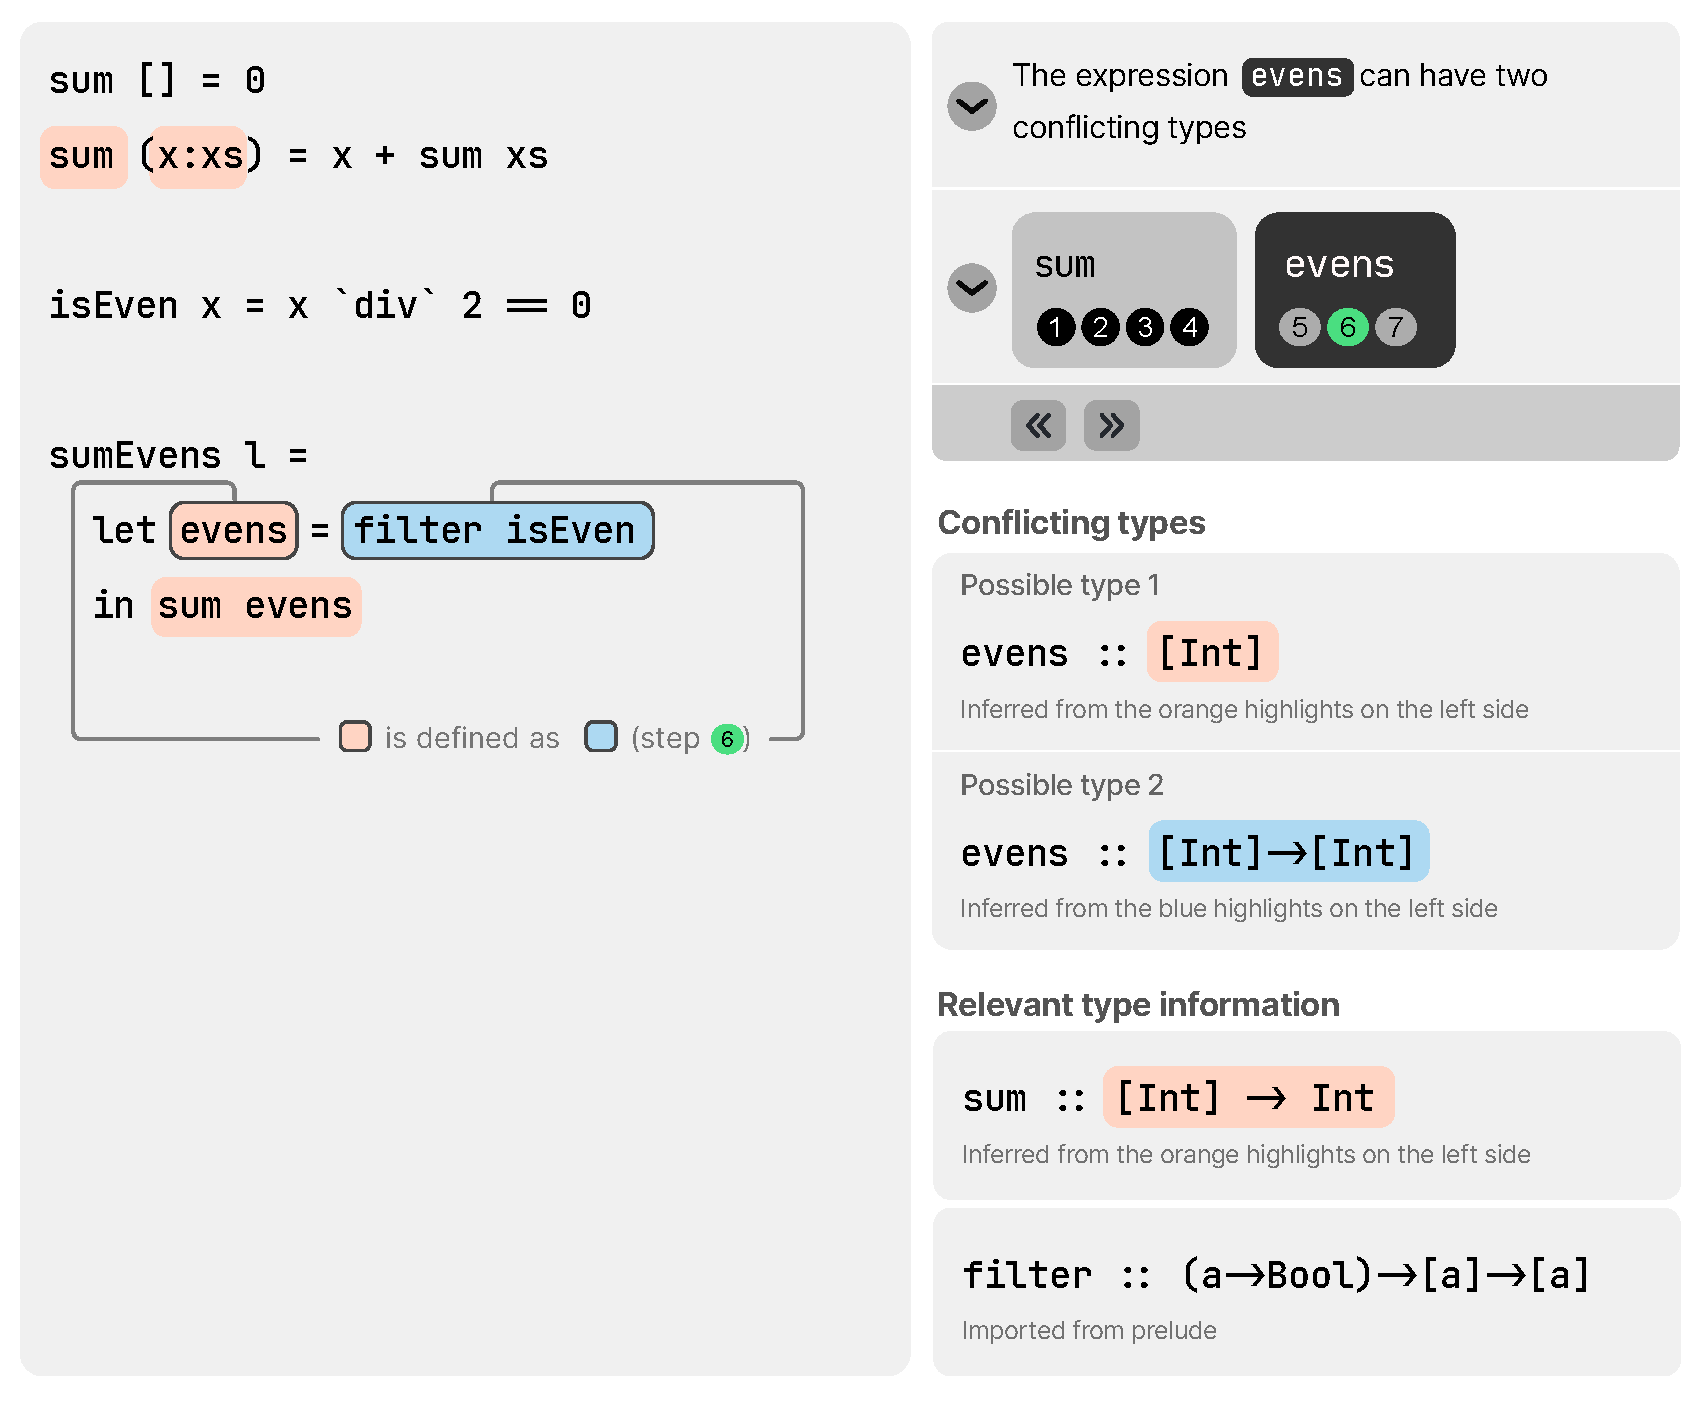
\includegraphics[width=\linewidth,trim=0mm 8mm 0mm 0mm]{images/advanced-mode-2.pdf}
        \caption{
            In step 6, \chameleon{} 
            explains that \texttt{evens} is defined as
            the expression \texttt{filter isEven}. The left-hand side
            and the right-hand side should have the same type.
        }
        \label{fig:advanced-mode-step6}
\end{figure}

\begin{figure}
        \centering
        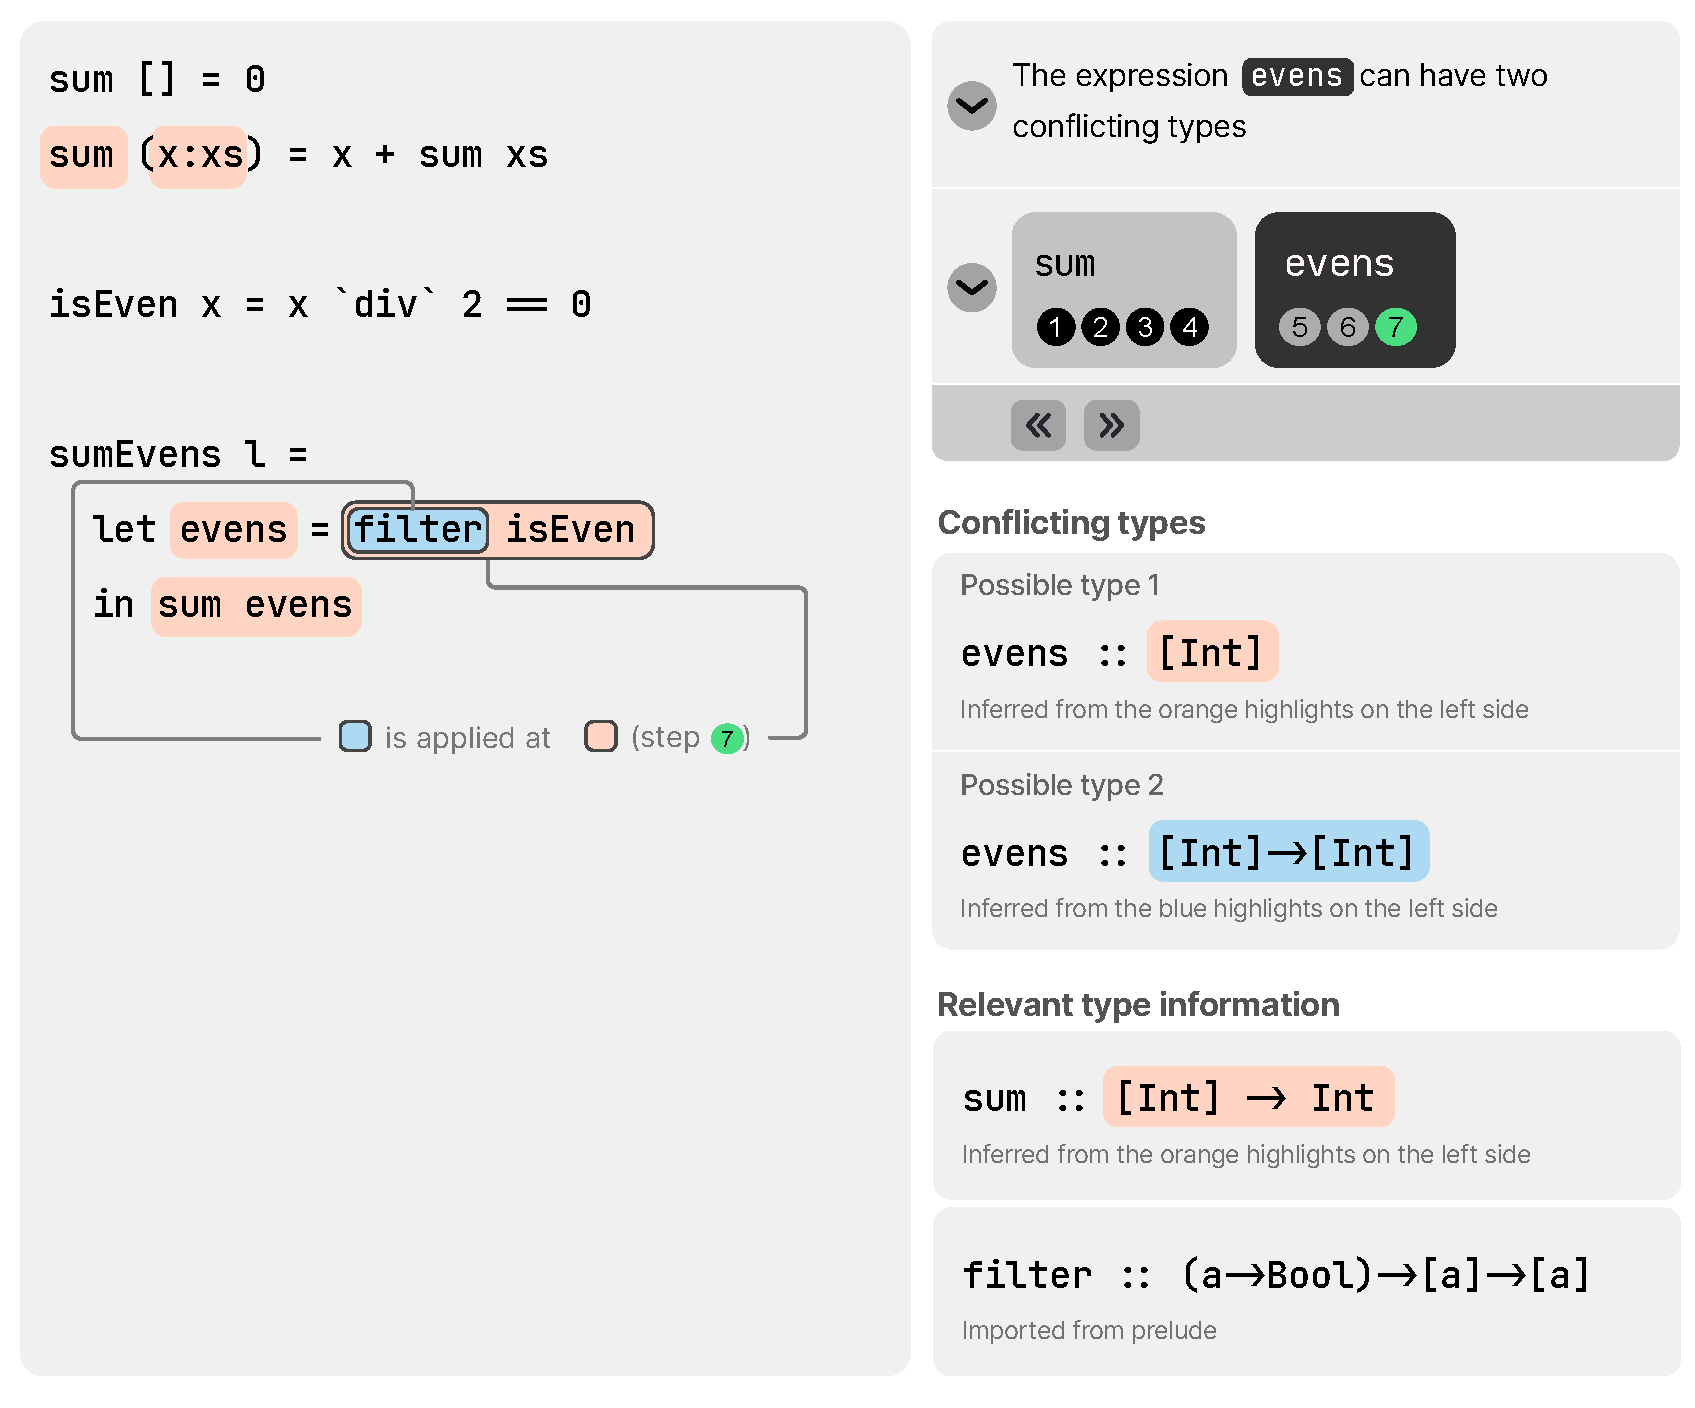
\includegraphics[width=\linewidth,trim=0mm 8mm 0mm 0mm]{images/advanced-mode-3.pdf}
        \caption{
            In step 7, \chameleon{} 
            explains that \texttt{filter} is applied to 
            the function \texttt{isEven}. Assisted by 
            the type of \texttt{filter} in the 
            Relevant Type Information panel on the bottom
            right, Maxine can find the type error that 
            \texttt{filter} expects two arguments but receives one.
        }
        \label{fig:advanced-mode-step7}
\end{figure}

% For the task shown in section \ref{sub:balanced}, if Maxine is not satisfied by
% the options provided by \chameleon{}, by switching to advanced
% mode, she has access to the debugging steps. 

To illustrate the deduction steps with the task shown in section \ref{sub:balanced},  first, Maxine clicks on step 5 (Fig. \ref{fig:advanced-mode-step5}) and verifies
that the two occurrences of \texttt{evens} are supposed to be identical, and the
second use means \texttt{evens} is a list of integers. Second, she
clicks on step 6 (Fig. \ref{fig:advanced-mode-step6}) and verifies that
\texttt{evens} should be the same type as the declaration on the right-hand
side. 


Lastly, Maxine clicks on step 7 (Fig. \ref{fig:advanced-mode-step7}), and
it shows that the \texttt{filter} function is applied to one argument
\texttt{isEven}. By consulting the relevant type information, Maxine identifies
that \texttt{filter} is expecting two arguments while only one is provided. 


\section{Evaluation}

We conducted three user studies, iteratively refining the \chameleon{} UI and evaluating several research questions as per Fig.~\ref{fig:timeline}. 
%The number of participants and their Haskell experience, as well as key research questions and conclusions, were shown in figure \ref{fig:timeline}. \todo{Explain was a user study of the tool with practitioners?}


\begin{figure}
    \centering
    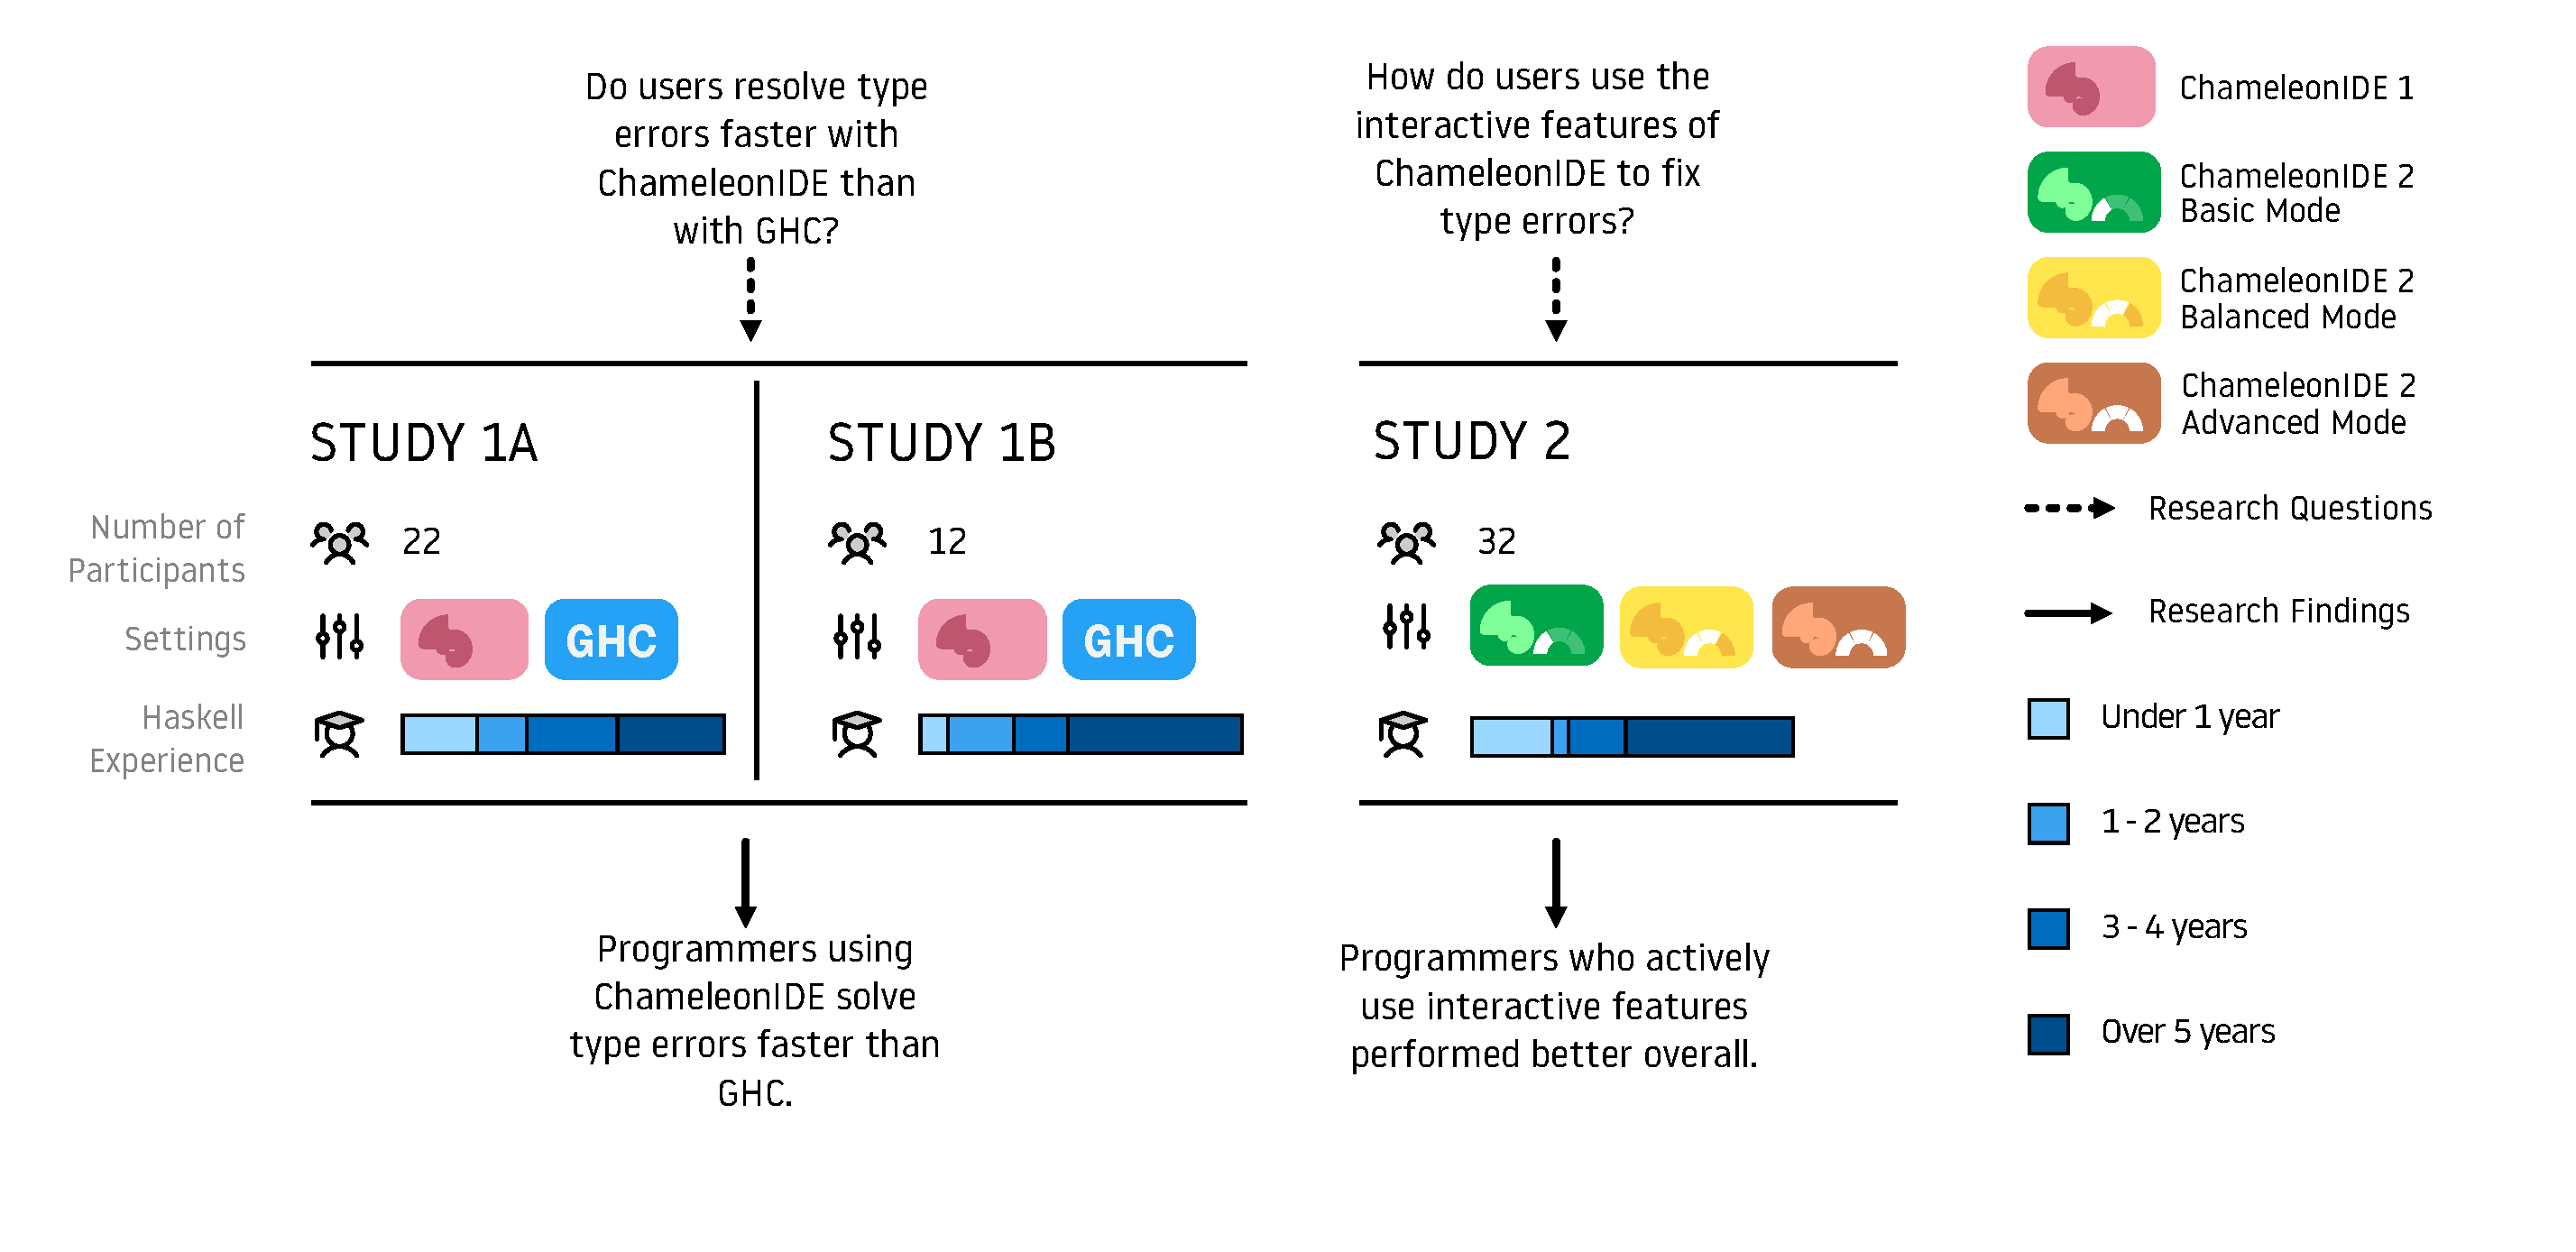
\includegraphics[width=\columnwidth,trim=30mm 35mm 35mm 5mm]{images/timeline.pdf}
    \caption{The timeline of \chameleon{}  evaluation.}
    \label{fig:timeline}
\end{figure}

\subsection{Experiment Design}
\subsubsection*{\textbf{Recruitment}}

Participants were recruited via the Reddit \textit{r/haskell} and \textit{r/programminglanguages} communities. 
%Recruiting from social media allowed us to access a more diverse demographic that better represent the true population of Haskell programmers. 
Participation is fully anonymized; detailed ethical implications of these experiments are reviewed and approved by the IRB of the authors' institution.


\subsubsection*{\textbf{Experiment setting}}
Experiments were conducted online and unsupervised. 
%Participants took the study online via a web browser and at the physical venue of their choosing. 
All user studies use a web-based debugging environment developed by the authors. 
%Conducting the studies online helped us avoid variation when performing tasks in unfamiliar places and using different setups. 


\subsubsection*{\textbf{Training and group assignment}}
After consent, participants received interactive training on the tool interface and interactive features. Participants were also shown a cheat sheet summarizing the key functionality of the interface, and had access to the cheat sheet at all times during the study. Participants were given 4 trial runs (2 for each setting) before the data collection started. 
All the studies used a within-subject design to evaluate the effectiveness of different tools or feature sets while counterbalancing the difference in programming proficiency between participants. In each study, participants were required to complete a series of programming tasks (8 for studies 1a and 1b, 9 for study 2). At each task, a participant receives a single Haskell file that contains one or more type errors. They were then asked to correct the code with the help of the given tool.


\subsubsection*{\textbf{Data Collection}}
Time is measured from the start of each task to the first time the program is successfully type-checked and also passes all the functional tests. Participants are able to skip a task if they are stuck. 
% The data is automatically recorded by the online debugging environment. To not introduce a barrier to completing the study, every task can be skipped if the participant made three failed attempts or is stuck for over 1 minute on the task.
After completing all tasks, participants are prompted to complete a debriefing survey. The survey questions include their Haskell experience and feedback on the tools.

We used a browser session recording tool~\cite{openreplay_openreplay_2022} to record the study sessions. This allows us to identify usability issues in the study and to recognize general patterns. 
%The reason we found this format inferior is that the recording technology does not provide a high enough sampling rate for us to be confidently used for rigorous analysis.
%One use of the session recording is for outlier trimming.  We identify participants who left the computer for an extended period of time. We first ran a statistical analysis to identify the long gap (2 standard deviations) between actions using program logs for each participant. Then, we manually checked with the session recording to verify there was actually no user input (mouse movement, scrolling). 

\subsection{\chameleon{} Human Studies}

\subsubsection{\textbf{\chameleon{} 1}}  
An earlier version of the UI than that depicted in Figs.~(2-13), it featured the type inference engine that recovers most concrete types after type errors occur and a minimal set of debugging features. Key features in \chameleon{} 1 include showing two (or more) alternative types, showing all possible error locations, dividing possible error locations into groups based on alternative types, and concrete type restoration. In short, \chameleon{} 1 is equivalent to \chameleon{} 2 set to basic mode. 

% \begin{figure}[h]
%     \centering
%     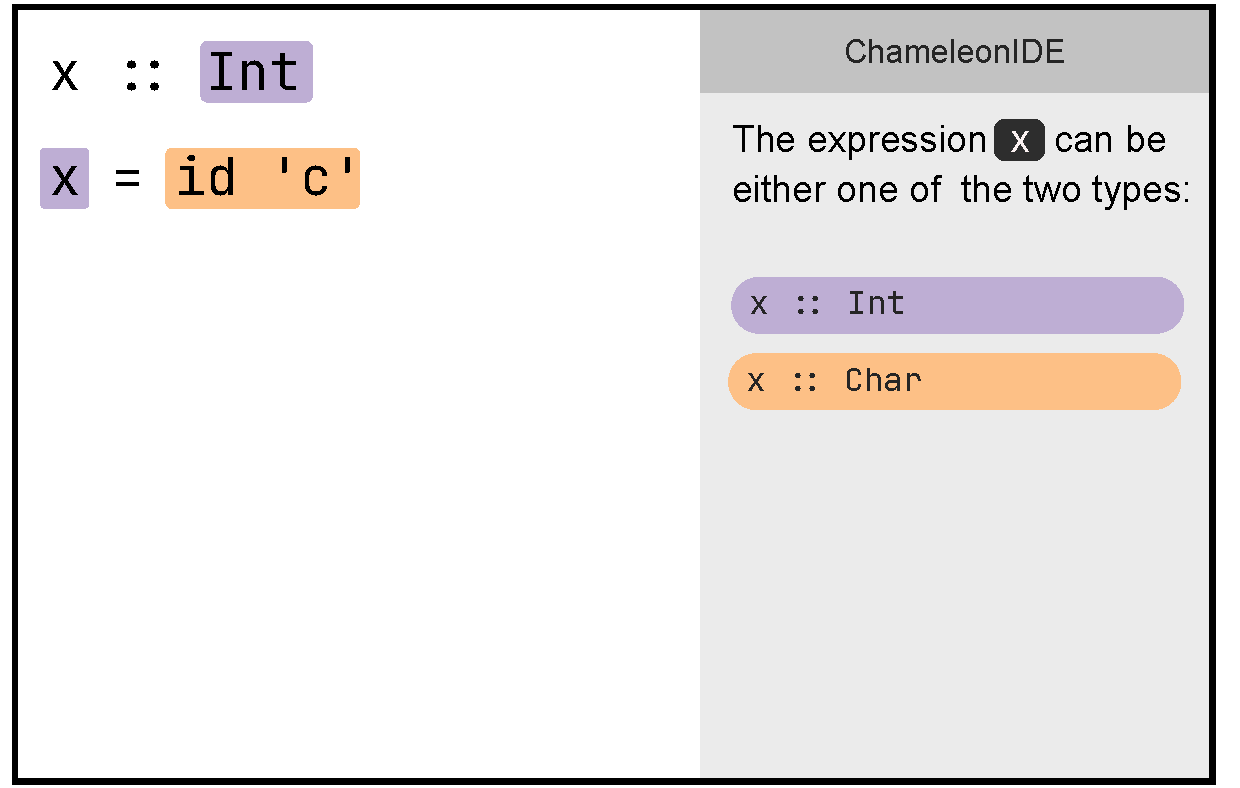
\includegraphics[width=\linewidth]{images/chameleon-v1.pdf}
%     \caption{
%         \chameleon{} 1
%         }
%     \label{fig:chameleon-v1}
% \end{figure}

Two  studies (1a \& 1b) were conducted to compare the effectiveness of solving type errors using \chameleon{} 1 and GHC compiler error messages. We choose GHC compiler error messages as the baseline because it is the canonical tool for working with type errors in Haskell.
%Although high-level tools like Haskell Language Server exist, they generally relay the GHC error messages verbatim. 
% The procedure of these studies is shown in figure \ref{fig:procedure-1}.


Eight tasks were given in both studies. In study 1a, the tasks were taken from the exercises of the Haskell programming class in the authors' institute. In the second study, the tasks are sourced from the top 20 Haskell topics on GitHub~\cite{github_github_2022}. The authors then manually added type errors into the program. In both studies, the type errors include simple mismatch, confusing syntax, missing instance, precedence and fixation, infinite types, and confusing list versus element. These categories follow the common type errors in Tirronen's study \cite{tirronen_understanding_2015}. 

Studies (1a \& 1b) address the research question:

\noindent\textbf{RQ1.} \textit{Do programmers solve type errors faster with \chameleon{} than GHC compiler error messages?}


% \begin{figure}[h]
%     \centering
%     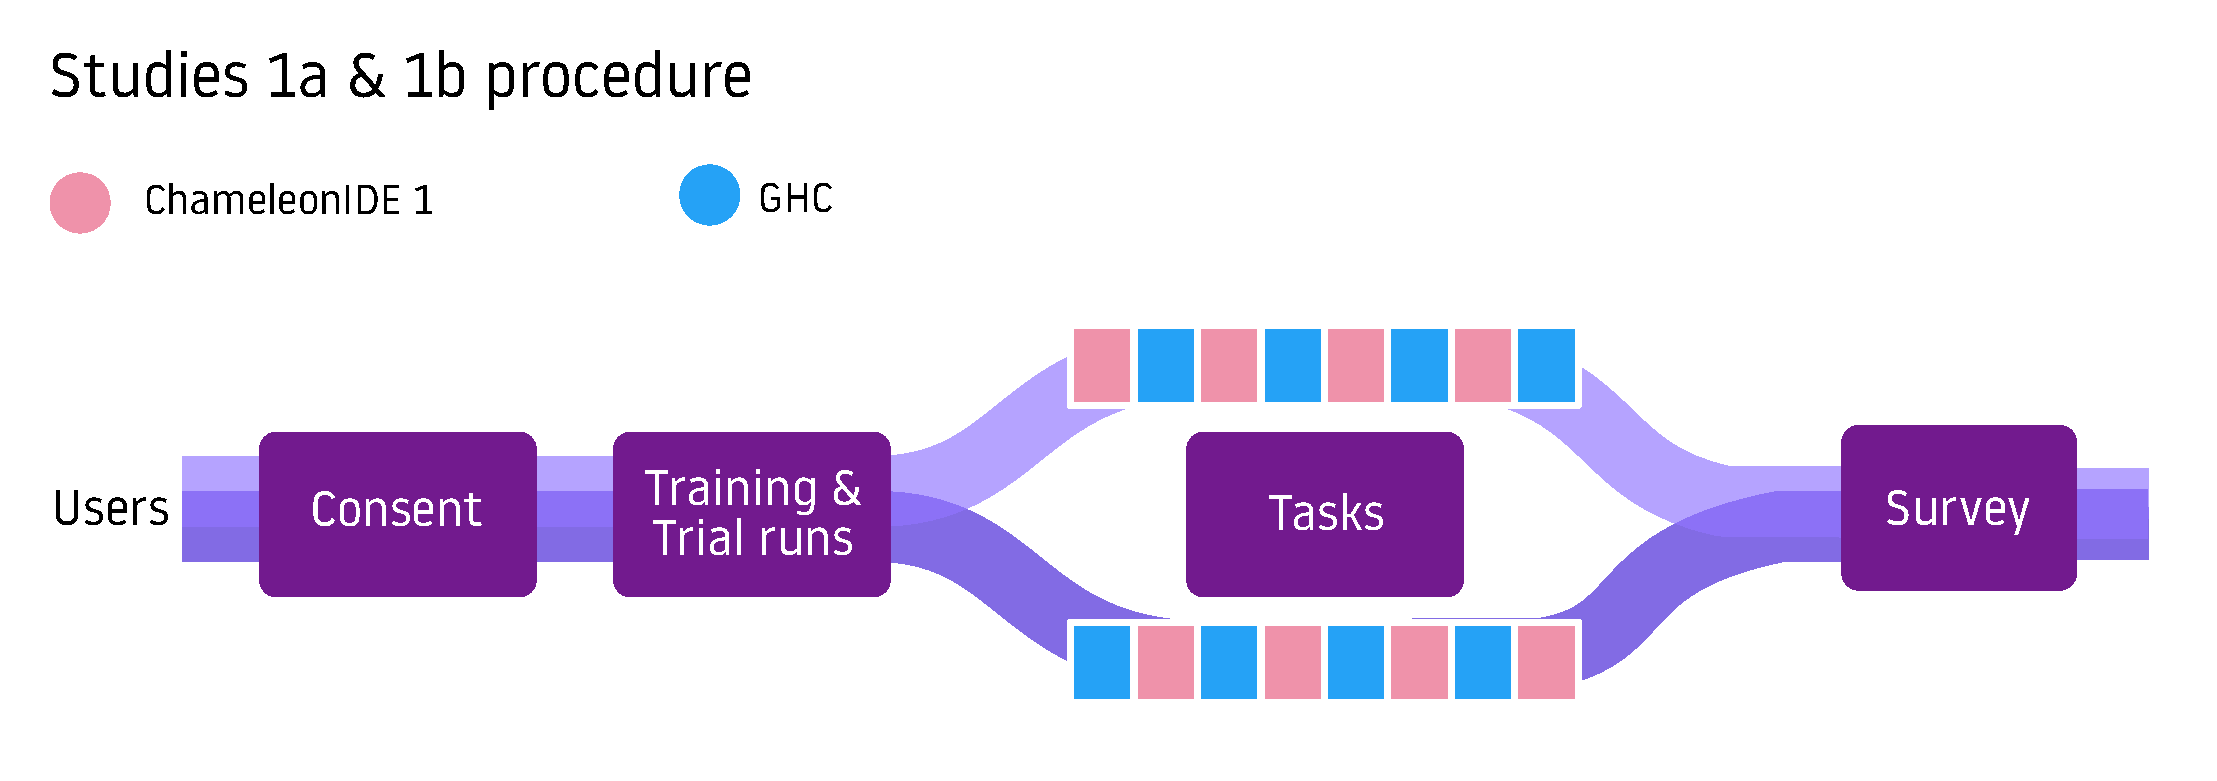
\includegraphics[width=\linewidth]{images/procedure-1.pdf}
%     \caption{\todo{Does this figure really help at all?}}
%     \label{fig:procedure-1}
% \end{figure}

% The study investigates the effectiveness of \chameleon{} compared to the GHC compiler error messages. We chose GHC compiler error messages as it is the canonical tool for debugging type errors in Haskell. Although high-level tools like Haskell Language Server exist, they relay the GHC error message verbatim for type errors. Participants are asked to complete 8 tasks. The tool participants used during each task alternated between \chameleon{} and GHC. Task programs were sourced from HaskellWiki \cite{haskellwiki}. The author manually added type errors. The errors cover a range of common Haskell type errors, including abstract data types, wrong arity, control expressions (if and case), infinite types, and tuples. The lines of code (LoC) range from 7 to 17 (mean = 11, median=10.5).


% In total 39 participants finished the study. Among them, 12 participants have over five years of Haskell experience, and 5 participants have three or four years of Haskell experience. And 8 participants have one or two years of experience, and 5 participants used Haskell for under a year. The rest left the question unanswered.

\begin{figure}
    \centering
    \includegraphics[width=0.8\linewidth,trim=15mm 12mm 15mm 35mm,clip]{images/user-study-1a.pdf}
    \caption{Study 1a task completion time (secs.) with 95\% confidence interval.}
    \label{fig:analysis-1a}
\end{figure}


\begin{figure}
    \centering
    \includegraphics[width=0.8\linewidth,trim=12mm 15mm 12mm 35mm,clip]{images/user-study-1b.pdf}
    \caption{Study 1b task completion time (secs.) with 95\% confidence interval.}
    \label{fig:analysis-1b}
\end{figure}

\subsubsection*{\textbf {Results}}

The data collected during study 1a, Fig.~\ref{fig:analysis-1a} does not show significant differences across Tasks 1-7. In hindsight, these tasks were trivial challenges for most users, and the individual differences among participants are generally more significant than the differences between treatments. However, one interesting observation is task 8, where the \chameleon{} group outperformed the GHC group. We attribute this significant difference to the difficulty of Task 8. The source file is longer and involves more language features (abstract data types and high-level functions). GHC struggles to produce a relevant error message for this type of error. 
From this result, we hypothesized that we might observe a more significant difference using tasks with lengthier and more realistic source code. 
This hypothesis is also supported by the most common feedback claiming that the tasks were too trivial to invite meaningful evaluation. One participant said, ``Looks nicer than GHC, but without trying it on something more complicated, I cannot conclude whether it would help me in practice." 

Therefore, in study 1b we introduced more difficult challenges and indeed observed that the \chameleon{} group was faster than the GHC group in almost all tasks (figure \ref{fig:analysis-1b}), barring task 1. A two-sample paired t-test was performed to compare the completion time between \chameleon{} and GHC groups. There was a significant difference between the two groups: $t(23) = -3.86, p = 0007$. For task 1, it is suspected that some participants spent more time exploring the interface of \chameleon{} due to its unfamiliarity. For all other tasks, from the video recordings, we saw many \chameleon{} users confidently skip reading unrelated chunks of code, while GHC users generally read through the whole program. In harder problems and messier code, we notice programmers start to report the benefits of \chameleon{}. ``It's most useful feature that I noticed was that it points out the locations of both conflicting uses; GHC often makes it difficult to figure out how it's coming to a conclusion about a type." reported one participant. ``I think \chameleon{}  does a much better job than GHC's error messages. I like that it shows the sources for the type judgments. This makes it quite easy to figure out how to rectify errors." reported another participant.

% \begin{itemize}
%     \item {It has a longer source file than other tasks (only shorter than task 6, but task
%     6 contains two independent type errors while task 8 is one connected task
%     error);}
%     \item {It is more complex than others (involves abstract data types and function application); and
%     }
%     \item {
%         GHC struggles to produce a relevant error message for this type of error.
%     }
%   \end{itemize}


  

% \begin{figure}[H]
%     \centering
%     \Description{A screenshot from user study 1}
%     \includegraphics[width=\textwidth]{round1-screenshot.pdf}
%     \caption{
% One participant working with \chameleon{}  managed to identify the most probable location of the error (the application of `fromMaybe'` on line 11) by hovering over the two alternative types. The participant then quickly realized that the first argument `0` (highlighted in orange) is inconsistent with the definition where it is case matched to a `Nothing` value (highlighted in purple). After two retries with short hesitation the participant found the correct fix (by reversing the order of `0` and `n`).
%     }
%     \label{fig:r1-task8}
% \end{figure}


% \begin{figure}[htb]
%     \centering
%     \Description{A screenshot from user study 1}
%     \includegraphics[width=\textwidth]{round1-screenshot-ghc.pdf}
%     \caption{
%         In task 8, participants using GHC took longer pauses at this task before committing to further investigation, either carefully reading the whole text or figuring out the meaning of the error message. The GHC error message is unfortunately unhelpful for this task.
%     }
%     \label{fig:task8-ghc}
% \end{figure}




\subsubsection{\textbf{\chameleon{} 2}}  \label{sub:us4}
Based on observations of Study 1 we introduced several new features to \chameleon{}, eventually resulting in the UI depicted in Figs.~(2-13). Interactive features were available in this iteration, such as deduction steps, candidate expressions, and mode switching. A few other user interfaces \cite{anonymous_interactive_2021} were designed and prototyped between the development of \chameleon{} 1 and \chameleon{} 2. Study 2 addresses the research question: 

\noindent\textbf{RQ2:} \textit{How do programmers use the interactive features in \chameleon{} 2?}. 

More specifically:
\begin{itemize}
    \item \textbf{RQ2.1} How do programmers use the advanced features provided by \chameleon{} 2?
    \item \textbf{RQ2.2} Do programmers prefer switching modes during debugging type errors?
    \item  \textbf{RQ2.3} What are programmers' preferences among the three modes provided by \chameleon{} 2?


\end{itemize}

During each run, the initial mode of each task alternated through the three different modes and repeated three cycles in nine tasks. The order of the three modes in each cycle is counterbalanced among all participants. However, participants can switch to other modes at any time. 



% \begin{figure}[h]
%     \centering
%     \includegraphics[width=\linewidth]{images/procedure-2.pdf}
%     \caption{\todo{Does this figure really help at all?}}
%     \label{fig:procedure-2}
% \end{figure}

\subsubsection*{\textbf{Results}} 

Study 2 is more exploratory in methodology than Study 1. We encouraged programmers  to discover their way of using the tool. In post hoc analysis of the collected log data, we were able to extrapolate some interesting patterns of how the tool was used. 


\textbf{RQ2.1}. The most striking feature of the data is that users tend to vary wildly in their use of the tool. Some users used the features extensively, while others completed the tasks without actively exploring the given information. Based on this discrepancy, we divided the users into three groups in table~\ref{tab:interaction-level}.
\begin{table}
    \centering
\begin{scriptsize}
\begin{small}
\noindent\begin{tabularx}{\linewidth}{ 
  | >{\hsize=.26\hsize}X 
  | >{\hsize=.74\hsize \raggedright\arraybackslash}X  | }
    \hline
        Interaction level & Description \\ \hline
        \textit{Minimal}  & Users completed the tasks by making changes in source code, type checking, and reading error messages. \\ \hline
        \textit{Low}  & Users only actively used universal features in all modes, for example, hovering on "Possible type 1" and "Possible type 2" to narrow down error space. \\ \hline
        \textit{High}  & Users did everything from the low interaction group but used features specific to the Balanced mode and the Advanced mode, such as activating steps and expression cards. \\ \hline
\end{tabularx}
\end{small}
\end{scriptsize}
    \caption{Levels of programmer interaction and their description}
    \label {tab:interaction-level}
\end{table}

As shown in  Fig.~\ref{fig:r4-analysis}, the time to complete each task roughly relates to the interaction level of participants. Participants with higher interaction levels generally performed better, and the lowest interaction level was worse. Tukey’s HSD Test for multiple comparisons found that the completion time was significantly different between the minimal interaction group and the high interaction group ($p \le 0.001$, 95\% C.I. = [18.26, 31.41]), and between the minimal interaction group and the low interaction group ($p \le 0.001$, 95\% C.I. = [11.96, 26.67]). The results from three tasks stand out from the general trend: in Tasks 4 and 6, higher interaction users performed worse, and in task 9, the general trend is exaggerated. As with Study 1a and 1b, this difference is likely related to task difficulty. Tasks 4 and 6 are shorter than other tasks. The ideal fixes for these two tasks are placed relatively early in the source code (both in the first two lines of the source code). Users simply reading top to bottom could quickly identify the error without needing to skip unrelated sections of code using the information provided by \chameleon{}. This reduced the apparent benefit of \chameleon{} in these tasks. On the other hand, task 9 is the lengthiest task of all. It also involves deeply nested type definitions that are harder to follow in mind.

\begin{figure}
    \centering
    \includegraphics[width=\linewidth,trim=0mm 15mm 0mm 50mm,clip]{images/user-study-2.pdf}
    \caption{Study 2 task completion time (secs.) with 95\% confidence intervals.}
    \label{fig:r4-analysis}
\end{figure}


% \begin{figure}[h]
%     \centering
%     \includegraphics[width=\linewidth]{images/r4-task9.png}
%     \caption{
% High interaction users were able to locate the exact line for a potential fix after navigating to deduction step 6 or 7, which directly revealed the true cause of the type error. After this, 12 out of 15 high interaction users provided the most ideal fix in the first try. Low interaction group  takes longer time to examine the problem, provided wrong fixes in the initial trials. One participant fixed a minor run-time issue (a problematic pattern matching of `[attributes]` on line 18) however failed to identify the culprit of the type error. This location is not pinpointed by \chameleon{} and therefore it is understandable that programmers who used the deduction steps would be able to ignore this part of the source code.
%     }
%     \label{fig:r4-task9}
% \end{figure}


Another observation is when using the mode switching feature of \chameleon{}, we show this by presenting the starting mode and finishing mode of each task and each participant in a correlation matrix (Fig. \ref{fig:r4-mode-switching}). This observation suggests two characteristics of using multi-mode debugging tools. First, to answer \textbf{RQ2.2} programmers are roughly splitted in this matter: 53\% changing modes vs. 47\% staying in the same mode. Second, to answer \textbf{RQ2.3} when changing modes, programmers generally switch to the more informative modes instead of the more concise ones.
\begin{figure}
    \centering
    \includegraphics[width=0.7\linewidth,trim=0mm 5mm 0mm 5mm,clip]{images/mode-switching.pdf}
    \caption{Study 2 mode switches by starting mode.  Users overwhelmingly switched to the more sophisticated interface mode.
        % The rows represent the finishing mode, columns starting modes.
    }
    \label{fig:r4-mode-switching}
\end{figure}


\subsection{Limitations}

One threat to the validity of the evaluation is the number of participants. Although for each study we received hundreds of online participants, the studies suffered from a high abandonment rate (especially study 1b). This was expected: the programming challenges are difficult, and our volunteer participants are unremunerated. 
Because we recruited participants online and anonymized all the participants, it is possible for participants of a previous study to enter a later one. This creates variation in familiarity. We offset this by using new code challenges in every study and conducting trial runs before data collection to bring new participants up to speed.
Conducting studies remotely and unsupervised left us no means to intervene when users encounter usability issues. To mitigate this, we conducted cognitive walkthroughs and sandbox pilots before running each study.

Future evaluation would benefit from using more realistic tasks. The tasks in our human studies do not get as complex as professional Haskell programmers may face in a typical production codebase. It would be interesting to see how \chameleon{} is used against type errors that span multiple files and packages and include more confusing abstractions, like Monads, Monad transformers, and Lenses.

\section{Discussion}

% \todo{Suggest try and strucuture this a bit more e.g. each para bold the key lesson @ start of para. Can you group into implications for research/implications for practice to make more actionable??}

This paper presents the interactive type debugging tool \chameleon{} and charts the evolution of its design across several iterations in response to user evaluation and feedback, as well as examines   the effectiveness of the general approach compared to traditional static type error messages. We found that programmers using \chameleon{} are able to debug errors faster than using traditional text-based error messages. This effect is shown more clearly when the task is not trivial. We found that programmers who actively use \chameleon{}'s interactive features are more efficient in fixing type errors than passively reading the type error output. In this section, we will discuss a few interpretations of the results.


\subsection{Effect on Reading Source Code}
From the results of Study 1a, we observed that the choice of debugging tool had little effect on how fast programmers solve simple type errors. Conversely, when facing more realistic problems (longer source code, error locations more scattered) in study 1b, programmers are more effective using \chameleon{}. One explanation is that \chameleon{} reduces the amount of reading time by taking programmers more directly to the problem. Earlier studies \cite{Jbara2015-gr, Peitek2020-nb} showed that reading source code is generally the initial step of solving programming problems and is done in several passes. Although traditional compiler error message tools initially show fewer locations, these may be incomplete, meaning that programmers have to expand the reading span without clear guidance. In contrast, \chameleon{} shows more error locations initially. However, the completeness of error locations assures programmers which part of the source code can be safely skipped.

\subsection{Forming Debugging Plans}
From the results of Study 2, we found that programmers who use the interactive tool fix type errors faster than the ones who passively read the error output. This effect is stronger in harder tasks. We speculate that one factor of this result is that  \chameleon{} helps to develop debugging plans. We observed that when working with \chameleon{}, programmers form different debugging plans to attack the problem. Among the \textit{high} interactivity participants in user study 2, some programmers cycle through deduction steps as a guide to reading source code; some navigate to both ends of the deduction chain where types are normally grounded and concrete. In contrast, \textit{minimal} interactive participants generally form similar plans, including carefully reading the program text and manually annotating expressions based on their understanding of the program.


\subsection{Externalize Intermediate Typing Information}
We speculate another factor of the effectiveness of \chameleon{} interactive debugging tools is that they help programmers effectively chunk intermediate information. With the program shown in Fig.~\ref{fig:listing2}, \chameleon{} offers two candidate expressions: \texttt{f} can be typed as \texttt{Int -> Bool} or \texttt{Char -> Bool}; \texttt{z} can be typed as \texttt{Int} or \texttt{Char}. Although  these two statements are equivalent in theory, programmers are often required to compute the latter from the former or vice versa. And this computation may carry out multiple layers. Programmers have to remember all the intermediate types and their reasoning throughout such mental gymnastics. Assisted by candidate expression cards and deduction steps, this intermediate information is externalized on screen and can be retrieved anytime. A recent study on working memory \cite{Crichton2021-ru} suggested this approach may provide a positive effect in helping programmers manage cognitive load and free up working-memory space for high-level thinking.

% \subsection{Implication for future studies}
% Our study aims to contribute to the wider understanding of program comprehension in the context of advanced type systems. One promising research area to extend our results is to apply the design of \chameleon{} to other languages with high demand for explainability\cite{ferdowsi_usability_2023}.

% Colorization and overlay widgets are used to visualize relations and orders that may not conform to the source code structures. These techniques fit well to types because the introduction and elimination of typing constraints tend to be scattered throughout the program. A interesting question is whether these techniques can also be applied to other program properties, such as memory allocation and freeing, as well as message dispatching and consumption, which also exhibit similar patterns.

% Finally, we employed MUS (minimal unsatisfiable subset) for fault localization and types recovery, but we are also curious about the possibility of further analysis based on MUS to power advanced debugging systems, such as efficient and accurate type error repair by combining our results with mutation testing or solution searching based on machine learning.

\begin{figure}[ht]
    \centering
    \includegraphics[width=0.4\linewidth]{images/Listing2.pdf}
    \caption{\chameleon{} reports an error in the expressions \texttt{f} and \texttt{z}}
    \label{fig:listing2}
\end{figure}

% \begin{listing}
% \begin{minted}[bgcolor=bg,linenos]{haskell}
% f z     
%     | z == 3 = False
%     | z == '4' = True
% \end{minted}
% \vspace*{-9mm}
% \caption{\chameleon{} reports an error in the expressions \texttt{f} and \texttt{z}}
% \label{listing:2}
% \end{listing}
% Implication for research
% In our studies, \chameleon{} shows a few different designs for type error visualization and interaction. However, we are far from exhausting the search space. One challenge we notice in the current design is that programmers have to shift their focus between the editor on the left and the \chameleon{} debugging interface on the right. Using the hover popup window in most mainstream IDEs may reduce the context switching during debugging.

% Integration with existing tools
% The current implementation of \chameleon{} requires non-trivial adaptation for editors such as VS Code and IntelliJ due to the overlay explanation layer. This type of error visualization is non-standard in mainstream editors. However, there may exist alternative representations of \chameleon{} error reporting using only the features available in major editors and IDEs. It is especially beneficial to represent \chameleon{} errors using a universal debugging middle layer such as language server protocol (LSP). This will allow \chameleon{}  to be adapted into various coding environments which support an LSP back end.


% Extend to other languages
% Our study focuses on the Haskell language for its popularity in the academic world. However, the low quality of textual type errors is a problem not limited to Haskell. Modern statically typed languages more or less all share the same problem. We believe the underlying type reporting technique and algorithms can be generalized to other languages. It will be exciting to see how interactive debugging features perform in other paradigms, such as  imperative languages and incremental type systems.

% Ranking candidate expressions and alternative types
% Our design of \chameleon{}  emphasizes allowing programmers to update the type error based on their prior knowledge. It unfolds to answer three questions: which expression should be considered ill-typed? Between multiple possible types, which one should be considered intended? Among all the possible locations, which one should be considered the cause? \chameleon{} answers all three questions by leaving them to the hands of the programmers. However, it is possible in situations, prescriptive error messages are preferred. Using heuristic methods may achieve the best of both worlds. It may produce effective results by guessing the possible un-typable expression based on the position it appears in the syntax tree and project structure or guessing the intended type signature by comparing the number of supporting slices in the source code.

\section{Related Work}

In this section, we position \chameleon{} in three fields of study that are highly relevant to its development:  program slicing,  compiler error message enhancements, and interactive debugging.  
% \todo{I would do a short Motivating Example section straight after intro showing example of untyped lang, problems it brings, and outline requirments for the proposed IDE to address it. Make sense??}

% \todo{Do yoou need Related Work here - or put @ end of paper just before Summary - I tend to do the later now UNLESS its REALLY needed by reader - IMO could put @ end and get to your work/contributions much quicker}

\subsection{Finding all type error locations}
Many have studied the approach of finding all locations that contribute to a type error~\cite{Stuckey2003-pz, Haack2004-fr, Pavlinovic2015-ke, Schilling2012-iq}. Type error slicing~\cite{Haack2004-fr} is a technique that finds locations that are complete and minimal for the type error. Internally labeled constraints and Minimal Unsatisfiable Subset (MUS) generation are used to generate these slices. The language supported in Haack's work was a subset of Standard ML. The original Chameleon~\cite{Stuckey2003-pz} used  Constraint handling rules (CHR) to support the computing of type error slices in Haskell. Chameleon also supported advanced type-level features (type classes and functionally dependent types). The project also introduced the ability to query type information through a command line interface. Although Chameleon was firmly grounded in results from type theory, its designs were never evaluated with user studies. While finding all error locations is useful in comprehending type errors, it is only 1 of the 7 properties listed in the proposed manifesto of good type error reporting~\cite{Yang2000-wn}.
To the best of our knowledge, ours is the first user-centered evaluation of an interactive type debugging system involving type-error slicing.


\subsection{Producing high-quality error explanation}
One weakness of compiler error messages, in general, is that they fail to explain the error in human language. A study on how programmers read compiler error messages~\cite{Barik2017-gy} concluded, ``Error messages appear to take the form of natural language, yet are as difficult to read as source code."  A well-studied approach to producing better error explanations is through ECEM (Enhanced compiler error message). Through a series of mixed-method studies, Prather showed~\cite{Prather2017-dg} that ECEM has a positive result in understanding compiler errors. Decaf~\cite{Becker2016-kc} is a tool that can rephrase Java compiler error messages into an enhanced version. In a study of over 200 CS1 students, Decaf was shown to reduce overall errors in their coding practices. Berik proposed a framework~\cite{Barik2018-xs} for constructing compiler error messages based on argumentation theory, and showed that error messages following a simple argumentation layout or an extended argumentation layout are more human-friendly.  These works show the significance of improving the language in the compiler error messages. Most principles and suggestions are followed in \chameleon{} in constructing error statements. However, these earlier studies were not targeting type errors alone but general compiler errors (some even include runtime errors). The nuances of type errors, such as alternative typing, were not considered. Moreover, these explanation systems were designed specifically for novice users. 


% \subsection{Suggesting resolution}
% One direction to approach type error debugging is by suggesting solutions to fix the type error. Sheng Chen's works~\cite{chen_counter-factual_2014, chen_efficient_2020, chen_improving_2022} on counterfactual typing are able to suggest changes to make the ill-typed program type-check.  Lerner  studied an approach~\cite{lerner_searching_2007} of repeatedly modifying the AST (abstract syntax tree) and querying the compiler/type checker to know whether the new program is well-typed. This approach allows the algorithm to suggest syntax changes that could fix the type error. Benefiting from not needing a type system implementation and being language agnostic, the underlying idea was implemented and evaluated in two different languages with ten university students. While suggesting syntax changes is very intuitive in practice, this approach has limitations for teaching and learning purposes, as it is not able to explain why the type errors occur and why fixes are suggested. The lack of explanation is due to the inquiry into the underlying type-check being a binary state. Deep type-level analysis (typing rules and language features) was not communicated to the inference algorithm.


\subsection{Interactive Debugging}
% The original Chameleon provides a certain level of ``interactive'' debugging through a command-line interface~\cite{stuckey_interactive_2003}, allowing the programmer to query different parts of the program. A recent study \cite{tsushima_type_2021} provided an interactive type debugging system that restores type information based on the output from CFT (Counter-factual typing)~\cite{chen_counter-factual_2014, chen_efficient_2020, chen_improving_2022} inference. Both tools allow programmers to change their assumptions about which expression is ill-typed. While both tools show a strong influence on theoretical development, they were not evaluated in realistic studies with human participants. In addition, command line-based debugging tools suffer the same limitation as other line-based tools, namely, limited user interaction, limited graphic capability (ANSI text), and the requirement of remembering the command language. 


Modern programming tools can offer alternative methods of code authoring, display real-time feedback and reveal complex programming contexts through visualizations. Many tools aim to improve the debugging experience using such capabilities. We list two. Hazel Tutor \cite{Potter2020-tv} is an interactive type-driven environment for the OCaml language. It can automatically fill type holes by suggesting template expressions (called ``strategies'' by the authors) through a popup window. It also provides a cursor-based type inspector that allows programmers to query the types of different parts of the program. Whyline~\cite{Ko2009-uf} is a Java debugging system that allows a user to ask questions like ``why does variable X have value Y." It also allows users to interactively ask follow-up questions to gain further knowledge of the nature of an error. These debugging tools are important motivations for developing \chameleon{}. However, they focus on different aspects of the debugging process. Java Whyline mainly tackles the problem of unintended runtime behavior, while Hazel Tutor specializes in development assistance supported by type holes.





% A few studies \cite{yang1999explaining, jun2002explaining} focus on explain type error in particular. Yang~\cite{jun2002explaining} showed an alternative type inference system capable of producing a human-like text explanation for why expressions are assigned certain types. A good explanation is drawn from surveying how human experts explain types. The resulting algorithm $\mathcal{H}$, generates a succinct explanation of the type inference steps to avoid using internal constructs (such as type variables). The explanation system has the advantage of acting like a human expert. However, when presented as text-based output, explanation systems have the potential to become verbose when types are complex or variable names are long. 

\section{Conclusion}

We present \chameleon{}, a type debugging tool for the Haskell programming language. Its constraint-based type inference engine provides unbiased and comprehensive error location reporting. 
% This sentence could go away:
%\chameleon{} also features an interactive debugging interface with three debugging modes, enabling programmers to interactively explore the stepwise explanations. 
Our studies evaluated the tool's design with programmers. We found that, particularly for more complex tasks, \chameleon{} helped programmers to fix type errors more quickly than traditional text-based error messages. Further, programmers actively using \chameleon{} interactive features are shown to fix type errors faster than simply reading the type error output.
\chameleon{} currently works with the Haskell language, but in the future, we plan to extend the type-checking system to work with other strongly typed languages, such as Rust or TypeScript.


\goodbreak\noindent
% Chapter 4

\chapter{Goanna: Finding All Type Errors Using Minimal Correction Sets} 

\label{chap:goanna} 
\graphicspath{{Figures/Goanna}}

All programming slicing based tools use MUS as underlying data structure to narrow down the potential error locations. MUS is very effective in providing a explanation of why there must be an error. But it also suffer from a few drawbacks. First, the size of MUS can grow very large in certain type of projects, in result, reduced usability. Second, MUS omit crucial information that may play important role in error comprehension. In this chapter, we investigate these drawbacks in detail and describe how we address these drawbacks using another MCS as the underlying data structure for representing type error. We then show how we designed Goanna, an MCS-based type error debugging environment, and how Goanna can better support type error debugging in examples. Lastly, we show how we designed an empirical study to examine the accuracy, conciseness and performance of Goanna.


\section{Introduction} \label{sec:introduction}
    
Statically-typed languages have gained popularity in the mainstream programming world \cite{StackOverflow2022-aw}. Many new languages have been designed with strict type systems, while others have introduced static typing through external tools. Numerous studies indicate that programming with strongly-typed languages can prevent certain errors \cite{Bogner2022-vf}, enhance code quality \cite{Mayer2012-lg}, and reduce maintenance costs \cite{Kleinschmager2012-bg} compared to similarly positioned dynamic languages \cite{Bogner2022-vf}. Despite their increasing popularity and benefits, challenges persist in the real-world adoption of these languages \cite{Zeng2019-ou}. The steep learning curve of complex type systems remains an obstacle to their adoption. 

Haskell is renowned for its expressive and robust type system. It enables programmers to model complex problems as constructs and relations within type systems and develop robust programs in a type-driven style. Historically, many type system innovations initially introduced by Haskell \cite{Hudak2007-kn}, including algebraic data types, type inference, and type classes, have now found their way into mainstream programming languages \cite{TypeScriptTeam_undated-qk,Klabnik_undated-mp,Griesemer_undated-ff}.
    
However, Haskell is also known for its steep learning curve and unforgiving type errors. Numerous research efforts have attempted to address these challenges \cite{Tirronen2015-nr,Chen2014-dz, Heeren2003-kd,Zhang2015-xy, Lerner2007-mu,Zhang2017-tj}. The type errors generated by the most commonly used Haskell compiler, GHC (Glasgow Haskell Compiler), often lead to confusion among novice users, and sometimes experts. For instance, in the program shown in Fig.~\ref{fig:motivation}, a type mismatch between a {\tt Char} type and an integer number type results in a perplexing type error for novice users. We have identified three challenges for making use of these error messages:


    \begin{enumerate}
        \item Fixated on one possible cause while other potential causes exist.
        \item Changing the suggested location does not completely rectify the error.
        \item Not enough contextual information for programmers to understand how the judgment was made.

    \end{enumerate}


    \begin{figure}
        \centering
        \includegraphics[width=\linewidth]{images/motivation}
        \caption{Inspecting a type error using the Haskell compiler GHC (Glasgow Haskell Compiler)}
        \label{fig:motivation}
    \end{figure}




    To address these challenges of diagnosing and fixing type errors in Haskell, we present a new tool: \textit{Goanna}. Goanna is a Haskell type checker based on Minimal Correct Set (MCS) enumeration. Compared to traditional type-checking tools, Goanna provides improved type error reporting by giving a comprehensive list of possible causes and suggesting valid fixes for each cause.  Goanna differs from past type debugging systems (as reviewed in Section \ref{sec:related-work}) through its use of Minimal Correction Subsets (MCS), where a single MCS represents a complete set of locations that constitutes a possible cause.

	To further enhance Goanna's support for type-error resolution, we provide optimization strategies (Section~\ref{sub:optimization}) to identify and reduce the unhelpful suggestions, as well as ranking heuristics (Section~\ref{sub:ranking}) to suggest more likely fixes first. Additionally, we provide Goanna-IDE, an interactive debugging front-end designed to efficiently navigate and interpret Goanna's type error diagnosis.

    We conducted empirical studies that evaluated Goanna's accuracy (Section \ref{sub:eval-accuracy}), conciseness (Section \ref{sub:eval-conciseness}), and performance (Section \ref{sub:eval-performacne}). Our evaluation shows that compared to other type-checking tools, Goanna consistently provides accurate error diagnostics and correct fixes in its top suggestions. We also demonstrate that Goanna generally offers a concise list of possible causes, thanks to its cause optimization process. While Goanna may not consistently provide instantaneous results for real-time feedback, it can deliver on-demand diagnoses when programmers require additional assistance.
    

    The key contributions of this research include:
    \begin{itemize}
        \item Goanna, a Haskell type checker with improved error reporting based on MCS enumeration and program slicing;
        \item Goanna-IDE, an interactive type error debugging interface for Haskell; 
        \item A collection of heuristics and optimization techniques to enhance MCS-based type error reporting; and
        \item An evaluation of Goanna's accuracy, conciseness, and performance.
    \end{itemize}

  The techniques we used in Goanna, such as MCS enumeration and heuristics for ranking possible causes, are not exclusive to Haskell. Rather, they are applicable to statically typed programming languages in general. We intentionally designed Goanna to use a modular architecture that can be easily extended to support other programming languages with similar typing dicipline.


    \section{Goanna-IDE Walkthrough} \label{walkthrough}
    We first illustrate Goanna's capability by demonstrating the usage of Goanna-IDE. Goanna-IDE is a type error debugging interface for Haskell. It is designed to efficiently navigate and make use of Goanna's type error diagnosis through visualization and interactivity. Goanna-IDE provides comprehensive diagnostic error messages for type errors in Haskell and allows programmers to interactively explore their options. An online demo of Goanna-IDE is available for evaluation at \cite{Anonymous2023-bo}. Goanna-IDE includes a file explorer, a text editor, and a debugging panel. Goanna-IDE provides the following features when type errors are encountered:

    \begin{itemize}
        \item Thoroughly detect all type errors within the codebase and allow users to inspect each type error individually via the debugging panel.
        \item Indicate the most likely causes by star indicators.
        \item Show necessary type hints in the editor panel to help reason about each possible cause.
        \item Allow users to trace type errors across multiple files.
    \end{itemize}

    \subsection{Examples of Diagnosing Type Errors with Goanna-IDE}

    For the type error in the motivating example, Goanna shows 6 possible causes of the error (see top right corner of Fig.~\ref{fig:goanna-example-1}). When focussing on the cause suggested by GHC, instead of highlighting only the literal \texttt{1}, Goanna reports all 3 literals that needed to be changed all at once if the programmer chooses to address this cause. In addition, Goanna also indicates that these integer literals need to be changed to \texttt{Char} type using the inlay type hints on line 1, largely narrowing down the potential ideal fixes. 
    

    \begin{figure}[htb!]
        \centering
        \includegraphics[width=\linewidth]{images/Goanna-Example-1}
        \caption[Goanna's showing possible causes of a type error (1)]{\textbf{Goanna's error diagnosis} Goanna shows that to fix the type error, the literals \texttt{1}, \texttt{2}, and \texttt{3} on line 1 need to be changed to Char type.}
        \label{fig:goanna-example-1}
    \end{figure}


    Note that the cause suggested by GHC is only one of the possibilities identified by Goanna. In fact, Goanna suggests that there are more likely fixes, indicated by the star symbols. The most likely fix, based on Goanna's cause heuristics (Section \ref{sub:ranking}), is the \texttt{Char} literal \texttt{'1'} on line 5, indicated by the 3 stars (Fig.~\ref{fig:goanna-example-1}).
    
    
    By clicking on the most likely cause, Goanna shows different highlights in the editor (e.g. see Fig.~\ref{fig:goanna-example-2}). Goanna reports the error is caused by the literal \texttt{'1'} and suggests changing to an integer. All the type hints are adjusted based on our new assumption. Goanna ranks all possible causes using a series of heuristics. In this case, the preference is largely influenced by how many locations are required to change to fix the error. 
    
    \begin{figure}[htb!]
        \centering
        \includegraphics[width=\linewidth]{images/goanna-example-2}
        \caption[Goanna's showing possible causes of a type error (2)]{\textbf{Goanna's error diagnosis.} Goanna shows that the type error can be fixed by changing the literal $'1'$ on line 3, which needs an \texttt{Int} type. This, according to Goanna, is the most likely cause of the type error.}
        \label{fig:goanna-example-2}
    \end{figure}


    \subsection{Identifying all type errors} \label{sub:all-errors}
    
    A key feature of Goanna is its ability to detect all type errors in the code thanks to its MCS enumeration (Subsection \ref{sub:enumeration}). This is not always the case with other tools, such as GHC, which may only report a subset of the errors present in the code or stop at the first error they encounter. Goanna, however, always thoroughly identifies all type errors in the codebase. In the example of Fig.~\ref{fig:goanna-example-1} and Fig.~\ref{fig:goanna-example-2}, Goanna discovered the two errors included in the file. Clicking on the error selector on the bottom-left will change the content of the debugging panel and text editor highlights to reflect the cause of a different error (Fig.~\ref{fig:multi-error}). 

    \begin{figure}[htb!]
        \centering
        \includegraphics[width=\linewidth]{images/goanna-multi-error}
        \caption[Selecting a different error in Goanna]{\textbf{Selecting a different error in Goanna.} Selecting a different error using Goanna's error selector. The debugging panel will show potential cause locations for the selected error. The highlights and type hints in the editor panel will focus on the selected error.}
        \label{fig:multi-error}
    \end{figure}



    \subsection{Type error grouping}  \label{sub:group}
    In addition to reporting multiple errors, Goanna also groups together type errors that might be treated as separate by other tools. Goanna uses a novel approach (section \ref{sub:grouping}) to ensure that type errors that are intuitively connected are grouped together. This means that Goanna does not overwhelm the programmer with an excessive number of redundant type errors. Instead, the programmer is presented with a concise list of errors that all can be assessed separately.

    \begin{figure}[htb!]
        \centering
        \includegraphics[width=\linewidth]{images/variance-ghc}
        \caption[Inspecting a defective Haskell Program in relation to the error messages output by the standard GHC compiler]{\textbf{Inspecting a defective Haskell Program (left) in relation to the error messages output by the standard GHC compiler (right)} -- 3 separate type errors are reported.  The editor (VS Code is used here) underlines the error locations reported in the messages, but all other contextual information must be understood from the error text.}
        \label{fig:grouping-ghc}
    \end{figure}
    
        \begin{figure}[htb!]
        \centering
        \includegraphics[width=\linewidth]{images/Goanna-Error-Grouping}
        \caption[Goanna's Error Grouping]{\textbf{Goanna's Error Grouping.} This error, although its potential offending parts appear in many declarations, is possible to fix in one place, i.e. by changing the definition of the \texttt{size} function on line 1. Therefore, Goanna reports it as a single error.}
        \label{fig:grouping-goanna}
    \end{figure}

    For instance, in Fig.~\ref{fig:grouping-ghc}, the functions \texttt{variance} and \texttt{mean} expect the final type of \texttt{size} to be a fractional value. However, the definition of \texttt{size} results in an integral value, which creates a conflict. While GHC shows three separate type errors, Goanna groups these interconnected errors into a single entity, as shown in Fig.~\ref{fig:grouping-goanna}. These errors can be addressed collectively, thereby improving the efficiency of the programmer.

    \subsection{Discovering Potential Causes} \label{sub:suggesting}
    When a type error arises, Goanna-IDE shows a list of possible causes in the debugging panel. Each possible cause consists of one or more locations in the code that require modification to rectify the type error. Clicking on a possible cause activates it. The locations are highlighted in the text editor, as well as inlay type hints suggesting the suitable type expected for that code slice. In the debugging panel, the activated cause is outlined with a red icon, while others are marked with a blue icon. 

    The causes identified by Goanna are comprehensive. Goanna will take into account potential causes in expressions, pattern matchings, type annotations, and type class constraints. Consequently, programmers will generally find the real cause by exploring Goanna's diagnosis. Unlike most Hindley-Milner~\cite{Damas1982-sc} based type inference, Goanna does not show a bias towards the unification order, thereby avoiding the left-to-right bias \cite{Chen2014-ev}. 
    
    Note that Goanna's fixes are sufficient for resolving the type error. Traditional tools often reveal a set of partial locations of a type error, leaving programmers to realize later that additional adjustments are needed for a complete resolution. Goanna, however, offers fixes that encompass a complete set of changes necessary for a resolution.


    \subsection{Assessing Likelihood of Causes} \label{sub:conciseness}
    One challenge of Goanna's ``find all causes" approach is the number of ways an error can occur can sometimes become too large to be useful in practice. Goanna employs multiple techniques to intelligently sieve the list. For the remaining list, Goanna employs a few heuristics to rank their likelihood and inform programmers which causes they consider first. 
    Goanna-IDE uses a star-based rating system to signal the ``likelihood'' of each cause. 3 stars indicating the most likely cause, 2 stars and 1 star follows. 

    \subsection{Type Hints}\label{subset:type-hints}
    In addition to suggesting which part causes that type error, Goanna-IDE explains why this is inferred by using in-situ type hints on necessary terms. The type hints are displayed as inlay decorations on top of respective fragments of source code. These type hints provide enough information for programmers to understand the type inference, and Goanna will leave out the terms that are irrelevant to the type error. Goanna's type hints are also dynamic to the selected cause. Programmers can observe how the inferred type of each term changes by changing the selected cause. Many modern programming tools use inlay type hints to support understanding, such as   Haskell Language Server~\cite{HLS-Developers2023-ot},  most often, these tools will display all type hints or none. Unlike in Goanna, these tools do not provide alternative sets of type hints for programmers to compare.
    
    \subsection{Cross-module type error debugging}\label{subsec:cross-module-type-error-debugging}
    When encountering a type error spanning across multiple modules, Goanna-IDE will group the potential causes indicated by their module and declaration block. Clicking on any possible cause location will focus the editor on the corresponding module (Fig.~\ref{fig:goanna-cross-module}). Goanna is the first tool to introduce cross-module type debugging. The way Goanna presents cross-module type errors is analogous to how run-time errors are presented in most programming languages. When encountering a run-time error, most programming environments show a call stack containing multiple file paths, and programmers can choose which file to start investigating. Often, programmers choose to start from the file authored by themselves instead of library files. Goanna uses this mental model to group potential locations that cause a type error by module and definition blocks. 
    
    \begin{figure}[htb!]
        \centering
        \includegraphics[width=\linewidth]{images/goanna-cross-module}
        \caption[Debugging a cross-module error in Goanna]{\textbf{Debugging a cross-module error in Goanna.} In this error, potential defects may appear in either module \texttt{A} and \texttt{B}. Goanna suggests 3 potential causes and fixes: 1) Change the type annotation of \texttt{x} to \texttt{[Maybe Int]} (Top). 2) Change the y variable on line 4 of module \texttt{A} to an instance of \texttt{Int}. 3) Change both the elements in the list literal in module \texttt{B} (Bottom), hence affecting the type of \texttt{y}. Clicking on each potential cause in the debugging panel results in different highlights and type hints in the editor panel.}
        \label{fig:goanna-cross-module}
    \end{figure}



    \section{Goanna Implementation} \label{sec:implementation}
    Goanna comprises 3 phases: constraint generation, MCS enumeration, and post-analysis. In the constraint generation phase, Goanna walks the abstract syntax tree and collects constraints. In the MCS enumeration phase, Goanna enumerates through all MCSes. Lastly, in the post-analysis phase, Goanna applies multiple optimization techniques to reduce the number of MCSes, group MCSes by common properties, and sort them based on heuristics.

    \subsection{Haskell Coverage}
    Goanna supports a wide and growing range of the Haskell 2010 language syntax \cite{Simon_Marlow2010-lg}. At the time of writing, fully supported features include module import/export, qualified imports, import hiding, do notation, algebraic data type, new type, type synonym, type class, operator sectioning, range expression, N+K pattern, with record syntax and list comprehension are under development. Goanna does not yet support type features enabled through language extensions. However, they are also on the roadmap. A detailed and updated feature coverage list can be found in \cite{Anonymous2023-rp}.

    \subsection{Constraint Generation} \label{sub:translation}
    Goanna uses the abstract syntax tree of the original Haskell program and translates it into a constraint program by modeling how types are defined and used. Goanna does not restrict which constraint language and solver should be used. The only requirement is that Goanna needs to be able to assert whether a subset of the constraints is still feasible by calling a provided \texttt{solve} function during the MCS enumeration phase. In our implementation, we generate portable Prolog predicates \cite{Wielemaker2011-sr}. The \texttt{solve} function executes a predefined predicate \texttt{type\_check/0} that tests all the generated predicates. We used standard Prolog notation \texttt{name/arity} here when referring to Prolog predicates, as a Prolog predicate is identified by the combination of both attribute. 

    
    For a simplified Haskell syntax shown in Fig.~\ref{fig:translation}.A, we generate a list of Prolog predicates in the language shown in Fig.~\ref{fig:translation}.B. We use 3 auxiliary functions during the constraint translation process (Fig.~\ref{fig:translation}.C) to generate Prolog variables for future unification. \texttt{fresh} makes a unique unbound Prolog variable. \texttt{var} takes a Haskell identifier name and returns a Prolog variable. Naively, this can be done by turning it to uppercase. \texttt{atom} takes a Haskell type constant/constructor name and returns a Prolog atom. Naively, this can be achieved by turning it into lowercase. We keep track of local variable names in a list $\Gamma$ containing Haskell variable names. A global variable $\mathcal{P}$ is defined to store the list of predicates being generated. To clarify two , all \textcolor{blue}{parsed Haskell syntax} are in blue. All \textcolor{red}{generated Prolog syntax} are in red. 
    
    Two sets of generation rules apply to different syntax nodes and output Prolog source code. Predicate generation rules (Fig.~\ref{fig:translation}.D) take Haskell declarations as input and output Prolog predicates. For example, a Haskell function \texttt{f = 2}, Goanna may generate a predicate \texttt{\textcolor{red}{f(V, \_) <- V = int.}}
    
    Constraints generation rules (Fig.~\ref{fig:translation}.E) take a Haskell expression node or type node and a Prolog variable \texttt{V} as input and output a list of Prolog terms. These terms attempt to unify the inferred type of such node to the provided Prolog variable \texttt{V}.
    
    \begin{figure}[htb!]
        \centering
        \includegraphics[width=\linewidth]{images/Generation}
        \caption{Goanna's Constraint Translation Rules (Simplified)} 
        \label{fig:translation}
    \end{figure}
    


    \begin{figure}[htb!]
        \centering
        \includegraphics[width=0.8\linewidth]{images/Translation-Example}
        \caption[An example of Goanna constraint generation]{\textbf{An example of Goanna constraint generation.} For the Haskell functions \texttt{f} and \texttt{g}, Goanna generates the predicates \texttt{f/2} and \texttt{g/2}. Each subgoal of \texttt{f/2} and \texttt{g/2} is generated from a corresponding part of the Haskell program. In a predefined predicate \texttt{type\_check/0}, the subgoals \texttt{f(\_,\_)} and \texttt{g(\_,\_)} are added. Running the goal \texttt{type\_check} will return whether the program is well-typed. In this particular example, this will return \texttt{false}. We used standard Prolog notation \texttt{name/arity} here when referring to Prolog predicates, as a Prolog predicate is identified by the combination of both attribute. 
}
        \label{fig:translation-example}
    \end{figure}
    

    An example of such translation can be found in Fig.~\ref{fig:translation-example}. In the Haskell program (Fig.~\ref{fig:translation-example}.A), 2 functions are declared: \texttt{f} and \texttt{g}. This will generate two corresponding Prolog predicates \texttt{f/2} and \texttt{g/2}. In the actual implementation of Goanna, the generated predicates would be \texttt{f/6} and \texttt{g/6}. The extra arguments are added to perform various tasks involving syncing state, such as breaking recursive calls, and collecting type class constraints. In a predefined predicate \texttt{type\_check/0}, the subgoals \texttt{f(\_,\_)} and \texttt{g(\_,\_)} are added. Executing the top-level goal \texttt{type\_check} in a Prolog environment will get a result of \texttt{false}.

    \subsection{MCS enumeration} \label{sub:enumeration}
    After the constraint generation phase, Goanna obtains a list of constraints derived from the source code and is able to query the feasibility of any subset of the constraint system by calling the \texttt{solve} function. Using a known algorithm \cite{Liffiton2016-xi}, Goanna then derives some useful subsets of the constraint system through MCS enumeration. We refer to the complete set of constraints as a constraint system $C$. When we use the word subset without specifying the corresponding superset, it can be inferred as the subset of the constraint system $C$. We list these subsets obtained from MCS enumeration and give their type-theoretic interpretation. 
    
        
    – A minimal unsatisfiable subset (MUS) $M$ of a constraint system $C$ is a subset $M \subseteq C$ such that $M$ is unsatisfiable and $ \forall{c} \in M : M \setminus \{c\}$ is satisfiable. An MUS can be seen as a minimal explanation of the constraint system’s infeasibility. MUSes have been used extensively, mostly in combination with programming slicing, as a means to explain type errors. A MUS of type system constraints reasoning chain connecting all evidence from one location of the conflict to another. Goanna uses the set of all MUSes to group related type errors.

    – A minimal correction set (MCS) $M$ of a constraint system $C$ is a subset $M \subseteq C$ such that $C \setminus M$ is satisfiable and $\forall{S} \subset M : C \setminus S$ is unsatisfiable. MCSes are so named due to the fact that their removal from $C$ can be seen to “correct” the infeasibility. In an ill-typed program, an MCS $C$ can be seen as the ``cause" of a type error; the removal of C will result in the system being well-typed. Goanna uses MCS to represent potential causes of a type error. Each MCS contains the set of locations needed to change to fully resolve the type error.
    
  – A maximal satisfiable subset (MSS) $M$ of a constraint system $C$ is a subset $M \subseteq C$ such that M is satisfiable and $\forall{c}\ in\ C \setminus M:M\cup\{c\}$ is unsatisfiable. The definition of an MSS is symmetric to that of a MUS, with “satisfiable” and “unsatisfiable” swapped along with maximal for minimal. MCS and MSS are the complement sets of one another. In an ill-typed program, an MSS $M$ can be seen as the resulting typing environment if a type error is fixed by excluding the MCS $C - M$. Goanna uses an MSS to provide type hints for the program even when it is ill-typed.
  
%  MCS enumeration has been previously studied for its application in error detection and fault identifications \cite{bekkouche_exploration_2015,lamraoui_formula-based_2016}. And the techniques of MCS enumeration have been improved through many studies \cite{liffiton_fast_2016,zhao_parallelizing_2016,bendik_must_2020}. Unlike previous tools \cite{stuckey_interactive_2003,haack_type_2004}, which use a single MUS, Goanna is the first to use MCS enumeration -- deriving all MUSes, MSSes, and MCSes -- in type error detection and localization. Goanna uses an implementation of the MARCO \cite{Liffiton2016-xi} algorithm to enumerate all MCSes.

 
     \begin{figure}[htb!]
        \centering
        \includegraphics[width=\linewidth]{images/Enumeration-Example}
        \caption[An example of Goanna MCS Enumeration]{\textbf{An example of Goanna MCS Enumeration.} From the set of constraints (B) generated from the Haskell program(A), Goanna obtained 2 MUSes, 3 MCSes, and 3 MSSes. }
        \label{fig:enumeration-example}
    \end{figure}
    
   For the example in Fig.~\ref{fig:enumeration-example}, Goanna's MCS enumeration system identifies 2 MUSes, 3 MCSes, and 3 MSSes. Following the 3 MCSes, Goanna reports 3 potential causes of the type error: the type annotation and function definition in \texttt{f} (from $MCS_1$), the type annotation alone in \texttt{g} (from $MCS_2$), and the function definition alone in \texttt{g} (from $MCS_3$). 
   
   %    \[
%        \begin{array}{c}
%            MUSes = \{\{4, 8\}, \{6, 8\}, \{8, 10\} \} \\
%            MCSes = \{\{8\}, \{4, 6, 10\}\}            \\
%            MSSes = \{\{1,2,3,4,5,6,7,9,10,11,12\},\{1,2,3,5,7,8,9,11,12\}\}
%        \end{array}
%    \]
%
%
%    In the example shown in Fig. \ref{fig:translation}, Goanna suggests two possible fixes: Fix 1 is represented by the MCS ${8}$, and the resulting types are inferred from the MSS ${1,2,3,4,5,6,7,9,10,11,12}$. Fix 2 is represented by the MCS ${4, 6, 10}$, and the resulting type is inferred from the MSS ${1,2,3,5,7,8,9,11,12}$.

%    \subsection{Improvement over MUS-based type error slicing} \label{sub:vs-slicing}
%    In conventional program slicing approaches, a Minimal Unsatisfiable Subset (MUS) is typically used to represent a single type error, thereby providing locations for the type error report. However, we have identified two significant limitations inherent in MUS-based localization and diagnosis:
%
%    \paragraph{Type error localization based on a single MUS only present partial evidence}
%    The minimality of MUS necessitates its exclusion of constraints leading to the same unification. Consequently, MUS-based tools often overlook certain evidence in the code that appears redundant. Programmers, however, are typically interested in obtaining an intuitive understanding of a program defect, not merely a concise proof. For instance, in the program illustrated in the listing \ref{listing:functionf}, MUS-based type error reporting would identify the conflict between the Char literal pattern and one of the three Integer patterns. However, it overlooks the crucial fact that three instances are suggesting \texttt{f:: Num a => String -> a}, while only one suggests \texttt{f::Num a => Char -> a}. With the knowledge of all MUSes, Goanna understands that the constraint that restricts the argument to be of \texttt{Char} type is present in all three MUSes. This allows Goanna to address the discrepancy of evidence in its fix suggestions.
%    \begin{lstlisting}[language=Haskell, caption={An erroneous function definition},captionpos=b, label={listing:functionf} ]
%f "A" = 1
%f "B" = 2
%f 'C' = 3
%f "D" = 4
%    \end{lstlisting}
%
%    \paragraph{Limited Reduction Capability of Single MUS-Based Type Error Localization}
%    MUS-based error slicing can effectively eliminate program locations that are not contributing to a type error. However, research indicates that program slicing can effectively reduce only around 30\% of the code size that is required to understand a type error \cite{binkley_empirical_2007}. Further reduction is challenging with the knowledge of MUS alone due to the MUS's minimality. For instance, in the code shown in listing \ref{listing:functionf}, regardless of the constraint system, if a final MUS is obtained, it must contain at least two constraints that unify the term of the function named \texttt{f} to its respective definition head. This information, "the multiple definition heads must define a function of the same type," rarely contributes to a deeper understanding of type error. It could unnecessarily divert programmers' attention if it holds the same priority as other, more convincing evidence. Compared to MUSes, Goanna uses MCSes, which break down all possible locations into smaller sets and have great flexibility to prioritize and deprioritize location sets.


% \begin{figure}
%     \centering
%     \includegraphics[width=\linewidth]{assets/Translation.pdf}
%     \caption{An example of Goanna generating type constraints.}
%     \label{fig:translation}
% \end{figure}

	\subsection{Post-Analysis}
	Three types of post-analyses are performed by Goanna to improve the quality of error diagnoses: type error grouping, cause ranking, and cause reduction. 
    \subsubsection{Type Error Grouping} \label{sub:grouping}

    Type error grouping is a novel feature provided by Goanna. Conventionally, in a type error slicing approach, a type error is represented by a minimal unsatisfiable subset (MUS). With multiple MUSes available, we have the knowledge to be more precise about an ill-typed program. We propose a novel method of representing type errors that aligns more closely with their colloquial meaning.

	Let $U$ denote the set of all Minimal Unsatisfiable Subsets (MUSes) and $C$ the set of all Minimal Correction Sets (MCSes). We define an undirected graph $G$, where each vertex in $G$ corresponds to a minimal unsatisfiable subset $u_i \in U$, and the edges of $G$ connect pairs of MUSes $u_i$ and $u_j \in U$ if their intersection is non-empty. The set of all connected components $D$ in $G$ represents the set of all type errors. For each $d_i \in D$, let $l_i = \bigcup v_i$, where $v_i$ is the set of vertices in $d_i$. $l_i$ is the set of all constraints local to this type error. Define $C_i = \{ x \mid \forall c \in C, x = c \cap l_i \}$ as the set of all MCSes that are local to this type error.


    This can be intuitively thought of as follows: two type errors can be grouped together if they cannot be fixed independently through modifying a minimal set of locations for each. For instance, Fig.~\ref{fig:grouping-example}.A shows one connected type error, where there are two fixes available: change \texttt{0} on line 1 to a Boolean type, change the type annotation on line 3 to a \texttt{Num} instance, or change the assignment of \texttt{y} to a different expression. Choosing either one will result in both \texttt{x} and \texttt{y} being inferred to have a valid type.
    
    

   \begin{figure}[htb!]
        \centering
        \includegraphics[width=0.8\linewidth]{images/Grouping-Example}
        \caption[Goanna's type error grouping]{\textbf{Goanna's type error grouping.} The ill-typed program on the left contains a single type error, because it can be fixed by a minimal set of syntax changes. For example, fixing it by changing the literal \texttt{0} on line 1 to \texttt{True} or \texttt{False}. This edit contains a single location, so there exists no smaller edit that can fix \texttt{x} or \texttt{y} alone. The program on the right contains two type errors because \texttt{x} or \texttt{y} can be fixed separately. For example change \texttt{0} to \texttt{'0'} on line 1 fix \texttt{x} alone. }
        \label{fig:grouping-example}
    \end{figure}



    However, in Fig.~\ref{fig:grouping-example}.B, although the ill-typed fragment is in a single function, we can fix the argument, either \texttt{0} to \texttt{'0'} or \texttt{'1'} to \texttt{1} to eliminate part of the type error. The same goes for the function's result type \texttt{x}. In this case, there are two separate type errors that should not be grouped.

	
	In practice, type error grouping provides a sense of the ``effective area" of a type error. Programmers are commonly bewildered by the fact that changing one place of the program causes an error in a seemingly unrelated area. When refactoring a known correct program, a programmer can change the definition of one variable, and Goanna will show all the locations that require further changes. This works because all the further changes belong to the same type error group, because a single syntax change -- reverting the initial change -- will result in the program being well-typed once more.
	
	More specifically, to Goanna, type error grouping provides an effective means to reduce the number of causes. In an ill-typed program with $m$ errors, each having $n$ potential causes, will result in $nm$ total causes. Dividing these causes into separate errors that align correctly with intuition is the most important technique to enhance Goanna's error reporting.

    \subsubsection{Cause Ranking} \label{sub:ranking}
     In Goanna-IDE, when a list of potential causes is on display, Goanna-IDE also shows the top 3 ``likely" causes according to the ranking heuristics. This is very helpful because programmers will have a starting point for the investigation. We have identified several efficient heuristics for ranking suggestions. Although no single heuristic ensures universal applicability,  a healthy combination of all the listed heuristics delivers satisfactory results across a broad spectrum of error scenarios.

    \paragraph{Number of Error Locations.}
    Causes comprising fewer locations are prioritized and presented earlier in the list. For instance:
   \begin{figure}[htb!]
        \centering
        \includegraphics[width=0.5\linewidth]{images/Loc-Count}
        \caption[Goanna prefers causes with fewer error locations]{\textbf{Goanna prefers causes with fewer error locations.} In this ill-typed program, Goanna chooses to give the cause \texttt{"C"} on line 4 a higher likelihood because it contains a single location. The other cause contains 2. }
        \label{fig:loc-count}
    \end{figure}

    In the example in Fig.~\ref{fig:loc-count}, there exist two possible fixes: 1) Changing \texttt{'A'} and \texttt{'B'} to the string type, and 2) changing \texttt{"C"} to the \texttt{Char} type. As the latter fix affects only 1 location (as opposed to 2 in the former), it is assigned a higher ranking and appears earlier in the list.

    \paragraph{Change specificity.}
	Another useful heuristic is to encourage the cause whose fix will result in every surrounding term to be as concrete as possible.
	
	
   \begin{figure}[htb!]
        \centering
        \includegraphics[width=0.5\linewidth]{images/Specificity}
        \caption[Goanna prioritize causes whose resolutions lead to more concrete type assignments]{\textbf{Goanna prioritize causes whose resolutions lead to more concrete type assignments.} In this example, change \texttt{3} will result in \texttt{x} to have type \texttt{Bool}. Alternatively, \texttt{x}'s type will be unknown after changing \texttt{not} on line 3. Goanna prefers the former.} 
        \label{fig:specificity}
    \end{figure}

    In the example in Fig.~\ref{fig:specificity}, Goanna can suggest two potential causes and fixes. First, change the integer literal \texttt{3} to a \texttt{Bool} type. Second, change the function \texttt{not} to a different function that accepts an integer as input. The second fix results in variable \texttt{x} having a less concrete type. Indeed, \texttt{x} can have any type if not limit what function to replace \texttt{not} with. Goanna prioritizes the first cause over the second. 

    \paragraph{Error span.}
    Goanna prioritizes the potential causes whose corresponding locations are clustered within fewer function definitions and lowers the likelihood of those whose corresponding locations being spread across multiple definitions or even multiple files.  

    
    \subsubsection{Cause reduction} \label{sub:optimization}
    
    We employ three techniques to elevate the clarity of the suggestion list: reduction of constraint count, elimination of over-fitting resolutions, and elimination of redundant fixes.

    \paragraph{Minimize Constraint Count.}
    The number of constraints directly influences the time complexity associated with enumerating the Minimum Correction Subset (MCS). By merging multiple constraints into a singular one, we can reduce the total count of constraints and, in turn, improve the performance of enumeration. Yet, this approach requires careful application, as it could potentially lead to unsolvable situations or propose infeasible fixes, as the combined locations in the source code must either all contribute to the type error or none do. An effective application of this technique is to merge all constraints created by sub-expressions in a type signature.

   \begin{figure}[htb!]
        \centering
        \includegraphics[width=\linewidth]{images/Combine-Constraints}
        \caption[Combine constraints in type signature]{\textbf{Combine constraints in type signature.} For a simple Haskell program (top),  without any optimization, Goanna generates 10 constraints (bottom left), indicated by 10 subgoals in the predicate. By combining the constraints in the type signature, Goanna produces 2 constraints (bottom right).}
        \label{fig:combine-constraints}
    \end{figure}

    Consider the example in Fig.~\ref{fig:combine-constraints}. Without optimization, this code would spawn 10 constraints. However, applying this optimization can achieve an equivalent outcome with merely 2 constraints. Notably, this optimization forfeits the capability to suggest fixes for sub-expressions within a type signature, a decision that warrants some consideration but, in our experience, pays off.

    \paragraph{Elimination of Over-Fitting Resolutions.}
    In general, every syntax node in the source code generates one or more constraints. This includes structural nodes such as function applications. However, very often, suggesting that the user should modify the entire function application expression is not particularly instructive when changing one of the arguments fixes the type error as well. Disabling suggestions for over-fitting solutions improves the clarity of the suggestion list and enhances the speed of MCS enumeration.
   

    \paragraph{Elimination of Redundant Causes.}
    Goanna iterates over the possible causes and removes the ones that fail to deliver new insights. If all locations in a cause suggestion have already been covered in preceding suggestions, subsequent suggestions that merely rearrange these locations in different combinations can be omitted.
    
   \begin{figure}[htb!]
        \centering
        \includegraphics[width=0.9\linewidth]{images/Reduction-Example}
        \caption[The number of potential causes can grow exponentially]{\textbf{The number of potential causes can grow exponentially.} In the ill-typed Haskell program (Top), there are 4 different ways (Bottom) to fix the type error. It is not hard to see this growth is exponential, and showing all the alternatives is not helpful.}
        \label{fig:reduction-example}
    \end{figure}
    
    Consider the example in Fig.~\ref{fig:reduction-example}. Without knowing the true intention of the programmer, Goanna can provide four ways to fix the issue shown at the bottom. However, closer inspection reveals that after the first two suggestions, we no longer unearth new insights. Therefore, they can be removed to enhance the clarity of the suggestion list. 
    Note that this can remove the correct answer (say D), but if the programmer uses part of the (A) to make the fix, the revised type error will include the correct fix. 
    
    Removing superfluous MCS-based suggestions that recycle different permutations of the same set of locations is an instantiation of the Set Cover Problem (SCP). The problem can be rephrased as finding the minimal number of MCSes that cover all the potential locations that could cause the type error. Many approaches solve the SCP \cite{Caprara2000-vw}, including eager algorithms, linear programming, and heuristic-based algorithms. Generally, we found all of these approaches find the minimal cover of type errors efficiently. Goanna uses the OR-tools \cite{Google_Developers_undated-ew} for this task.
       
    \section{Evaluation} \label{sec:evaluation}

     We want to answer the following key research questions about our Goanna prototype:

    \begin{itemize}
        \item RQ1. Does Goanna provide a more accurate type error diagnosis compared to traditional tools?
        \item RQ2. Does Goanna provide a concise list of suggestions?
        \item RQ3. How efficiently does Goanna compute error diagnoses?
    \end{itemize}

    \subsection{Experiment Design} \label{sub:dataset}

    To assess Goanna, we extracted a collection of defective Haskell programs (N=86) from Haskell online discourse since 2018, each containing one or more type errors. The communities we searched include StackOverflow (32), Haskell on Reddit (20), and Haskell Discord Channel (34), as these are the top discussion channels for Haskell users \cite{Fausak2022-zf}. During the search process, we looked for online discussions where the authors encountered type errors in their Haskell programs and asked for help. Further, we selected only the questions that had been answered and accepted by the original author. We extracted the defective Haskell programs and the accepted answers as the oracle solution. The length of these programs ranges from 1 liner to 64 lines of code (mean=20, median=20). These programs span a variety of subjects, including basic syntax (14 files), lists (28 files), tuples (5 files), algebraic data types (22 files), higher-order functions (17 files), monadic operations and do notation (9 files), type classes (6 files), and built-in/library functions (24 files). The distribution of themes generally aligns with the breakdown of the different causes of the type errors from Tirronen's study \cite{Tirronen2015-nr}.
    
    	For each metric in the evaluation, Goanna is compared with Glasgow Haskell Compiler (GHC) \cite{Gamari_undated-zu}, and Helium \cite{Hage2023-kk}. GHC was chosen as the baseline due to its established reputation in the Haskell community, wide capability, and great efficiency in working with Haskell projects. Helium is acknowledged for producing high-quality error messages \cite{Heeren2003-kd}. The experiments were run with GHC 9.4 and standalone Helium compiler version 1.8.
    
    


 	\subsection{RQ1. Accuracy}\label{sub:eval-accuracy}
 	For each program in our dataset, we compared each tool's error diagnosis with the accepted answer. We consider the diagnosis accurate only if its suggested fix matches the accepted answer. We consider the diagnosis partially accurate if the tool's diagnosis is part of a larger set of locations that make up the intended cause or if the diagnosis addresses one of the multiple errors. Because Goanna provides a comprehensive list of possible causes, it is very likely all sensible fixes are included. In this evaluation, we only consider the top-1 suggestions (Goanna 1) and top-3 suggestions (Goanna 3).  From the graph in Fig.~\ref{fig:accuracy}, GHC's accuracy is the least performant among all tools. Goanna 1's, although lower than Helium (72.1\%) in partial accuracy, is higher than Helium (51.2\%) when considering only diagnoses that fully match the accepted answer. \textbf{Goanna 3 has the best accuracy (84.8\%)}, higher than the partial accuracy of other tools.
  
     \begin{figure}[htb!]
        \centering
        \includegraphics[width=\linewidth]{images/Accuracy}
        \caption{\textbf{The percentage of diagnoses that match the accepted answers.} }
        \label{fig:accuracy}
    \end{figure}


 	


 	\subsection{RQ2. Conciseness}\label{sub:eval-conciseness}
 Using Goanna requires users to cherry-pick from a list of possible causes. It will severely reduce the usability if the list is too long. To evaluate Goanna's conciseness, we counted the number of suggestions provided by Goanna in all the tasks.  We also indicate where the accepted answer is. Additionally, we included a baseline of Goanna with all the cause reduction features disabled. As shown in Fig.~\ref{fig:conciseness}, \textbf{Goanna manages to effectively condense its suggestion list}, on average providing a short list of suggestions (mean=3.29, median=3.0) for each type error. Additionally, on average, the accurate cause can be found within the top 2 suggestions (mean=1.63, median=1.0) to find the correct cause identification and fix. It also shows in Fig.~\ref{fig:conciseness} that Goanna's cause reduction strategies are effective; on average 51\% of total causes are reduced to gain clarity. One unusual observation is that in 3 tasks, Goanna failed to include the correct solution. The current version of Goanna is ineffective in making the correct suggestions for these type errors. We discuss this in section \ref{sec:edge-case}. 
 
    \begin{figure}[htb!]
        \centering
        \includegraphics[width=\linewidth]{images/Conciseness}
        \caption{\textbf{The number of potential causes identified by Goanna.} }
        \label{fig:conciseness}
    \end{figure}



    \subsection{RQ3. Performance} \label{sub:eval-performacne}

    Goanna's performance largely depends on the MCS enumeration phase. Enumerating all MCS is computationally expensive. We experimentally compared the time it takes for Goanna to provide a complete error diagnosis for each task with GHC and Helium. From the data shown in Fig.~\ref{fig:performance}, we can see that \textbf{Goanna is slightly slower than Helium}~(Goanna: mean=0.98 seconds, median=0.83 seconds; Helium: mean=0.63 seconds, median=0.63 seconds). Goanna is about 10 times slower than GHC (mean=0.09 seconds, median=0.09 seconds), but greatly outperforms GHC (see Figure \ref{fig:accuracy}). One important pattern is that Goanna's response time varies more than other tools (Goanna SD = 0.55, GHC SD = 0.00, Helium SD = 0.10). It can be seen from Fig.~\ref{fig:conciseness} and Fig.~\ref{fig:performance} that the tasks Goanna struggles most with are the ones that have significantly more potential causes. Multiple avenues exist to mitigate this delay, and we will discuss them in section \ref{sec:future-work}.
    
    \begin{figure}[htb!]
        \centering
        \includegraphics[width=\linewidth]{images/Performance}
        \caption{\textbf{The time it takes to type check and diagnose each program.} }
        \label{fig:performance}
    \end{figure}

	
	
% \todo{can you show a graph of some sort?}

% \todo{Any user evaluation...? Even if a preliminary one/small numnber experts would greatly help...}

% \subsection{Qualitative Results}

    \subsection{Threats to Validity}

    \paragraph{\textbf{Selection of the dataset}}
    Our selection of dataset is limited in its number. This is due to the challenge of finding programs that contain type errors. Unlike runtime errors, which can be mined from code repositories and version control histories, type errors in Haskell can be detected by the compiler tool, and ill-typed programs are usually fixed before the changes are committed to the version control systems. Further, we employed two selection methods. First, the error is indeed a type error. We test this by running the original program in GHC and checking if it indeed triggers a type error. The program is discarded otherwise, for instance, if it contains only parsing errors or runtime errors. Second, we discarded type questions where the main error relies on third-party libraries. 
    
  
        
    \paragraph{\textbf{Measurement of performance}} Performance on Goanna and GHC was measured on a Linux virtual machine with a 3.1 GHz Processor and 2GB RAM. In practice, complex systems like this may perform differently depending on hardware and software configurations. Although we were not able to extract the performance profile of each tool across different platforms and operating systems, we chose hardware with abundant resources and up-to-date software dependencies. During our performance measuring, neither CPU usage nor memory usage was fully stressed. Additionally, GHC was run with the ``-fno-code'' flag enabled to limit its usage to type-check only.


    \section{Discussion} \label{sec:discussion}

% \todo{I wonder about restructure this into strengths/limitations ; give it a bit of structure e.g. start each para with few words both/italic key finding/issue???}

    \subsection{Strengths}
    Goanna demonstrates notable improvement over existing Haskell type error detection and repair tools. Compared with traditional type-checking tools such as GHC, Goanna delivers improved error detection accuracy and flexibility to inspect different potential causes. The data suggest that users typically need to consider only 2-3 suggestions to achieve a satisfactory result. It improves error localization organization, avoiding the presentation of all error locations at once.


    \paragraph{\textbf{Accurate suggestions}} Goanna is able to identify causes for Haskell type errors more accurately than GHC and Helium. We attribute this to a few factors. First, Goanna is the only tool capable of suggesting the type error in more than one node. In a study~\cite{Wu2017-eb} of over 2700 ill-typed Haskell programs, only 35\% of the type errors were caused by a single location. However, most of the type debugging tools only focus on single-location causes due to their technical limitation or to avoid high computational cost. Second, Goanna is the only tool that provides alternative causes of a type error. We were able to see that although Goanna-1 is not as accurate as Helium when accepting partial fixes, Goanna-3 surpasses Helium in accuracy. This translates into accurate type error identification at the cost of presenting the top 3 answers from Goanna instead of one.
    

    \paragraph{\textbf{Goanna provides contextual information}}
    Goanna provides type information for relevant terms to support each of its claimed causes. In traditional tools, the type-level information is often incomplete or totally discarded. In runtime error debugging, one of the most common features is inspecting the values of different expressions of the program. It would be ineffective if the runtime debugger only showed the location of the error. Goanna simulates this feature in the type debugging setting. Instead of run-time values, Goanna allows programmers to inspect the type assignments and observe how they change with different assumptions of the potential cause of a type error. 

    \subsection{Weaknesses}

    \paragraph{\textbf{Responsiveness}}
    The trade-off of extensive analysis undertaken in Goanna results in a substantial delay (mean=0.98s).
    The current performance of Goanna is not yet suited for real-time feedback in programming tasks. Based on Nielsen's suggestion for wait time tolerance \cite{Ferdowsi2023-au}, Goanna should provide responsive answers ($\leq$ 1 second) for real-time programming analysis, where users' flow of thoughts stays uninterrupted. Even in larger and more complex tasks, Goanna's response time ($\leq$ 10 seconds) is still suitable as an on-demand tool when a complex type error occurs. As shown in Wu's study \cite{Wu2017-eb}, in the simplest situation where students fix the type error in a single step, it will usually take about 60 seconds to complete the task. This error resolution time grows in proportion to the number of steps the students take to fix the error. If Goanna is able to shorten the steps to final resolution, then the querying time will easily be offset by the time it saves.

    \paragraph{\textbf{Edge cases}} \label{sec:edge-case}
    Although Goanna's error reporting is, in general, exhaustive, there are situations where Goanna still fails to provide insightful diagnosis. One general theme is that Goanna is very effective when the error requires modifying a syntax node but can be less insightful when the intended fix is to insert, delete, or rearrange syntax nodes. In the example in Fig.~\ref{fig:weakness}, Goanna suggests changing the \texttt{map} function to a function of type \texttt{[Int] -> [Bool]}. But in practice, a human user would very easily identify that an expression defining the function to be mapped is missing between the map and the list being operated on.
    
        \begin{figure}[htb!]
        \centering
        \includegraphics[width=0.6\linewidth]{images/Weakness}
        \caption[Edge cases in Goanna]{\textbf{} In this type error, Goanna suggests changing \texttt{map} to a function of type \texttt{[Int] -> Bool}. Although this is technically correct, in practice, a human expert user would easily identify that a function expression is missing between the function \texttt{map} and the list literal.}
        \label{fig:weakness}
    \end{figure}

%    \paragraph{\textbf{Goanna's suggestions are local}}
%    One potential argument against Goanna's method is its tendency to generate local changes for fixes. Some consider that errors sometimes demand architectural changes rather than localised adjustments. To address this concern, Goanna implements two strategies. Firstly, Goanna presents all relevant error locations in style similar to type error slicing tools and reports all definitions and usages related to a type error. These hints can serve as a mental map to guide the formulation of changes on a large scale and understand their implications at the source code level. Secondly, Goanna consistently provides potential changes in type annotations. A top-level type annotation is a common approach for programmers to map out high-level structures at various stages of Haskell projects. Understanding the required changes at this level enables programmers to adopt a more principled development approach.
%
%	
%	\subsection{Implication}
%	Goanna shows a novel approach to model type errors, and enhances our ability to interrogate them.  Goanna also shows various type error optimization and enhancement opportunities enabled by constraint programming techniques. It suggests more useful programming languages and tools can be developed equipped with MCS-based analysis.
	



% \subsection{Different Category of Type Errors}
% \subsubsection{Where are all the materials}
% \subsubsection{Type errors that involve a long chain of reasoning}
% This kind of type error tend to cause Goanna to report a large number of suggestions. This is easy to understand intuitively because in a long chain of reasoning, breaking any one of them will result in a valid program. So the number of solution should be in propotion to the length of the chain.

\subsection{Future Work}\label{sec:future-work}
  	It is important to evaluate Goanna with human participants  and gain qualitative insight of its effectiveness. In  one of our workshop preliminary study, participants show positive reaction after using Goanna. A rigorous human study based on realistic debugging use cases is planned in the near future.   
  	
  	
    Several areas of potential enhancement could improve Goanna's functionality and efficiency. One exciting path of improvement is to generate suggestions for syntax changes on top of type changes. As pointed out in \cite{Chen2014-dz}, syntax changes are much more challenging. But with the recent improvements of generative models and research advancement in ML-based type error \cite{Seidel2017-uf}, accurate syntax change may be on the path to becoming feasible.

    Several approaches to achieve higher performance of Goanna show promise. The parallel capability of state of art MUS enumeration \cite{Zhao2016-bu} algorithms are not explored in this study. With proper implementation, it will be possible to lower the hardware barrier of entry for wide adoption of MCS-based type error suggestion tools. Further, with domain-agnostic MUS enumeration tools \cite{Bendik2020-pz}, it should be possible to consistently achieve high performance while using a more performant constraint system and proper parameterization. Lastly, in a real-world implementation, it is possible to employ partial MUS enumeration \cite{Previti2013-mr,Liffiton2016-xi} to restrict the enumeration process in a sensible time-bound.

    Additional future work could include examining Goanna's integration with other tools within the Haskell development ecosystem. For instance, include Goanna in widely used text editors or development environments could offer a more integrated and fluid experience for developers, and an important avenue for Goanna to reach a wider audience. 

    Finally, it may be important to consider extending Goanna's capabilities to support other functional programming languages beyond Haskell. Several other languages, including Scala and OCaml, also support static typing and type inference, and Goanna could be a valuable addition in these contexts. In future, we also hope to extend these techniques to popular multi-paradigm languages such as TypeScript and Rust.


    \section{Related Work} \label{sec:related-work}
	\subsection{MCS enumeration}
	
    MCS enumeration has been extensively studied in the field of error localization across various domains. In the specific context of Haskell type error diagnosis and resolution, several related approaches have been explored. It is important to examine the strengths and weaknesses of Goanna in the context of these areas.

    One notable work by Lamraoui et al. introduced a tool \cite{Lamraoui2016-wr} that utilizes the capability of MCS to localize multiple faults and identify software defects using unit tests. Their approach demonstrated the effectiveness of MCS in pinpointing errors within a program. Similarly, Bekkouche et al. conducted a relevant study  \cite{Bekkouche2015-is}  on MCS utilization for locating program errors in while-loop programs. Their findings showed improved efficiency compared to SAT-based approaches. Although showing strength in programming language static analysis, MCS-based fault localization has not been previously applied at the type system level. Goanna distinguishes itself as the first tool to explore this approach within the realm of type error diagnosis and resolution.

    \subsection{Suggesting changes to type errors}
   Lerner et al. proposed Seminal \cite{Lerner2007-mu}, using syntax mutation and binary search to find appropriate syntax changes to program errors. The advantage of Seminal is that it's capable of suggesting direct syntax changes to common mistakes (e.g. mistakingly swapped the order of function arguments). However, it is impossible for Seminal to provide the complete set of all potential fixes. Nor does it guarantee a suggested sulution is minimal syntax change.
   
   Counter-factual typing (CFT) \cite{Chen2014-dz,Chen2020-ad} uses variation-based type system; it is capable of suggesting the correct type for all possible. CFT shares many capabilities with Goanna, CFT is able to suggest multiple-location changes, CFT uses similar ranking heuristics. Goanna is able to produce in-depth analysis of the ill-type program, such as type error isolation. CFT and Goanna both aim to produce a complete set of potential fixes, Goanna employs a set of effective algorithms to reduce the exponential number of potential fixes without suffering the quality of suggestions. 
   
   SHErrLoc \cite{Zhang2015-xy} uses constraints as the underlying to perform type inference and type error diagnoses. SHErrLoc is able to suggest multiple possible fixes of the type error and rank them based on heuristics. Unlike Goanna's approach of using a general purpose constraint language, SHErrLoc relies on GHC's internal constraints and then translates them into SCL (a custom-made constraint language). On technical side, this approach relies heavily on modification of the compiler and does not remain reliable with later GHCs. Most importantly, there is no way to directly interact with the solver. This renders the kind of constraint manipulation in Goanna and SHErrLoc impossible. Goanna is able to perform type reconstruction for ill type programs, that is, finding the most concrete types for all expressions for each potential solution using the Maximal Satisfiable Subsets. SHErrLoc focuses on finding the locations only.


\subsection{Type Error Slicing}

Type error slicing \cite{Haack2004-fr} is a technique to identify all necessary locations of a type error that is necessary for programmers to diagnose the root cause. It has been studied in many studies ever since \cite{Tip2001-qn, Heeren2003-kd}. These studies all use Minimal Unsatisfiable Subset (MUS) to ensure the \textit{completeness} and \textit{minimality}. The drawback of type error slicing is that it often produce too many locations.  Chameleon \cite{Stuckey2003-pz,Fu2021-xd} improved type error slicing by allow programmers to interactively show the partial MUS by choosing their own assumptions. Compared to these tools that base their analysis on a single MUS, Goanna effectively utilizes all possible MUSes. This allow Goanna to enhance its suggestions based on the improve knowledge of the underlying type error. For example, it uses the number of MUSes a location appears in to rank how likely the location is part of the root cause. This is not possible with a single MUS.  
%   
%   This type-based approach aims to provide more accurate and meaningful suggestions for resolving type errors. Goanna falls into the latter category, offering type-based suggestions. However, it is important to note that while Chen's approach relies on search-based techniques, Goanna utilizes the MCS as the underlying suggestion representation. This gives Goanna the advantage of providing resolutions that change multiple syntax nodes in a single fix suggestion. Additionally, using MUS enumeration allows Goanna to perform high-level type error diagnoses, such as effectively identifying the number of type errors present and logically grouping them in intuitive partitions.

%    Constraint-based typing rule translation has been exercised in multiple studies. For instance, \cite{Stuckey2003-pz,Fu2021-xd} demonstrated how to translate Haskell typing relations into constraint-handling rules for improved error reporting. Their work aimed to enhance the understanding and identification of type errors by leveraging constraint-based techniques. Similarly, Demoen et al. \cite{Demoen1999-oj} presented an approach for translating Mercury typing constraints into Prolog formulae similar to Goanna's constraint translation system. These studies have shown the potential of constraint-based type systems in providing explainable and diagnostic capabilities. However, many of these works focus on type system modeling and error reporting based on a single MUS, mainly because they were conducted before efficient MUS/MCS enumeration became practical. In contrast, Goanna effectively utilizes all possible MUSes, providing a complete picture of the error and offering enhanced organizational capabilities for better error diagnosis and resolution.
%
%    By analyzing the existing literature on MCS enumeration, type error fix suggestions, and constraint-based typing rule translation, we can gain valuable insights into the distinctiveness of Goanna's approach. Goanna not only explores MCS enumeration in the context of type error diagnosis and resolution but also provides type-based suggestions and leverages the power of constraint-based techniques to offer comprehensive and intuitive error explanations and resolutions. These contributions position Goanna as an innovative tool with the potential to enhance the development process and improve the productivity of Haskell programmers.


    \section{Summary} \label{sec:conclusion}
    In this paper, we introduced Goanna, a tool for identifying and resolving type errors in Haskell code. We described the features of Goanna, including its fix suggestions, type error grouping, and identifying multiple type errors. We also discussed our approaches to reduce and reprioritize fix suggestions while maintaining comprehensiveness. Additionally, we walked through the uses of Goanna-IDE, a type error debugging interface for Haskell.

    We evaluated the effectiveness of Goanna from a set of 86 diverse Haskell programs and demonstrated its ability to identify and resolve type errors accurately compared to other tools. We also showed that Goanna effectively condenses the list of causes. When a large number of causes is inevitable, Goanna's suggestion ranking heuristics ensures that more useful fixes are prioritized. Goanna currently works with Haskell, but in the future, we plan to extend its MCS-based error diagnosis to work with other strongly typed languages.
     


% Chapter 5

\chapter{GeckoGraph: A Diagrammatic Notation for Haskell Types}

\label{chap:gecko-graph} 
\graphicspath{{Figures/GeckoGraph}}

This chapter introduces GeckoGraph, a visual language designed to support easy inspection and comparison of polymorphic types. We begin by highlighting the challenges associated with understanding and using polymorphic types. Next, we introduce GeckoGraph, demonstrating how it addresses these challenges and outlining the process of transforming text-based type signatures into GeckoGraph. We then present our experiment evaluating the effectiveness of GeckoGraph in assisting with program tasks involving polymorphic types. Finally, we discuss the strengths, limitations, and potential applications of GeckoGraph.  

 This chapter uses the content from our paper \textit{GeckoGraph: A Visual Language for Polymorphic Types}, with slight modifications to ensure coherence within this thesis. This work was under review for the International Conference on Function Programming (ICFP) 2024 at the time of submitting this thesis.

\section{Introduction} \label{sec:intro}
In programming languages, a polymorphic type \cite{Cardelli1987-fp} can represent values of different types while providing a common interface or behavior for those values. Polymorphic types are central to the succinctness of contemporary statically-typed functional languages, enabling a considerable degree of type-safe abstraction and hence component reuse. Parametric polymorphism is available in many programming languages, from functional languages such as Haskell and ML to imperative and multi-paradigm languages such as Rust\cite{Klabnik_undated-wx} and Go\cite{Griesemer_undated-ff}. Polymorphism allows programs to be written in a way that is more generic and adaptable to different data types, enabling greater flexibility and code reuse. Polymorphic types are ideal for modeling abstractions, such as properties of mathematical objects and laws that hold on these objects. 

Although polymorphic typing promises robustness and a high degree of code reusability, studies~\cite{Jun2000-ec, Jun2000-yu} show that using polymorphism in practice poses challenges, especially for novice users. These studies have shown that humans tend to focus on concrete types and only rely on polymorphic type checking as a last resort. In practice, polymorphic types often pose usability problems for programmers. New polymorphic type variables can be created during type checking. These intermediate type variables are often kept behind the curtain unless a type error is encountered. This often results in programmers resolving type errors with type variables not authored by the programmers themselves (Fig. \ref{fig:example-foldable}).


\begin{figure}[hbt]
  \includegraphics[width=\linewidth]{figures/Foldable}
  \caption[Comparison between GeckoGraph and compiler error message]{\label{fig:example-foldable} An example type error where a programmer mistakingly provided a \texttt{Char} instead of a \texttt{String} literal. \textbf{Left --} The compiler shows an error message comparing the provided Char type to a confusingly named type \texttt{t0 a0}. \textbf{Right --} GeckoGraph shows the exact message with the two types in graphic notation, highlighting the structural difference rather than identifier names.}
\end{figure}


While type polymorphism is one of the oldest topics in programming language theory \cite{Cardelli1987-fp}, little research focuses on the \textit{usability} of polymorphic types. Hage argues that the expressiveness and power of type systems often come at the cost of usability~\cite{Hage2020-hg}. We aim to investigate the challenges of using polymorphic types and explore how to improve their usability with visualization and modern HCI techniques. To achieve this, we propose GeckoGraph, a graphical notation for types. GeckoGraph aims to complement traditional text-based type notation and make reading, understanding, and comparing types easier. GeckoGraph is prototyped and verified iteratively, leading to a design with visual clarity applicable to many programming contexts. Our study evaluating 714 participants' ability to solve type adaptation challenges in GeckoGraph versus text-based type annotation is, to our knowledge, the largest controlled user study of a functional programming tool or concept. The study results show that GeckoGraph helps improve programmers' ability to succeed in resolving the type challenges, especially for novice programmers.


\section{GeckoGraph}

GeckoGraph is a visual notation for type annotations in statically typed programming languages. It is intended to work tangibly with text-based annotations, but uses colors, shapes, and symbols to make structures of types easy to identify at a glance. In this section, we describe the design of GeckoGraph and highlight some unique benefits of programming with GeckoGraph.
        

\subsection{Design of GeckoGraph}
The design of GeckoGraph focuses on visualizing types in functional languages (e.g., Haskell, ML). In this paper, we use Haskell as an example. As illustrated in this section, it can express basic types, polymorphic types, algebraic data types, and some advanced type-level features. However, GeckoGraph could also be used in imperative and multiparadigm languages such as Rust. We provide a GeckoGraph construction library for Haskell. 
        
We identified three main design goals for GeckoGraph based on the challenges of using polymorphic types~\cite{Jun2000-ec, Jun2000-yu} and how programmers tend to use type annotations~\cite{Justin_Lubin2021-yy}, as follows. 

\paragraph{\textbf{(D1) Low barrier to learn}}\label{goal1} GeckoGraph should take little to no effort to learn. The rules to translate a text-based type notation to GeckoGraph should be minimal. Where possible, GeckoGraph should be intuitive to programmers who are familiar with text-based type notation.

\paragraph{\textbf{(D2) Easy to parse for humans}}  \label{goal2} GeckoGraph should make the task of reading and understanding type notation easy. It should emphasize the less obvious properties of a type signature. GeckoGraph should eliminate the need for mental backtracking, such as counting opening and closing parentheses and remembering which type classes are required on which variables. 


\paragraph{\textbf{(D3) Easy to compare and search}} \label{goal3} GeckoGraph should aim to make the task of comparing two types easy, especially to make subtle differences in text-based notation harder to miss. This also includes the task of choosing an ideal function from a list of potential functions. For example, programmers search for a desired function from a documentation site with only partial knowledge of its type (e.g., the arity, one of the argument types, or type class it must fulfill). 


\paragraph{Simple Types} 
Simple types, such as type variables and concrete types, are displayed in a cell \includegraphics[height=1em]{figures/SimpleType}: a solid-colored rectangular box with an angled corner on the top left. Each type identifier encodes a distinct color hue of the cell.  Its first 1 or 2 letters are displayed inside the cell at the bottom left to provide familiarity (design goal \ref{goal1}) and strong secondary encoding. The angled corner in the top left provides visual separation between two cells, even when the same color cells are next to each other, allowing GeckoGraph to be zoomed out to extremely small sizes (Section \ref{subsec:space}) without suffering readability (design goal \ref{goal2}).

\begin{figure}[hbt]
  \includegraphics[width=\linewidth]{figures/Design}
  \caption[Examples of various types as represented in GeckoGraph]{
        \label{fig:design}
        Examples of various types as represented in GeckoGraph, including type variables (A) and concrete types (B). Data types (C, D, E), function types (F, G, H), and type classes (I, J).
  }
\end{figure}


\paragraph{Data types}
GeckoGraph displays an algebraic data type as a larger cell, where the type constructor half encloses its arguments: \includegraphics[height=1em]{figures/DataType.png}. The arguments are aligned in the bottom right of the cell. Two distinct visual dimensions are used to provide additional visual clarity (design goal \ref{goal2}). Data types containing more arguments (e.g., \texttt{ a b c} or \texttt{(a b) c}) will expand horizontally \includegraphics[height=1em]{figures/DataTypeWide.png}. Data types that are nested (e.g. \texttt{ a (b c)}) will grow taller \includegraphics[height=1.2em]{figures/DataTypeNested.png}. This distinction accommodates our design goal \ref{goal3}. Note that the height of GeckoGraph grows only upwards, but not downwards. Not only does this allow GeckoGraph to be more efficient in its space usage, but it also allows the legend text to be correctly aligned at the bottom and can be read similarly as regular type notation (design goal \ref{goal1}).  



\paragraph{Function Types}
Functions are the fundamental building blocks of functional programming languages, and function types are ubiquitous and the most important in type-level programming. In Haskell, \texttt{(->)} is defined as an infix type operator with the right associativity to provide succinct type annotation. GeckoGraph preserves this syntax feature to make the notation more intuitive (design goal \ref{goal1}): the 2 arguments of a function type in GeckoGraph are placed on both sides of the cell \includegraphics[height=1em]{figures/Function.png}. A special function indicator (\texttt{$>>>$}) is displayed at the top of the cell. 


Curried functions (e.g., \texttt{ a -> b -> c}) display as two cells of functions merged together \includegraphics[height=1em]{figures/Curry.png}; the second function overlaps on top of the first, indicating that the second function is the return type of the first. Regular high-order functions (e.g., \texttt{(a -> b) -> c} ) follow the rules of functions and nested data types \includegraphics[height=1.2em]{figures/HOF.png}. The placement of function indicators aims to make it easy to find desired functions in the documentation site based on function arity and high-order functions (design goal \ref{goal3}). It is easy to tell high-order functions from the vertical position of its function indicator. Similarly, it is easy to count the arity of a function by counting the number of horizontally connected function indicators (Fig. \ref{fig:indicator}). 

\begin{figure}[hbt]
  \includegraphics[width=\linewidth]{figures/Indicator}
  \caption[An example of using the function indicator in GeckoGraph]{
        \label{fig:indicator}
        An example of using the function indicator. The function indicator can be used to easily identify the arity of a function type by counting the connecting function indicators. For high-order functions where functions are arguments of other functions, it is very easy to see the ``order" of functions and how they are arranged. 
  }
\end{figure}


 
\paragraph{Type Classes} 
Type classes are an intrinsic part of Haskell \cite{Hudak2007-kn}, and many other functional languages. In GeckoGraph, the type classes (e.g., \texttt{ (A a, B a) => a}) are indicated in the extended area below one or more GeckoGraph cells \includegraphics[height=1.2em]{figures/TypeClass.png}. Each type class required on a type variable displays as a square indicator aligned on the right of the extended area. In GeckoGraph, type-class constraints are associated with every instance of the type variable that requires them. This means when displaying the type \texttt{(==) :: Eq a => a -> a -> Bool} in GeckoGraph, the constraint \texttt{Eq} appears in both occurrences of \texttt{a}. 

The GeckoGraph type class's design promotes the type class placements rather than the type class names. Programmers can easily see where and how many type classes are required, but they may need an extra step (global legends of the color mapping or pop-up window) to identify the name of the type class. We believe that this decision is well justified. For example, when reading a type \texttt{(A a, A c, B a, B b, C b) => a -> b -> c}, programmers may need to switch back and forth to remember which type classes are needed on which variable. GeckoGraph helps minimize the effort to associate each type variable with all its type classes (design goal \ref{goal2}). 



\subsection{Benefits of Using GeckoGraph}\label{sec:benefits}
Based on our design principles of GeckoGraph and our proposed glyphs, we outlined a few potential benefits of GeckoGraph over text-based type annotations. 

\paragraph{Generalization patterns in type classes}
A frequently cited confusion among novices is the symmetry of \texttt{Foldable a} and \texttt{[a]}. The subtle differences are often not important for beginners. However, when encountering type errors in working with lists, Haskell often explains the error with the \texttt{Foldable} instance. For the example in Fig. \ref{fig:example-foldable} where a programmer mistakingly provided a Char instead of a String literal, the compiler shows an error message comparing the provided \texttt{Char} type with a confusingly named type \texttt{t0 a0}. Although any \texttt{Foldable} instance is perfectly suited for the list \cite{Waldmann2018-hu}, this generalization may reduce programmers' confidence in their understanding of the language and the ability to navigate out of a type error. In GeckoGraph, a list type and a type with a Foldable instance have the same shape. This allows the generic type \texttt{t0 a0} in the error message to assume the same shape as \texttt{[a]}. This generalization of concrete types and abstraction of type-class instances aims to allow for teaching fundamental functional programming concepts without hiding high-level abstractions. The same benefits apply to polymorphic numbers and strings.


\paragraph{Consistent color scheme}\label{par:color-scheme}
A common task in programming is to scan for a desired function from a sea of potentially useful functions, such as library documentation. During scanning, programmers often have partial knowledge of the desired function, e.g., the arity, one of the argument types, or the type class it must fulfill.  A typical example is conversion: using a known \texttt{String} type to produce a desired \texttt{Data.Text}  type. Another example is the `lookup' function: using a known \texttt{Data.Map a b} to produce a desired \texttt{b} type. GeckoGraph supports this task by using consistent colors for the same type identifier. Programmers can rely on the color grouping to scan for the desired type in their project or in third-party library documentation.

\paragraph{Advanced Type Feature Visualization}
The design of GeckoGraph enables the visualization of many advanced type-level features. \textbf{Kind visualization}: if the kind of type variables can be inferred, the kind information is consistently displayed in GeckoGraph. For example, in figure \ref{fig:advanced-features} (A), the variable \texttt{a} needs at least the kind \texttt{* -> *} because of its use on the right-hand side. GeckoGraph respects this kind information and displays it as a constructor type over an empty structure, indicated using a dotted outline.  \textbf{Qualified constraints}: GeckoGraph's type class notation naturally extends to support qualified constraints. In the type \texttt{forall b. A (a b) => a b}, GeckoGraph shows the scope type class requirement on \texttt{a b} (Fig. \ref{fig:advanced-features} B).
\textbf{Multiple Parameter Type Class}:  GeckoGraph supports multiple parameter type classes by using multiple shapes with the same color hue to indicate the different parameters of the same type class.  For example, for the type \texttt{A a b => a b},  GeckoGraph shows that the variables a and b both need an A class, but they are the different parameters of A (Fig. \ref{fig:advanced-features} C).

\paragraph{Precise Interactivity}
Modern programming environments often allow programmers to mouse over part of the source code to query detailed information, such as definition, references or documentation. However, with text-based source code, it is often hard to distinguish whether programmers want the most specific fragment under the cursor or larger blocks. Because of its graphical layout, GeckoGraph allows programmers to precisely select which part of a type signature they intend to query, that is, in Fig. \ref{fig:advanced-features} (D) when the user mouses over the type class box (orange square) under the second occurrence of \texttt{a} the type class it represents is revealed in detail. 

\begin{figure}[hbt]
  \includegraphics[width=\linewidth]{figures/Advanced}
  \caption[Advanced features of GeckoGrap]{
  \label{fig:advanced-features}
  Advanced features of GeckoGrap. (A) GeckoGraph supports Kind Visualization if the inferred kind is greater than \texttt{*}. (B) GeckoGraph supports qualified constraints by extending the extended area across multiple type variables. (C) GeckoGraph supports Multiple Parameter Type Classes, using different shapes of the same color to indicate that multiple variables must satisfy certain type classes collectively. (D) GeckoGraph supports the precise selection of its sub-structures. }
\end{figure}




\paragraph{Language Agnostic}
GeckoGraph can be implemented in any language that uses static typing. In programming projects, GeckoGraph supports polyglot programming projects. Typical circumstances include projects using foreign function interfaces or multiple languages for client- and server-side programming. GeckoGraph provides a common notation to describe the functionality and features of systems. In teaching and learning programming languages, GeckoGraph removes the nomenclature difference in different programming languages.  For example, when describing algebraic data types, different language communities use various names: tuple, enum, struct, etc. It is important to realize that these are the same concepts and ignore the minute linguistic barriers.

\subsection{Previous iterations of GeckoGraph}
GeckoGraph was designed through many different iterations. Many research methods were used to verify ideas, including prototyping, cognitive walk-throughs, and formative studies.  We list some notable design elements and their major feedbacks.

\begin{figure}[hbt]
  \includegraphics[width=\linewidth]{figures/PreviousVersions}
  \caption[Previous Versions of GeckoGraph]{\label{fig:previous}Previous Versions of GeckoGraph. Different encodings represent named types, type variables, type constructors, and high-order functions.}
\end{figure}

 
\paragraph{\textbf{Encoding the direction of function types}}
This can be found in the design v1 (Fig. \ref{fig:previous}). This design shares many similarities with a prior project \cite{Jung2000-oc} in type visualization. Although many students and experts agree on this, its use of space on both width and height scales is proportional to the types in question, causing too much inconvenience. In addition, this design does not produce a canonical form for a curried function. For example, for composition (.), it is unclear whether it takes two functions as input and returns a binary function or two functions and a single structure as input and returns a different structure.

\paragraph{Encoding the depth and size} Grayscales, gradience, size, and simulated 3-dimensional elevation are promising visual representations for depicting numeric dimensions such as the depth and width of the parse tree. However, gradient and elevation were dismissed because of their requirements for a more demanding rendering process, making GeckoGraph harder to implement in more restricted user interfaces, such as the command line. In addition, all of these visual dimensions reduce readability when scaled down to a very small size.

\paragraph{Encoding symbolic names} In some variations, we tested using different geometric shapes to indicate the symbolic names of type variables and concrete types. We decided against using icons due to the limited number of different shapes until they were indistinguishable. The color provides more encoding spaces, and the letters provide familiarity with the original type annotations. This was shown to help reduce friction in the adoption of GeckoGraph.


\section{Evaluation}
To evaluate the usefulness of GeckoGraph, we designed a controlled experiment in the form of a game called "Zero to Hero".The game contains 10 levels of varying difficulty. At each level, participants are asked to implement a function called "\texttt{zeroToHero}" using only a list of available functions. These available functions are different at each level, and the target types of Zero and Hero vary at each level. The details of each level are provided in the Appendix (Appendix \ref{levels}). 

The experiment aims to study how polymorphic types are used and reasoned about during programming tasks. In particular, we studied how programmers scan and select potentially useful functions from a library and compare intended types and actual types during type errors.


\subsection{An example level}
We illustrate the task of the user study using level 4 of the game. At this level (Fig. \ref{fig:level-example}), the programmers are tasked with implementing the function \texttt{ zeroToHero :: Zero a b -> Hero b b}. The available functions are \texttt{f1::Zero a b -> Hero b a}, \texttt{f2::Zero a a -> Hero a a}, \texttt{f3::Zero a b -> Hero b a}, and \texttt{f4::Zero a b -> Hero b b}. Two generic functions \texttt{(\$)} and \texttt{(.)} are provided to improve the ergonomics of composing functions, but all tasks can be won without the use of generic functions. The possible solution and other details of the level can be found in the appendix (Appendix \ref{levels}).


\begin{figure}[hbt]
  \includegraphics[width=\linewidth]{figures/GamePlay}
  \caption[A screenshot from  the game ZeroToHero]{\label{fig:level-example} A screenshot from  the game ZeroToHero. On this level -- level 4 (Shown at F) -- the players need to implement the function \texttt{ zeroToHero :: Zero a b -> Hero b b} (B). They write their own definitions in the code editor (D) using a set of provided functions (G). The inferred type of their current definition is shown in (C). When ready, they can test their solution by clicking on the \textit{Attempt} button (A). They can also skip a level by clicking on the \textit{Bypass} button next to it. The output from the compiler, if there is any, is shown in a window below (E). The GeckoGraph in the screenshot uses a different color scheme that is optimized for computer screens.}
\end{figure}

At each level of the game, the programmer must select the right functions to achieve the target result. In particular, for this level, participants must discover that only \texttt{f4} and \texttt{f2} are necessary to produce the desired results. An implement that satisfies the target type is \texttt{zeroTohero z = f2  (f4  z)}. 


\subsection{Recruitment}
Participants were recruited online through the Haskell community on Reddit and Discord. Participation is fully anonymized; detailed ethical implications of these experiments were reviewed and approved by the IRB of the authors' institution.

\subsection{Group Assignments}

The experiment uses a between-subject design. However, all participants receive both treatments (with and without GeckoGraph) during their runs.
Participants are assigned to one of two groups. Both groups receive the same tasks in the same order. Group one participants are assisted by both the text-based type annotation and GeckoGraph on even levels and only text-based type annotation on odd levels. Group two participants receive the same tool assistance but with the order flipped. The number of participants in the two groups is counterbalanced.

\subsection{Hypothesis}
In programming tasks that involve reading and understanding polymorphic types, graphic notation using visual elements that provide high grouping strength (colors, shapes, sizes, and symbols) can improve the performance of such tasks compared to traditional text-based type notation. Our null hypothesis is that "Using graphic notation has no effect compared to traditional text-based type notation." This hypothesis and the task design were registered at the Open Science Foundation prior to data collection. 

\subsection{Task Design} \label{subsection:task}
Participants in both groups receive the same 10 tasks. The tasks start off easy but gradually increase in difficulty.  In each task, a target type signature of the function \texttt{zeroToHero} is given to the participants. Participants are provided with a list of available functions to implement the target function. This is to simulate the tasks of selecting useful functions from a library. In addition, participants are not allowed to use any other functions or variables outside the provided functions; even the Haskell prelude is not available. This ensures that everyone has the same knowledge and minimizes the effect of familiarity. 

Participants can skip a level during the game if they are stuck. We believe that it is normal for anyone to get stuck on a challenging task, and being stuck on one of the 10 tasks does not discount their qualitative input of the tool. We limit the number of skips that a participant can use during the game to four, so that submitting qualitative feedback without completing at least some levels is impossible. 

\subsection{Measurements}
During the study, the time spent by participants on each task is recorded. We also record the resulting status of each level, whether it is a success or failure. Before each run, participants nominate their level of Haskell experience on a four-level scale: beginner, familiar,  knowledgeable, and expert.  If a participant has completed all 10 levels (with the help of skipping), we invite the participant to complete a post-study survey. In it, we ask for their opinion on how intuitive the GeckoGraph design is, how distracting they find GeckoGraph, and how helpful GeckoGraph is during the game, using a seven-point scale. In the end, we ask a few open-ended questions, inviting participants to provide their experience using GeckoGraph and their expectations about the potential applications of GeckoGraph.

Data collection from the human study was stopped after the planned cut-off period of 14 days. After the cut-off date, the ZeroToHero game is open source and available for free evaluation \cite{Anonymous_undated-ne} and repeating our experiment, but no further data was collected. 

\section{Results}

During the data collection period, a total of 714 users participated in the study. Among them, 245 are novice users, 216 are familiar with Haskell, 216 are knowledgeable users, and 88 are expert users. 


\subsection{Time to complete levels}

The 10 levels are designed to gradually increase difficulty. From the results of the experiment, most of the tasks align with this trend. However, three tasks stand out in Fig. \ref{fig:level-time}.  Level 7 (mean = 334 seconds) is the hardest task in the game in terms of time, followed by level 8 (mean = 228 seconds) and level 5 (mean = 224 seconds). To complete an average level, the beginner group uses an average of 100 seconds, the familiar group uses 90 seconds, the knowledgeable group uses 80 seconds, and the expert group uses 70 seconds. This roughly aligns with self-reported expertise. We show that the task time on each level follows normal distributions using a Shapiro-Wilk test \cite{Shaphiro1965-dx} (p-value  $ \leq 1.018 \times 10^-16$, for an alpha value of 0.05, p less than 0.05 is considered normal distribution).

Level 5, 7 and 8 are the only three levels that include functions from standard Haskell library, baring the \texttt{(.)} and \texttt{(\$)} provided for convenience. Level 3 requires programmers to use the \texttt{fst} and \texttt{snd} functions to extract value from a tuple. Level 7 requires programemrs to use the \texttt{(<*>)} function of the \texttt{Applicative} class, while level 8 the \texttt{fmap} function of the \texttt{Functor} class. The authors speculate that the more expeirenced participants are much more familiar with these functions, hence the strong contrast on these three levels. 


However, when comparing the task time between the two treatments, we were unable to reject the null hypothesis. In a two-sample T-test, we could not find any significant difference between the two groups overall (p-value = 0.457), nor does there differ between the two groups in any of the four levels of experience (beginner: p-value = 0.845, familiar: p-value = 0.524, Knowledgeable: p-value = 0.712, expert p-value = 0.771).


\begin{figure}[hbt]
  \includegraphics[width=\linewidth]{figures/LevelTime}
  \caption[Time spent on each level, with 95\% confidence interval]{\label{fig:level-time} Time spent on each level, with 95\% confidence interval. We show that the difficulty steadily increases across the game, but levels 5, 7, and 8 are significantly harder than the authors intended. The overall task time of each group roughly matches experience level.}
\end{figure}


\subsection{Success rate}
We saw that, overall, GeckoGraph provides a higher success rate (96.88\%) than text-based type notation (94.62\%). This trend can be seen in every experienced group: beginner group (95. 12\% vs. 92. 68\%), familiar group (97. 39\% vs. 93. 34\%), knowledgeable group (96. 82\% vs. 96. 06\%) and expert group (98. 2\% vs. 96. 40\%). We saw the significance decrease as the user's experience increased. When performing a proportion test on each group, we see that the effect is most significant with the beginner group and reject the null hypothesis (z score = 2.0228, p-value = 0.0431), followed by the familiar group (z score = 1.7495, p-value = 0.0802). The knowledgeable group (z score = 1.0295, p-value = 0.3032) and the expert group (z score = 0.8660, p-value = 0.3756) show less significant differences between treatments. 

When breaking down the result in each task (Fig. \ref{fig:success-rate}), we were able to reject the null hypothesis in task 10 of the beginner group and task 10 of the familiar group \ref{fig:success-rate}. We address this correlation in Section~\ref{sec:gecko-discussion}.


\begin{figure}[hbt]
  \includegraphics[width=\linewidth]{figures/SuccessfulRate}
  \caption[Success rate of each task with and without GeckoGraph, grouped by experience level]{\label{fig:success-rate}Success rate of each task with and without GeckoGraph, grouped by experience level. The figure is cropped from 70\% to 100\% for readability. In most tasks, GeckoGraph provides a small edge. However, significant differences were found in task 10 of the beginner group and task 10 of the familiar group. }
\end{figure}

\subsection{Qualitative Feedback}
In their responses to the post-study survey, most programmers believe that the design of GeckoGraph is intuitive and that its appearance in the interface does not cause distraction.
For the question ``Do you find the GeckoGraph distracting", most of the participants rated a negative score, with an average of 2.88 (Fig. \ref{fig:qualitative} left). For the question ``How intuitive do you find the GeckoGraph?", we saw a reverse correlation of experience (Fig. \ref{fig:qualitative} Middle): experts find the GeckoGraph most intuitive (5.07), followed by the knowledgeable group (4.87), and the familiar group (4.80). The beginner group found it to be the least intuitive but still rated a positive score of (4.71). 
 When answering the question ``How helpful do you find GeckoGraph in finding the solution during the game?", the answer is more divided into different experience groups (Fig. \ref{fig:qualitative} right). It is slightly positive for beginners (4.25) and slightly negative for the other groups, the familiar group (3.86) and the knowledgeable group (3.32). The expert group finds that GeckoGraph is relatively unhelpful, with an average score of 2.95.



\begin{figure}[hbt]
  \includegraphics[width=\linewidth]{figures/Qualitative}
  \caption[The users rated scores of how intuitive (left), distracting (middle), and helpful (right) they found GeckoGraph]{\label{fig:qualitative} The users rated scores of how intuitive (left), distracting (middle), and helpful (right) they found GeckoGraph. Overall, programmers consider GeckoGraph to be intuitive and not distrating. However, opinions are split on its helpfulness. }
\end{figure}



\subsection{Threats to validity}

\paragraph{Task design}
In the human study, most of the provided functions are very abstract. These functions are created by the authors solely for the gamified study, with a strong consideration of being puzzling and fun. They use more type variables than a typical Haskell function and are given non-descriptive names. These functions may not be representative of real world Haskel programming. 


\paragraph{The use of skips}
Although we justified the use of skips in Section \ref{subsection:task}, the availability of skipping does allow users to adopt more utilitarian strategies, often involving skipping a level without giving it a fair try. This happened more often in the later levels when users realized they had enough skip opportunities left to ``complete the game". These strategies may result in the recorded success rates being lower than if no skips were allowed.



\section{Discussion} 
Based on the results of our user study, we analyze the strengths and weaknesses of GeckoGraph, highlighting both the positive and negative aspects of our findings. We offer insights into potential applications for type visualization tools such as GeckoGraph, suggesting future directions for their development and use.


\label{sec:gecko-discussion}
\subsection{Strengths}
From the results of our experiment, we see that using GeckoGraph has a significant effect on the success rate of our participants, especially on less experienced programmers. We also see that with the data we collected, we did not find a significant time difference between programming with and without GeckoGraph. To extrapolate the observed expressiveness, we speculate on the practical benefits of programming with GeckoGraph.

\subsubsection{Identify the Most Important Features}
One trend that we saw from the qualitative feedback is that programmers find GeckoGraph helpful for finding patterns and important features of the types. Programmers are very positive about GeckoGraph's ability to reveal the most helpful features of a type in distinctive visual elements such as color, length, and height.

\textbf{The colors of GeckoGraph} help programmers to see the permutation of type variables in the input and output of a function. A recent review \cite{Zeng2023-jz} of 59 graphical perception articles showed that combining solid color hue in a filled shape provides stronger visual perception for nominal data such as type identifiers. One example of GeckoGraph's effective use of color is the ``rotation" function in the user study (Fig. \ref{fig:rotate}). With text-based type notation, programmers often rely on mnemonic devices such as alphabetic ordering or naming conventions. For example, the rotation function \texttt{f2 :: Zero a b c d -> Zero b c d a} in the game is less recognizable if changed to \texttt{f2 :: Zero e v m h -> Zero v m h e}. To quote a participant, ``GeckoGraph is quite intuitive to see the permutations of the arguments. Also, to see how to produce and consume arguments." 

\begin{figure}[hbt]
  \includegraphics[width=0.6\linewidth]{figures/rotate}
  \caption[The `rotate' function in level 8 of the user study depicted in GeckoGraph]{\label{fig:rotate} The `rotate' function in level 8 of the user study. The name given in the game is `f2'. It shuffles the type arguments of a Zero type}
\end{figure}


\textbf{The horizontal axis of GeckoGraph} often becomes intuitive when identifying differences in function arities. For example, in Fig. \ref{fig:add3}, the programmer intended to implement a function that sums 3 integers. In the implementation, the programmer missed a \texttt{(+)} function at the end; the resulting function type is largely different in length. It is also clear that the function needs to apply to one more binary function to satisfy the length requirement.  

\begin{figure}[hbt]
  \includegraphics[width=0.6\linewidth]{figures/Add3}
  \caption[An implementation of function \texttt{add3} depicted in GeckoGraph]{\label{fig:add3} An implementation of function \texttt{add3} but the author missed an (+) from the correct implementation (.) ((+) .) (+). GeckGraph highlights the difference in arity, and reveals that a binary function is needed on the right-hand side for the arity to match. }
\end{figure}


\textbf{The vertical axis of GeckoGraph} often sheds light on the most complex structure of this type. This can often be very useful when inspecting mismatching type errors where data types are nested. Common examples include when programmers forget to apply the value to ``return" in a monadic block or to use \texttt{liftIO} to cast an \texttt{IO} effect. For example, in Fig. \ref{fig:maybe}, the uses of \texttt{return} are excessive. It can be easily identified by examining the difference in the vertical layers of the two types. In text-based type notation, this is distinguished by different pairs of parenthesis. However, parenthesis is an overloaded syntax in type notation. In Haskell, parentheses are used to enclose tuples \texttt{(a, b)}, specify the fixity \texttt{ (a -> b) -> c}, or have no effect \texttt{a -> (b -> c)}.

To quote some feedback from participants: ``Types are much easier to understand by the GeckoGraph than by trying to parse all parenthesis and understand the types from the signature. " ``It makes it easier to see at a glance when your output type is correct or what the difference between the current type and the target is."
	
\begin{figure}[hbt]
  \includegraphics[width=0.6\linewidth]{figures/Maybe}
  \caption[GeckoGraph reveals the difference in the ``layers" of types]{\label{fig:maybe} The function \texttt{f} is planned to have the type \texttt{Maybe a -> a -> Maybe a}. The programmer mistakingly applied the result to the \texttt{return} function, making the result inside a Monad instance.  GeckoGraph reveals the difference in the ``layers" of types. }
\end{figure}


\subsubsection{Low barrier to learn and understand}
GeckoGraph has some key similarities to traditional text-based type notation. GeckoGraph respects the left-to-right reading order. GeckoGraph uses the familiar symbolic name as the secondary encoding. GeckoGraph simulates the prefix notation in type constructors and the infix notation in type operators. With these considerations, we ensured that programmers were able to use GeckoGraph fluently with a minimal amount of training. 

One important class of feedback from the open section is that many programmers mentioned that they did not have any prior knowledge of Haskell but were able to solve the puzzles with the help of GeckoGraph.
``It is similar enough to traditional types that it is intuitive." ``This was how I parse the textual representation of types" was pointed out by multiple participants.

\subsection{Weaknesses}
GeckoGraph is not without its limitations. These limitations might contribute to the ineffectiveness of providing more efficient task-solving and the limited effect on the success rate in more experienced programmers. 

\subsubsection{Space Usage}\label{subsec:space}
GeckoGraph uses horizontal space in proportion to the size of the type signature syntax tree, and GeckoGraph uses vertical space in proportion to the depth of the syntax tree. Compared to the traditional text-based language, GeckoGraph has the limitation of requiring vertical space. We have identified some approaches to minimize space usage while retaining most of the advantages of using GeckoGraph, such as displaying only the color blocks without the secondary encoding of identifier names.


\subsubsection{Color Encoding}
GeckoGraph relies highly on color hue as the main encoding. It provides a strong visual grouping  \cite{Zeng2023-jz}  for programmers to identify subtle patterns in types, such as the order and placement of substructures. However, the perception of color is different from person to person. This becomes an even bigger issue for color-blind or visually impaired programmers. Although GeckoGraph uses color-blind friendly schemes, it is only a method to avoid indistinguishable types and is not a strong guarantee of effectiveness. For this, we are exploring different encodings, such as patterns and shapes, to maximize the accessibility of GeckoGraph. 


\subsection{Gamified Human Study}

It is important to recognize that the human study is designed to be a series of puzzles. The tasks are meant to contain entertaining values. We practiced multiple gamification techniques: levels, story/theme, and goals/rewards. \cite{Hamari2014-mc} This not only allowed us to have confidence that participants are motivated to complete the tasks, it also lent us popularity in the Haskell community and led to a historically high participation rate. Gamification has been shown to improve engagement and motivation. This has been harnessed by many research projects to improve participation in human studies \cite{He2014-vp}. We identify that studies on functional programming are often technical and intimidating; our use of gamification not only attracted historically high participation but also attracted a wide distribution of experience levels. 

\subsection{Potential Applications}

Drawing on our findings from the user study, particularly the qualitative feedback, we identify several potential applications for GeckoGraph in programming practice as well as in the teaching and learning of programming.

\subsubsection{Programming Assistance}
We envision many ways GeckoGraph can be integrated into programming tools. GeckoGraph can visualize and inspect types in tooltips and pop-ups. It can be used to discover the mismatching parts of two conflicting types in type errors. It can be used to generate type expressions and edit type expressions structurally. In our post-study survey, the potential integration of text editors and programming assistance were the most requested use cases proposed by the participants. 

\subsubsection{Documentation Assistance}
From what we have learned from our human study, GeckoGraph is well suited to support the documentation of the programming library and the API documentation. It works in tandem with the traditional text-based language and can be generated mechanically, making it possible to standardize with minimal effort. For documentation sites that allow searching by name (e.g., Hoogle \cite{Mitchell_undated-fb}), programmers often need to sieve through a list of identically named functions. For example, a simple Hoogle search for the name \texttt{make} shows a list of functions with vastly different usage and purpose. GeckoGraph can help speed up the selection process by providing a visual notation for each type, and programmers can use a visual grouping of colors, sizes, and positions to home in on the correct documentation page.



\subsubsection{Pedagogical Applications}
We believe that GeckoGraph can be a valuable tool in teaching techniques and theories in programming languages that are difficult to convey in plain language. In fact, many participants in our study reported that they had no prior knowledge of Haskell programming and that they could understand the programming concepts in the game and complete all the puzzles with the help of GeckoGraph.

Furthermore, the advanced features of GeckoGraph (Section~\ref{sec:benefits}) are also suitable for teaching and learning high-level functional programming concepts. Consider the \texttt{assoc} function for day convolution \cite{Day1970-kb} in the Kan extension (Fig. \ref{fig:assoc}). Although the type signature is short, it is very difficult to trace the semantics mentally due to the number of variables, and their kinds are not obvious from the text-based notation. GeckoGraph makes understanding the type easier by visualizing the ``hidden" higher-kinded types, revealing all the partially applied data types in play.

\begin{figure}[hbt]
  \includegraphics[width=\linewidth]{figures/assoc}
  \caption[The \texttt{assoc} function for day convolution \cite{Day1970-kb} in the Kan extension depicted in GeckoGraph]{\label{fig:assoc} The \texttt{assoc} function for day convolution \cite{Day1970-kb} in the Kan extension. Even for people who are not familiar with the exact definitions, it is easy to see that the variables \texttt{f},  \texttt{g}, and \texttt{h} are all high-kinded types.}
\end{figure}





% GeckoGraph, as depicted in this paper, uses a single color for each type variable and constant. In fact, to create enough visual contrast, the range of the hue spectrum may not provide enough values. In practice, GeckoGraph can encode type names using two or more colors, which will provide enough combinations.  


\section{Related work}
The concept of using visualization in programming languages is not new, but there has been limited research on type-level visualization specifically. In this section, we explore the topic of type visualization and place our research within the broader context of programming visualization. Finally, we examine different approaches to integrating visualization into programming tasks, including visualization as an augmentation to text-based representation and visualization as a replacement for it.

\subsection{Visualizing polymorphic types}
A similar half-enclosing structure was proposed in the visualization of types by Jung \cite{Jung2000-oc}. In Jung's notation, the type constructor half encloses its arguments, but the figure for the type constructor is placed on the bottom right (Fig. \ref{fig:jung}).  In contrast, GeckoGraph follows the natural reading order, allowing larger structures in a type signature to take precedence over smaller ones. 

Compared to functions in Jung's notation,  GeckoGraph shows two major benefits. First, GeckoGraph naturally translates the general notion of a curried function. Partially, the application of a function can be read as removing the first one of its arguments. This is not the case with Jung's notation. Second, the shape of a function type remains consistent with the shape of normal data types. In Jung's design, a function \texttt{a -> b} looks sufficiently distinct from a data type \texttt{f a b}. This is important because, in functional languages, it is very common for abstraction to be drawn from function and normal data types. For example,  functions and lists both have a functor instance, and their inner values can be altered using a \texttt{fmap} function. The consistent shape of GeckoGraph makes this generalization easier to see visually. 

\begin{figure}[hbt]
  \includegraphics[width=\linewidth]{figures/Jung}
  \caption[Comparing GeckoGraph with Jung's notation]{
        \label{fig:jung}
        Comparing the map function (\texttt{(a -> b) -> [a] -> [b]}) in text notation, GeckoGraph, and Jung's notation.
  }
\end{figure}

%Many studies \cite{Jun2000-ec, Jun2000-yu} explored the challenges of how human experts use polymorphic types. The authors then show a history-preserving type inference algorithm and explanation generator that can explain the types in human language. Similarly, \cite{Beaven1993-ay} showed a system that explains the infeasibility of types using human-like languages, explaining the type inference process using a series of "Why" questions and "How" questions. Both studies use natural language to reduce the challenge of understanding polymorphic types. While these studies are promising, explaining polymorphic types with natural language has limitations. They are generally verbose and have to use another visualization assist (text decoration, icons, or indentation) to clarify the naturally hierarchical information. A very similar graphical type representation \cite{Jung2000-oc} that utilizes blocks and colors was proposed. In the paper, the visualization uses 2D blocks to represent types and enclosures to represent type constructors and type arguments. We have discussed thoroughly the difference in design between Jung's notation and GeckoGraph. In addition, the evaluation of Jung's notation uses fixed questions and answers, while GeckoGraph is evaluated using real programming tasks. 


\subsection{Visualization in programming}
Using visualization techniques to improve the comprehension of polymorphic types is not new. This is often practiced to represent document properties, runtime information, and static analysis results.  FluidEdt \cite{Ou2015-vr} displays heap graphs in the left margin. I3 \cite{Beck2015-my} offers search similarity and change history in compact block-based diagrams. Almeida et al. ~\cite{Almeida2022-bv} introduced a novel visualization to aid in understanding ownership and borrowing in the Rust language. While the field of graphical type representation is relatively narrow, it has been studied to some extent. Clerici et al. ~\cite{Clerici2013-ru} proposed a graph-based type inference system that shows the visual representations of unification states. GeckoGraph positions itself similarly to these projects, using color, shapes, symbols, and icons to provide easy-to-glance information. However, GeckoGraph focuses on type-level information, which no other research projects do. In addition, GeckoGraph is evaluated in a much larger study than the other projects, and GeckoGraph is evaluated with a wider range of experience levels. 

\subsection{Visual vs Textual representation}

Many studies have compared the effectiveness of a visual-based programming environment with a textual-based one. Studies \cite{Noone2018-wl, Da_Silva_Ribeiro2014-tm, Cliburn2008-jo, Daly2011-is} found that compared to a purely textual programming language with similar positioning, students who were taught a visual programming language show greater confidence, better retention, and enjoyment in programming courses. While showing a similar trend, GeckoGraph experiments in the context of accompanying text-based notation rather than replacing it. 


Many have studied the effect of visual augmentation, providing a visual representation of programming objects without removing the text-based notation. Greenfoot \cite{Montero2010-uh} allows visual and textual representations of programming concepts to be accessible to the learner. PILeT \cite{Alshaigy2015-wy}, providing a programming environment that is an adaptive presentation based on the user's preference. Both tools show positive results in the use of visual augmentation. Although similar to GeckoGraph in combining visual language and text-based programming environment, both studies evaluated the effect based on imperative languages (Java and Python), while our evaluation focused on the effect on a functional language (Haskell).

\section{Conclusion and Future Work}
In this paper, we propose GeckoGraph, a graphical notation for type annotations in functional programming languages. GeckoGraph aims to accompany traditional text-based type notation and to make reading, understanding, and comparing types easier. We conducted a large-scale human study using GeckoGraph compared to text-based type notation, the largest user study on functional programming we are aware of. The results of the study show that GeckoGraph helps improve programmers' ability to succeed in programming tasks we designed, especially for novice programmers.

Our work in this area opens many new directions for future research.  In particular:

\noindent\textbf{In-the-wild Studies}
Although our experiment scenarios are drawn from real-world programming tasks, a certain level of variable control is still applied to remove the effect of familiarity with the tools and libraries. However, it is necessary to assess the usefulness of tools such as GeckoGraph by their real-life usage. To study this, different research methods should be used to study realistic usage and human experience. This may include field deployments or case studies. 

\noindent\textbf{Alternative Type Visualization}
We strongly believe that visualization is an underutilized technique in this effort. GeckoGraph focuses on a faithful view of the tree structure of programming types. However, many more areas and types demand a human-focused approach. For instance, visualizing the ordinal relationship of subsumption or visualizing the numeric changes in dependently typed ``type programs". 



\chapter{Conclusion}

\label{chap:conclusion} 
\newcommand{\typetutor}{TypeTutor}

\graphicspath{{Figures/Conclusion}}
At the beginning of this thesis, we gave an overview of the landscape of programming languages, with a special interest in functional programming and static typing. We emphasized the critical role of type errors, noting how problematic type errors can hinder both the learning and the effective use of statically typed languages. Then, we explored various Haskell type-checking methods and their evolution, setting the stage for an in-depth discussion of our interventions, \chameleon{}, Goanna, and GeckoGraph, which are designed to deliver accurate and user-friendly error messages.

In this chapter, we review our contributions and discuss the future work that builds upon these initiatives. The planned future work encompasses what we consider a natural next step in tool design, integration with large language models (LLMs), and language availability. We provide detailed visions for how debugging type errors can be further improved using our acquired knowledge. We conclude our discussion by reaffirming our commitment to improving type errors, a core objective of this thesis, and reiterating the importance of this work within the broader field of programming language research.


\section{Contributions}

In this thesis, we present four key areas of contribution: a categorization of type errors, \chameleon{}, Goanna, and GeckoGraph. 

\subsection*{A categorization of type errors}


We have developed a categorization framework for type errors based on insights from how human programmers perceive type errors and theories from constraint satisfiability research. This framework helps identify three critical attributes of type errors, enhancing our understanding of strategic interventions to assist programmers in resolving these errors effectively.

\begin{itemize}
    \item {\textbf{Multi-step type errors} These errors involve a sequence of logical deductions, requiring programmers to look for multiple locations of the source code to forge a coherent reasoning chain. It is crucial to clearly present these locations and their interconnected relationships within the source code to streamline this reasoning process.}
    \item{\textbf{Multi-witness type errors}  These errors present an imbalance in the evidence, leading to two possible causes. Highlighting this discrepancy can guide programmers toward a more informed evaluation of the likely root causes, aiding in quicker resolution.}
    \item{\textbf{Multi-party type errors} These errors involve conflicts that present more than two potential possible types. They often indicate the coexistence of multiple underlying errors. Providing tools that can break down these errors into multiple type errors of simpler form allows programmers to tackle each error sequentially, leading to a simpler debugging workflow.}
\end{itemize}


Following this classification, we delved into the three main systems we developed in our research:\chameleon{} (see Chapter \ref{chap:chameleon}), Goanna (see Chapter \ref{chap:goanna}), and GeckoGraph (see Chapter \ref{chap:gecko-graph}). Each system is designed to tackle some different challenges associated with debugging type errors.

\subsection*{Explain Multi-step type errors and the chain of thought visualization}


We introduce \textbf{\chameleon{}}, an interactive Haskell type error debugging tool. \chameleon{} uses Minimal Unsatisfiable Subsets (MUS) as its core type error representation. Our work on \chameleon{} is based on the existing work on Chameleon \cite{Stuckey2003-pz, Wazny2006-ll}. The original Chameleon was developed as a command-line tool; its innovative approach of interactive debugging allows programmers to view different possible type error explanations and type assignments by issuing console commands.  We took the idea of an MUS-based Haskell debugging tool and interactive debugging techniques and provided a modern implementation with many advanced features. Notably, \chameleon{} enables programmers to explore the chain of reasoning behind type errors in step-by-step order. Additionally, \chameleon{} features an adaptive user interface, allowing programmers to tailor the information density of type errors according to their experience level.


We conducted three user studies to investigate the impacts of using debugging tools that support type error slicing and interactive type error exploration, some key features provided in \chameleon{}. Our findings reveal a notable improvement in debugging speed when employing the type error-slicing technique, particularly for complex tasks. Additionally, across the experience level, we observed a significant enhancement in debugging speed when programmers engaged with the interactive debugging features, suggesting that active exploration of type errors can positively impact the debugging process.

\subsection*{Resolve multi-witness and multi-party errors with Minimal Correction Subsets}

We contribute \textbf{Goanna}, a Haskell type error debugging tool that, like \chameleon{}, utilizes type error slicing to achieve comprehensive and user-friendly error localization.

Goanna sets itself apart by employing Minimal Correction Sets (MCS) to identify potential causes of type errors. It conducts an exhaustive analysis of all potential causes and corresponding actions required to resolve the type error. In addition, Goanna employs a set of heuristics to avoid an overwhelming list of suggestions. These heuristics filter out less useful suggestions and prioritize potential causes based on their likelihood, ensuring a more focused and effective debugging experience.


To assess the efficacy of MCS-based type error debugging strategies, we compiled a dataset of 86 Haskell programs sourced from various online discussions, embodying a wide range of type error scenarios. We evaluated the accuracy of Goanna in identifying and resolving type errors in comparison to traditional compiler tools. Our findings affirm that Goanna consistently provides more accurate error-cause identification compared to other tools. Further, our heuristics not only effectively narrow down the list of possible causes but also consistently include the real cause in its top recommendations. Lastly, although Goanna is slower than the conventional tools, it remains well within a range suitable for providing real-time feedback. 

\subsection*{Visualizing Types}

We introduce \textbf{GeckoGraph}, an innovative graphic notation system designed specifically for Haskell types. Unlike traditional type signatures, GeckoGraph utilizes a combination of colors, shapes, and symbols to highlight distinct type structures. GeckoGraph provides a clear visual representation for type-level features such as type classes, parametric type variables, and high-rank types. When programmers need to compare two types, a frequent requirement in resolving type errors, GeckoGraph provides strong visual grouping that is often able to underscore subtle differences, providing clear graphical distinctions.

We conducted a large-scale user study to evaluate the effectiveness of GeckoGraph in enhancing the traditional text-based approach to type signatures. The study was designed as an interactive puzzle game incorporating gamification elements to stimulate participation and engagement. In total,  721 programmers of all experience levels participated in the study. While the results showed that the use of GeckoGraph did not significantly impact the speed or overall success rate of solving problems, it proved significant in supporting beginners in solving harder tasks more successfully. Additionally, feedback collected through a qualitative post-study survey was positive, suggesting that GeckoGraph is intuitive, non-intrusive, and helpful.

\section{Future Work}

In this section, we present three promising directions stemming from our existing work. Firstly, drawing upon our prior experience of researching type debugging tools, we now sketch a novel debugging tool: \textit{TypeTutor}. We envision the interfaces and interactions within \textit{TypeTutor}, which have been shaped by insights from our existing tools and feedback from various user studies.

Secondly, we delve into the realm of rapid advancements in large language models (LLMs) and their evolving role in programming assistance, distinguishing them from conventional theory-based tools like \chameleon{} and Goanna. We explore the possibility of integrating traditional tools with LLMs to effectively capitalize on their unique strengths and address their weaknesses.

Lastly, we outline our plans to adapt our debugging tools for use in other programming languages, underscoring the potential advantages and challenges associated with this endeavor.

\subsection*{\typetutor: Question-Based Type Debugging}

By observing programmers tackle type error challenges in a series of user studies, we gained valuable insights into Haskell programmers' debugging habits and approaches toward challenging type errors. Armed with this understanding, we are inspired to envision a novel debugging tool named \textit{TypeTutor}. The core concept of \textit{TypeTutor} would be to map debugging tasks into a series of questions that programmers would naturally ask, while also to help programmers break down high-level debugging questions into actionable, granular queries.

This style of programming is often referred to as ``natural programming environment'' \cite{Myers2004-fy}. Previous studies have underscored the benefits of employing a natural debugging interface, exemplified by tools such as Alice~\cite{Conway2000-nn} and WhyLine~\cite{Ko2009-uf}. However, existing research predominantly concentrates on debugging runtime errors, neglecting exploration into type-level debugging.  Leveraging our experience with \chameleon{}, Goanna, and GeckoGraph, we envision meaningful progress in this domain.


\subsubsection*{Why questions}

A fundamental aspect of debugging type errors involves asking questions such as "Why does the type error occur?" and "Why is the expected type \texttt{X}?" These "why" questions highlight gaps in understanding where a thorough explanation is in demand. \textit{TypeTutor} will intelligently address this by displaying all relevant "why" questions when a programmer hovers over an expression of interest. Upon selecting a question, \textit{TypeTutor} will promptly provide the corresponding detailed answer (Fig.~\ref{fig:why}).



\begin{figure}[hbt]
  \includegraphics[width=\linewidth]{Why}
  \caption[An example of \textit{TypeTutor} providing explanation (`why' questions)]{
      \label{fig:why}
      The figure shows how \textit{TypeTutor} would provide programmers valid `why' questions to ask in a type error. When hovering on a location that is marked as a type error, \textit{TypeTutor} will identify an `expected' type (Top) and an `actual' type (Bottom). \textit{TypeTutor} would also prompt programmers to interrogate each branch to understand how these conclusions are drawn by hovering on the `Why' buttons. 
    }
\end{figure}



\subsubsection*{Follow-up questions}

In the context of debugging type errors, particularly multi-step type errors, it proves beneficial to enable programmers to incrementally uncover the underlying inference logic. \textit{TypeTutor} will support this process by allowing programmers to ask follow-up questions. Typically, these questions build upon the responses to earlier inquiries. Follow-up questions in \textit{TypeTutor} would facilitate tasks akin to the interactive debugging steps in \chameleon{}. However, unlike \chameleon{}, \textit{TypeTutor} would not need a separate interface for such a task. Instead, when a response includes the option for further inquiry, \textit{TypeTutor} would provide a follow-up hint at the end of the answer, encouraging programmers to continue tracing the root cause (Fig.~\ref{fig:follow-up}). This integrated approach would help maintain a streamlined user experience while enabling deep exploration of type errors.


\begin{figure}[hbt]
  \includegraphics[width=\linewidth]{FollowUp}
  \caption[An example of \textit{TypeTutor} providing further explanation based on previous response (follow-up questions)]{
    \label{fig:follow-up}
     Following the case in Fig.~\ref{fig:why}, \textit{TypeTutor} will prompt programmers to ask follow-up questions. In this case, \textit{TypeTutor} will inform the programmer that \texttt{matchFirst} on line 3 has the type \texttt{Int -> (Int, Int) -> Bool} can be inferred from two pieces of clues:  the definition of \texttt{matchFirst} and the \texttt{filter} on line 3 instantiated as \texttt{((Int, Int) -> Bool) -> [(Int, Int)] -> [(Int, Int)]}. Programmers can trace further by following the hints again in the answer section.
    }
\end{figure}

\subsubsection*{How questions}

'How' questions in debugging focus on providing prescriptive guidance regarding program errors. Such questions do not solely depend on logical precision; they require understanding the knowledge gaps and delivering clear, followable instructions. \textit{TypeTutor} would aid programmers by facilitating questions on how to rectify specific type errors. In Goanna, the Maximal Satisfiable Subsets (MSS) analysis can suggest the recommended type for each possible correction. \textit{TypeTutor} would advance this concept by offering examples of syntax changes tailored to these recommended types. In the example (Fig.~\ref{fig:how}), \textit{TypeTutor} would provide various examples of how to change \texttt{'1'} to an Integer type, including changing it to an integer literal, an integer variable, or an expression that evaluates to an integer. 



\begin{figure}[hbt]
  \includegraphics[width=\linewidth]{How}
  \caption[An example of \textit{TypeTutor} providing change suggestion (`how' questions)]{
    \label{fig:how}
    Following the case in Fig.~\ref{fig:why}, \textit{TypeTutor} will provide instructions on how to fix the type error. In detail,  \textit{TypeTutor} will provide various examples of how to change \texttt{'1'} to an Integer type, including changing it to an integer literal, an integer variable, or an expression that evaluates to an integer.
    }
\end{figure}

\subsubsection*{What-if questions}
Finally, as we have identified, type errors frequently involve multiple potential causes and explanations. When integrated into a question-and-answer interface, the presence of multiple causes naturally prompts counterfactual questions such as "What are other ways that can cause this type error?" Recognizing this, \textit{TypeTutor} will provide a natural and user-friendly interface for exploring various potential causes and solutions. This approach, while similar to the functionality offered by Goanna, features a more concise and intuitive interface for programmers to switch between different potential causes. With \textit{TypeTutor}, programmers will find the option: `Other ways to fix the error' in every type error question list; hovering over the option will present alternative explanations and resolution plans (Fig.~\ref{fig:what-if}).

\begin{figure}[hbt]
  \includegraphics[width=\linewidth]{WhatIf}
  \caption[An examples of \textit{TypeTutor} addressing alternative causes (`what-if' questions)]{
      \label{fig:what-if}
      If the programmer disagrees that the literal \texttt{'1'} is the cause of the error and should be changed, \textit{TypeTutor} will provide alternative explanations and resolution plans. When hovering on the option `Other ways to fix the error', \textit{TypeTutor} will show three other potential fixes (Top). Choosing any of them, say the first option, will change the type error mark to another set of locations, and different explanations are provided when asking the `why' question at the new type error.
    }
\end{figure}


\subsection*{Integration with Large Language Models}
At the time of writing this thesis, LLMs were actively experimented with performing all kinds of tasks that require human creativity, including programming. Many attempts have been made to use LLMs in programming tasks \cite{Shi2024-bj}, intending to free programmers for higher-level thinking. This development is tangential to our objective of explaining type errors and reasoning about the logic of type inference. 

\begin{figure}[hbt]
  \includegraphics[width=\linewidth]{LLM}
  \caption[LLM explaining a type error; it began very accurate, then went on to give incorrect and contradicting analysis]{\label{fig:llm}
  The figure shows the user prompted LLM to explain the type error in a Haskell function definition \texttt{mapList}. LLM, at first, showed a profound understanding of the subject matter, clearly explained the intention of the function, and accurately identified the error location. In the last sentence, LLM claimed the definition would result in an infinite type because trying to unify \texttt{a} with \texttt{(a -> b) -> [a] -> [b]}. In reality, unifying two functions with different numbers of arguments will not cause infinite types. 
    }
\end{figure}

While LLMs have shown capability in recognizing basic errors, they often display a limited understanding of type theories and multi-step reasoning ability. Fig.~\ref{fig:llm} depicts a type error caused by mismatching numbers of arguments in the function \texttt{mapList}; although provided a correct error identification at the start, GPT 4 proceeded to claim, “This results in an infinite type situation because Haskell tries to unify the type \texttt{a} with the type \texttt{(a -> b) -> [a] -> [b]}, which results in an infinite loop of types, and Haskell cannot resolve this,” illustrating a fundamental lack of understanding of type theory.

\begin{figure}[hbt]
  \includegraphics[width=\linewidth]{LLM2}
  \caption[An example where LLM identified a type error in well-typed source code]{\label{fig:llm2}
  The figure shows a user asking an LLM whether the provided Haskell source code has a type error. While the provided code is, in fact, well-typed, LLM hallucinated a type error and ignored how polymorphic functions work in Haskell. In the example, the function \texttt{f},  defined the same way as the \texttt{id} function, can be applied with a value of any type.
    } 
\end{figure}

When tested with the prompt "Is there a type error in the Haskell code: v = let f x = x in (f 3, f '3')", most LLMs incorrectly reported yes (Fig.~\ref{fig:llm2}). However, this Haskell code is indeed well-typed. LLMs can give wrong explanations and find type errors that do not exist, unlike tools like GHC, Helium, and Goanna. While there is clearly a role for their usage in programming assistance \cite{Lee2024-hs}, they do not “reason” about types and, hence, are not trustworthy.

While LLMs are getting more and more accurate with each iteration, some doubt whether they will never become as reliable as theory-based tools \cite{Berglund2023-ig}. We believe in the great potential of integrating LLMs with existing theory-based tools, such as \chameleon{} and Goanna. This integration could enhance the performance of LLMs by aligning their operations with accurate theoretical guides or utilizing their strengths in areas where traditional tools fall short, such as suggesting syntactical improvements. This synergy could lead to more robust programming assistance using both types of tools. We propose two candidate workflows:

\itemize{
  \item{\textbf{Code Generation and Validation}: LLMs could generate initial source code based on user provided propmts.  Theory-based tools, such as \chameleon{} and Goanna, then check for errors. Detected errors could be fed back to the LLMs for corrections, enhancing both the efficiency and accuracy of code development.}
  \item {\textbf{Error Tutoring and Resolution}: Theory-based tools could identify errors in manually written code, with LLMs suggesting syntax corrections. This combines the precise error detection from traditional theory-based tools with the ability of LLMs to generate effective syntax changes, surpassing traditional tools in this domain.}
}

\subsection*{Support for Other Languages}
Haskell serves as a vital platform for the experiments of programming languages and type systems. We firmly believe that the next critical phase in our research involves expanding our tools to encompass other languages. Recently, we observed that the challenges of overcoming complex type errors have permeated several mainstream languages, including Rust \cite{Zeng2019-ou} and TypeScript \cite{Scarsbrook2023-uq}. By integrating our debugging tools into these languages, we would be able to engage a broader audience and subject our tools to a diverse range of software projects varying in style and scale. This will not only increase the applicability of our tools, but also provide us with extensive insights into how to further improve our design.

Much of our work has already been conceived with the adaptability to multiple languages in mind. For example, GeckoGraph is designed to be language-agnostic, allowing for implementations in different programming languages. However, adapting tools like \chameleon{} and Goanna presents certain complexities. Although the analysis of unsatisfiable constraints and the theories and implementations concerning the enumeration of Minimal Unsatisfiable Subsets (MUSes) and Minimal Correction Subsets (MCSes) are universally applicable across all languages, specific challenges arise when taking into account the nuances of individual languages.

The first challenge involves constraint generation. Each language requires the development of specific rules for generating constraints and conforming to its own typing rules, which could necessitate substantial modifications depending on the type-level features each language possesses. For instance, all functions in Haskell are curried, meaning that they can be provided with fewer arguments than they are defined, a characteristic absent in TypeScript, where functions are defined with fixed arity and can be overloaded. This discrepancy means that in TypeScript, a type error can occur if a function is applied to fewer arguments than it is defined for, an error that would not typically arise in Haskell.

The second challenge concerns the presentation of type errors, which may need nuanced adjustments for different languages. For example, novel visualization techniques may be required to effectively convey concepts absent in Haskell, such as row polymorphism in TypeScript or lifetime constraints in Rust. By addressing these challenges, we can truly leverage the potential of our tools across various programming environments.

\subsubsection*{Supporting Dependently Typed Languages}

As mentioned in previous chapters, dependently typed languages like Idris and Agda represent a rigorous subclass within the realm of statically typed languages. These languages uniquely enable the type-level computation of values and types, allowing programmers to embed fine-grained and precise constraints to ensure program correctness at compile time. Due to their ability to directly encode program behavior into types, programs written in dependently typed languages can often be validated purely through the type-checking process. This makes them ideal candidates for code generation through LLMs, where programmers can perform checks on whether they conform to the provided specifications. 

However, despite their potential, dependently typed languages currently hold a modest position in the mainstream programming landscape. We believe that enhancing our type debugging tools to support dependently typed languages can bring a step forward in improving their learnability and adoption, especially among programmers who are new to dependent typing. As type-level computations grow in complexity, our tools, designed to aid in understanding and reasoning, become increasingly valuable. 


\section{Conclusion}


The field of programming languages is truly captivating, representing a confluence of ideas from various disciplines and schools of thought. Among the myriad concepts, functional programming and static typing are particularly important for their profound impact on the domain. My research aims to highlight the benefits of functional programming and static typing while also addressing the challenges they pose. By refining how types and type errors are presented and explained, we strive to make functional programming and static typing accessible and user-friendly to programmers.

Our methodologies are largely grounded in theories of constraint satisfiability. These include analyzing Minimal Unsatisfiable Subsets (MUS) through tools like \chameleon{} and Minimal Correction Subsets (MCS) via Goanna. In addition, we employ various human-centered research techniques, such as formative studies, user studies, and rapid prototyping. These approaches not only enhance the practicality of our research, but also its relevance to real-world programming.

We are convinced that type error enhancement and explanation is a valuable trajectory for research in programming languages. It is our hope that our work will serve as a useful reference, inspiring future studies that continue to augment and expand our arsenal of type error debugging tools.




%----------------------------------------------------------------------------------------
%	THESIS CONTENT - APPENDICES
%----------------------------------------------------------------------------------------

\appendix % Cue to tell LaTeX that the following "chapters" are Appendices

% Include the appendices of the thesis as separate files from the Appendices folder
% Uncomment the lines as you write the Appendices

%% Appendix A

\chapter{Game Levels In User Study ZeroToHero} % Main appendix title

\label{levels} % For referencing this appendix elsewhere, use \ref{AppendixA}


We provide all the level settings we used in our user study. The online game is still open source and available for evaluation \cite{Anonymous_undated-ne}. However, this can be attempted locally with a Haskell interpreter or even with a pen and paper. The target type is the desired type signature for the function \texttt{zeroToHero}. The available functions show a list of functions that are allowed to be used in the implementation. It is not required to use all the available functions, and it is not forbidden to use any other functions or variables outside the provided functions; even the Haskell prelude is not available. 


\section{Level 1: Trial run}

\subsection{Target Type } 
\begin{itemize}
    \item \texttt{zeroToHero :: Zero a -> Hero a}
\end{itemize}

\subsection{Available Functions} 
\begin{itemize}
    \item \texttt{f :: Zero a -> Hero a}
\end{itemize}

\subsection{Possible Solution} 
\begin{itemize}
    \item \texttt{zeroToHero z = f z}
\end{itemize}


\section{Level 2: Assemble required}

\subsection{Target Type} 
\begin{itemize}
    \item \texttt{zeroToHero :: Zero a -> Hero a}
\end{itemize}

\subsection{Available Functions} 
\begin{itemize}
    \item \texttt{runZero :: Zero a -> a}
    \item \texttt{mkHero :: a -> Hero a}
    \item \texttt{(\$) :: (a -> b) -> a -> b}
\end{itemize}

\subsection{Possible Solution} 
\begin{itemize}
    \item \texttt{zeroToHero z = mkHero (runZero z)}
\end{itemize}

\section{Level 3: Which path?}
\subsection{Target Type } 
\begin{itemize}
    \item \texttt{zeroToHero :: Zero a -> Hero (a, a)}
\end{itemize}

\subsection{Available Functions} 
\begin{itemize}
    \item \texttt{f1 :: Zero a -> Hero a}
    \item \texttt{f2 :: Zero a -> (a, a)}
    \item \texttt{f3 :: Hero a -> Hero (a, a)}
    \item \texttt{(\$) :: (a -> b) -> a -> b}
    \item \texttt{(.) :: (b -> c) -> (a -> b) -> a -> c}
\end{itemize}

\subsection{Possible Solution} 
\begin{itemize}
    \item \texttt{zeroToHero z = f3 . f1 \$ z}
\end{itemize}


\section{Level 4: A repeating pattern}
\subsection{Target Type } 
\begin{itemize}
    \item \texttt{zeroToHero :: Zero a b -> Hero b b}
\end{itemize}

\subsection{Available Functions} 
\begin{itemize}
    \item \texttt{f1 :: Zero a b -> Hero b a}
    \item \texttt{f2 :: Zero a a -> Hero a a}
    \item \texttt{f3 :: Zero a b -> Zero b a}
    \item \texttt{f4 :: Zero a b -> Zero b b}
    \item \texttt{(\$) :: (a -> b) -> a -> b}
    \item \texttt{(.) :: (b -> c) -> (a -> b) -> a -> c}
\end{itemize}

\subsection{Possible Solution} 
\begin{itemize}
    \item \texttt{zeroToHero z = f2 . f4 \$ z}
\end{itemize}


\section{Level 5: A perfect pair}
\subsection{Target Type } 
\begin{itemize}
    \item \texttt{zeroToHero :: Zero a b -> Hero b b}
\end{itemize}

\subsection{Available Functions} 
\begin{itemize}
    \item \texttt{fst :: (a, b) -> a}
    \item \texttt{snd :: (a, b) -> b}
    \item \texttt{f1 :: Zero a b -> Hero b a}
    \item \texttt{f2 :: Zero a a -> Hero a a}
    \item \texttt{f3 :: Zero a b -> Zero b a}
    \item \texttt{f4 :: Zero a b -> Zero b b}
    \item \texttt{(\$) :: (a -> b) -> a -> b}
    \item \texttt{(.) :: (b -> c) -> (a -> b) -> a -> c}
\end{itemize}

\subsection{Possible Solution} 
\begin{itemize}
    \item \texttt{zeroToHero z = snd .f3 . f1 \$ z}
\end{itemize}


\section{Level 6: Monty Hall}
\subsection{Target Type } 
\begin{itemize}
    \item \texttt{zeroToHero :: Zero a b c -> Hero c a}
\end{itemize}

\subsection{Available Functions} 
\begin{itemize}
    \item \texttt{f1 :: Zero a b c-> Zero c b a}
    \item \texttt{f2 :: Zero a b c -> Zero a c c}
    \item \texttt{f3 :: Zero a b c -> Hero b c}
    \item \texttt{(\$) :: (a -> b) -> a -> b}
    \item \texttt{(.) :: (b -> c) -> (a -> b) -> a -> c}
\end{itemize}

\subsection{Possible Solution} 
\begin{itemize}
    \item \texttt{zeroToHero z = f3 . f1 . f2 \$ z}
\end{itemize}

\section{Level 7: TIE fighter}
\subsection{Target Type } 
\begin{itemize}
    \item \texttt{zeroToHero :: Zero a b c -> Hero c}
\end{itemize}

\subsection{Available Functions} 
\begin{itemize}
    \item \texttt{f1 :: Zero a b c -> Hero (a -> b)}
    \item \texttt{f2 :: Zero a b c -> Hero (b -> c)}
    \item \texttt{f3 :: Zero a b c -> Hero a}
    \item \texttt{(<\$>) :: (a -> b) -> Hero a -> Hero b}
    \item \texttt{(<*>) :: Hero (a -> c) -> Hero a -> Hero c}
    \item \texttt{(\$) :: (a -> b) -> a -> b}
    \item \texttt{(.) :: (b -> c) -> (a -> b) -> a -> c}
\end{itemize}

\subsection{Possible Solution} 
\begin{itemize}
    \item \texttt{zeroToHero z = f2 z <*> (f1 z <*> f3 z)}
\end{itemize}

\section{Level 8: The middle man}
\subsection{Target Type } 
\begin{itemize}
    \item \texttt{zeroToHero :: (a -> d) -> (b -> d) -> (c -> d) -> Zero a b c ->  Hero a d c}
\end{itemize}

\subsection{Available Functions} 
\begin{itemize}
    \item \texttt{f1 :: Zero a b c -> Zero c a b}
    \item \texttt{f2 :: Zero a b c -> Hero a b c}
    \item \texttt{fmap :: (c -> d) -> Zero a b c -> Zero a b d}
    \item \texttt{(\$) :: (a -> b) -> a -> b}
    \item \texttt{(.) :: (b -> c) -> (a -> b) -> a -> c}
\end{itemize}

\subsection{Possible Solution} 
\begin{itemize}
    \item \texttt{zeroToHero ad bd cd z = f2  . f1  . f1  . fmap bd  . f1 \$ z}
\end{itemize}

\section{Level 9: Split the difference}
\subsection{Target Type } 
\begin{itemize}
    \item \texttt{zeroToHero :: Zero a b c d ->  Hero d d d d}
\end{itemize}

\subsection{Available Functions} 
\begin{itemize}
    \item \texttt{f1 :: Zero a b c -> Zero c a b}
    \item \texttt{f2 :: Zero a b c -> Hero a b c}
    \item \texttt{fmap :: (c -> d) -> Zero a b c -> Zero a b d}
    \item \texttt{(\$) :: (a -> b) -> a -> b}
    \item \texttt{(.) :: (b -> c) -> (a -> b) -> a -> c}
\end{itemize}

\subsection{Possible Solution} 
\begin{itemize}
    \item \texttt{zeroToHero ad bd cd z = f2 \$ f1 \$ f1 \$ f3 \$ z}
\end{itemize}


\section{Level 10: The roller coaster}
\subsection{Target Type } 
\begin{itemize}
    \item \texttt{zeroToHero :: Zero (a -> b -> c -> d) a b c  -> Hero d}
\end{itemize}

\subsection{Available Functions} 
\begin{itemize}
    \item \texttt{f1 :: Zero (a -> b) a c d -> Zero () b c d}
    \item \texttt{f2 :: Zero a b c d -> Zero b c d a}
    \item \texttt{f3 :: Zero a b c d -> Hero d}
    \item \texttt{(\$) :: (a -> b) -> a -> b}
    \item \texttt{(.) :: (b -> c) -> (a -> b) -> a -> c}
\end{itemize}

\subsection{Possible Solution} 
\begin{itemize}
    \item \texttt{zeroToHero z = f3 . f2 . f2 . f1 . f2 . f1 . f2 . f1 \$ z}
\end{itemize}
%\include{Appendices/AppendixB}
%\include{Appendices/AppendixC}

%----------------------------------------------------------------------------------------
%	BIBLIOGRAPHY
%----------------------------------------------------------------------------------------

\printbibliography[heading=bibintoc]

%----------------------------------------------------------------------------------------

\end{document}  
